         \chapter{Motion in one dimension}\fancyfoot[LO,RE]{Physics: Mechanics}\label{chap:motion}
    \setcounter{figure}{1}
    \setcounter{subfigure}{1}
    \label{804a55a564ee3ef49c7d42dbc9e03fae}
         \section{Introduction}
    \nopagebreak
            \label{m38787} $ \hspace{-5pt}\begin{array}{cccccccccccc}   
\includegraphics[width=0.75cm]{col11305.imgs/summary_video.png} &   
\includegraphics[width=0.75cm]{col11305.imgs/summary_presentation.png} &   \end{array} $ \hspace{2 pt}\raisebox{-5 pt}{} {(section shortcode: P10096 )} \par 
\begin{minipage}{.5\textwidth}
      \label{m38787*id62184}This chapter is about how things move in a straight line or more scientifically how things move \textsl{in one dimension}. This is useful for learning how to describe the movement of cars along a straight road or of trains along straight railway tracks. If you want to understand how any object moves, for example a car on the freeway, a soccer ball being kicked towards the goal or your dog chasing the neighbour's cat, then you have to understand three basic ideas about what it means when something \textsl{is moving}. These three ideas describe different parts of exactly how an object moves. They are:\par 
\end{minipage}
\begin{minipage}{.5\textwidth}
 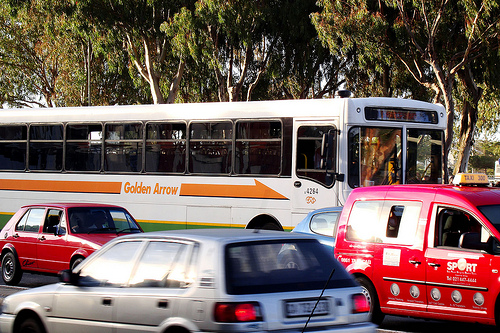
\includegraphics[width=.8\textwidth]{photos/trafficby_warrenski_flickr.jpg}
\end{minipage}

      \label{m38787*id62541}\begin{enumerate}[noitemsep, label=\textbf{\arabic*}. ] 
            \label{m38787*uid1}\item position or displacement which tells us exactly where the object is,
\label{m38787*uid2}\item speed or velocity which tells us exactly how fast the object's position is changing or more familiarly, how fast the object is moving, and
\label{m38787*uid3}\item acceleration which tells us exactly how fast the object's velocity is changing.
\end{enumerate}
      \label{m38787*id62581}You will also learn how to use position, displacement, speed, velocity and acceleration to describe the motion of simple objects. You will learn how to read and draw graphs that summarise the motion of a moving object. You will also learn about the equations that can be used to describe motion and how to apply these equations to objects moving in one dimension.\par 
    \label{m38787*cid3}
            \section{Reference point, frame of reference and position}
            \nopagebreak
\begin{minipage}{.6\textwidth}
      \label{m38787*id62597}The most important idea when studying motion, is you have to know where you are. The word \textsl{position} describes your location (where you are). However, saying that you are \textsl{here} is meaningless, and you have to specify your position \textsl{relative} to a known reference point. For example, if you are 2~m from the doorway, inside your classroom then your reference point is the doorway. This defines your position inside the classroom. Notice that you need a reference point (the doorway) and a direction (inside) to define your location.\par 
\end{minipage}
\begin{minipage}{.7\textwidth}
 \includegraphics[width=.5\textwidth]{photos/youarehereby_chokola_flickr.jpg}
\end{minipage}

      \label{m38787*uid4}
            \subsection*{Frames of reference}
            \nopagebreak
\par
\Definition{   \label{id2526298} Frame of Reference} { A frame of reference is a reference point combined with a set of directions. } 
        \label{m38787*id62648}A \textsl{frame of reference} is similar to the idea of a reference point. A frame of reference is defined as a reference point combined with a set of directions. For example, a boy is standing still inside a train as it pulls out of a station. You are standing on the platform watching the train move from left to right. To you it looks as if the boy is moving from left to right, because relative to where you are standing (the platform), he is moving. According to the boy, and his \textsl{frame of reference} (the train), he is not moving.\par 
        \label{m38787*id62666}A frame of reference must have an origin (where you are standing on the platform) and at least a positive direction. The train was moving from left to right, making to your right positive and to your left negative. If someone else was looking at the same boy, his frame of reference will be different. For example, if he was standing on the other side of the platform, the boy will be moving from right to left.\par 
        \label{m38787*eip-271}Another great example of frames of reference is a car overtaking another car on a road. Think about sitting in a taxi passing a car. If you sit in the taxi it is your origin and the direction it is moving in will be the positive direction. You will see the car slowly move further behind you (in the negative direction). The very important thing is that the driver of the car has their own reference frame in which things look different. In the driver's reference frame the taxi is moving ahead. In one case someone is falling behind, but in the other case someone is moving ahead. This is just a matter of perspective (from which reference frame you choose to view the situation).\par \label{m38787*id62675}For this chapter, we will only use frames of reference in the $x$-direction.
Frames of reference will be covered in more detail in Grade 12.\par 
    \setcounter{subfigure}{0}
\begin{figure}[H]
\begin{center}
\scalebox{1.3} % Change this value to rescale the drawing.
{
\begin{pspicture}(2.5,-1.5)(12.675,2.2879686)
%\psgrid
\psline[linewidth=0.04cm](4.26,-2.2479687)(4.26,-2.2479687)
\psline[linewidth=0.04cm](4.24,-2.1679688)(4.24,-2.1679688)
\psframe[linewidth=0.04,dimen=outer](5.06,0.47203124)(3.22,0.13203125)
\psframe[linewidth=0.04,dimen=outer](7.02,0.47203124)(5.18,0.13203125)
\psframe[linewidth=0.04,dimen=outer](9.06,0.47203124)(7.22,0.13203125)
\psline[linewidth=0.04cm](9.22,1.4920312)(9.22,0.17203125)
\psline[linewidth=0.04cm](0.0,1.6920313)(0.0,1.6920313)
\psline[linewidth=0.04cm](9.22,1.4720312)(10.02,1.4720312)
\psline[linewidth=0.04cm](10.02,1.4720312)(10.02,0.77203125)
\psline[linewidth=0.04cm](10.02,0.77203125)(11.22,0.77203125)
\psline[linewidth=0.04cm](11.22,0.77203125)(11.22,0.17203125)
\psline[linewidth=0.04cm](11.22,0.17203125)(9.22,0.17203125)
\psline[linewidth=0.04cm](10.42,1.4720312)(11.02,1.4720312)
\psline[linewidth=0.04cm](11.02,1.4720312)(10.82,0.77203125)
\psline[linewidth=0.04cm](10.42,1.4720312)(10.62,0.77203125)
\pscircle[linewidth=0.04,dimen=outer](9.82,-0.12796874){0.3}
\pscircle[linewidth=0.04,dimen=outer](10.72,-0.12796874){0.3}
\pscircle[linewidth=0.04,dimen=outer](8.52,-0.12796874){0.3}
\pscircle[linewidth=0.04,dimen=outer](7.62,-0.12796874){0.3}
\pscircle[linewidth=0.04,dimen=outer](6.52,-0.12796874){0.3}
\pscircle[linewidth=0.04,dimen=outer](5.62,-0.12796874){0.3}
\pscircle[linewidth=0.04,dimen=outer](4.62,-0.12796874){0.3}
\pscircle[linewidth=0.04,dimen=outer](3.72,-0.12796874){0.3}
\psline[linewidth=0.051999997cm](5.02,0.27203125)(5.22,0.27203125)
\psline[linewidth=0.05cm](7.02,0.27203125)(7.22,0.27203125)
\psline[linewidth=0.05cm](9.22,0.27203125)(9.02,0.27203125)
\rput{-14.036243}(-0.19131365,1.5252956){\psellipse[linewidth=0.05,dimen=outer](6.099412,1.5396783)(0.15764816,0.25)}
\psline[linewidth=0.05cm](6.04,1.3120313)(6.02,0.8720313)
\psline[linewidth=0.05cm](6.02,0.8720313)(5.82,0.47203124)
\psline[linewidth=0.05cm](5.82,0.47203124)(5.92,0.47203124)
\psline[linewidth=0.05cm](6.02,0.8720313)(6.02,0.45203125)
\psline[linewidth=0.05cm](6.02,0.47203124)(6.12,0.47203124)
\psline[linewidth=0.05cm](6.04,1.1720313)(5.92,0.97203124)
\psline[linewidth=0.05cm](5.92,0.97203124)(6.12,0.8720313)
\psdots[dotsize=0.12](6.18,1.5920312)
\psline[linewidth=0.05cm,arrowsize=0.05291667cm 2.0,arrowlength=1.4,arrowinset=0.4]{->}(9.2,1.8920312)(10.62,1.8920312)
\usefont{T1}{ptm}{m}{n}
\rput(10.585781,2.1120312){\scriptsize train moving from left to right}
\usefont{T1}{ptm}{m}{n}
\rput(6.494219,2.1120312){\scriptsize boy is standing still}
\usefont{T1}{ptm}{m}{n}
\rput(7.5909376,-0.9479687){\scriptsize From your frame of reference the boy is moving from left to right.}
\psline[linewidth=0.05cm](6.02,1.1720313)(6.06,0.8720313)
\psline[linewidth=0.05cm](6.06,0.9320313)(6.1,0.7920312)
\pscustom[linewidth=0.05]
{
\newpath
\moveto(6.08,1.4920312)
\lineto(6.11,1.4620312)
\curveto(6.125,1.4470313)(6.145,1.4270313)(6.16,1.4120313)
}
\pscustom[linewidth=0.05]
{
\newpath
\moveto(6.24,1.8120313)
\lineto(6.12,1.7820313)
\curveto(6.06,1.7670312)(5.99,1.7520312)(5.96,1.7520312)
}
\pscustom[linewidth=0.05]
{
\newpath
\moveto(6.14,1.8120313)
\lineto(6.11,1.8120313)
\curveto(6.095,1.8120313)(6.075,1.8120313)(6.07,1.8120313)
\curveto(6.065,1.8120313)(6.05,1.7920313)(6.04,1.7720313)
\curveto(6.03,1.7520312)(6.015,1.7270312)(6.0,1.7120312)
}
\end{pspicture}  
}
\end{center}
\caption{Frames of Reference}
\label{frames:boy:train}
\end{figure}   
        \label{m38787*id62702}
    \setcounter{subfigure}{0}
	\begin{figure}[H] % horizontal\label{m38787*id62705}
\begin{center}
\begin{pspicture}(0,-0.5)(5,2)
%\psgrid[gridcolor=gray]
\pcline{<->}(0.5,0.5)(4.5,0.5)
\aput{:U}{\parbox[l]{4cm}{A boy inside a train which is moving from left to right}}
\psline(2.5,0.6)(2.5,0.4)
\uput[d](2.5,0.4){Where you are standing}
\uput[d](2.5,0.0){on the platform}
\uput[d](2.5,-0.4){(reference point or origin)}
\uput[r](4.5,0.5){positive direction (towards your right)}
\uput[l](0.5,0.5){negative direction (towards your left)}
\end{pspicture}
\end{center}
 \end{figure}       
         \label{m38787*eip-509}
    \setcounter{subfigure}{0}
	\begin{figure}[H] % horizontal\label{m38787*slidesharefigure}
    \label{m38787*slidesharemedia}\label{m38787*slideshareflash}\raisebox{-5 pt}{ 
\includegraphics[width=0.5cm]{col11305.imgs/summary_www.png}} { (Presentation:  P10097 )}
      \vspace{2pt}
    \vspace{.1in}
 \end{figure}       \par 
      \label{m38787*uid6}
            \subsection*{Position}
            \nopagebreak
\Definition{ Position } { Position is a measurement of a location, with reference to an origin.  } 
        \label{m38787*id62737}A position is a measurement of a location, with reference to an origin. Positions can therefore be negative or positive. The symbol $x$ is used to indicate position. $x$ has units of length for example cm, m or km.
Figure~20.4 shows the position of a school. Depending on what reference point we choose, we can say that the school is $300\phantom{\rule{2pt}{0ex}}\mathsf{m}$ from Joan's house (with Joan's house as the reference point or origin) or  $500\phantom{\rule{2pt}{0ex}}\mathsf{m}$ from Joel's house (with Joel's house as the reference point or origin).\par 
    \setcounter{subfigure}{0}
\begin{figure}[H]
\begin{center}
\scalebox{1} % Change this value to rescale the drawing.
{
\begin{pspicture}(0,-1.421875)(14.005,1.386875)
\psframe[linewidth=0.05,dimen=outer](1.82,0.601875)(0.22,-0.298125)
\pstriangle[linewidth=0.05,dimen=outer](1.03,0.541875)(2.06,0.82)
\pstriangle[linewidth=0.05,dimen=outer](13.03,0.561875)(2.06,0.82)
\psline[linewidth=0.05cm,tbarsize=0.07055555cm 5.0]{|-|}(1.06,-0.918125)(13.1,-0.938125)
\psline[linewidth=0.05cm](3.08,-0.798125)(3.08,-1.038125)
\psline[linewidth=0.05cm](5.06,-0.798125)(5.06,-1.038125)
\psline[linewidth=0.05cm](7.06,-0.818125)(7.06,-1.038125)
\psline[linewidth=0.05cm](9.06,-0.798125)(9.06,-1.038125)
\psline[linewidth=0.05cm](11.06,-0.778125)(11.06,-1.018125)
\usefont{T1}{ptm}{m}{n}
\rput(2.085,-1.283125){\footnotesize 100 m}
\psframe[linewidth=0.05,dimen=outer](13.86,0.621875)(12.26,-0.278125)
\psframe[linewidth=0.05,dimen=outer](3.52,0.581875)(2.64,-0.298125)
\psframe[linewidth=0.05,dimen=outer](5.5,0.581875)(4.62,-0.298125)
\psframe[linewidth=0.05,dimen=outer](7.5,0.581875)(6.62,-0.298125)
\psframe[linewidth=0.05,dimen=outer](9.52,0.581875)(8.64,-0.298125)
\psframe[linewidth=0.05,dimen=outer](11.52,0.581875)(10.64,-0.298125)
\pstriangle[linewidth=0.05,dimen=outer](3.08,0.521875)(1.36,0.54)
\pstriangle[linewidth=0.05,dimen=outer](7.06,0.521875)(1.36,0.54)
\pstriangle[linewidth=0.05,dimen=outer](5.04,0.521875)(1.36,0.54)
\pstriangle[linewidth=0.05,dimen=outer](9.06,0.521875)(1.36,0.54)
\pstriangle[linewidth=0.05,dimen=outer](11.08,0.521875)(1.36,0.54)
\usefont{T1}{ptm}{m}{n}
\rput(4.105,-1.263125){\footnotesize 100 m}
\usefont{T1}{ptm}{m}{n}
\rput(6.105,-1.283125){\footnotesize 100 m}
\usefont{T1}{ptm}{m}{n}
\rput(8.125,-1.263125){\footnotesize 100 m}
\usefont{T1}{ptm}{m}{n}
\rput(10.125,-1.263125){\footnotesize 100 m}
\usefont{T1}{ptm}{m}{n}
\rput(12.125,-1.283125){\footnotesize 100 m}
\usefont{T1}{ptm}{m}{n}
\rput(13.068594,0.161875){\small Shop}
\usefont{T1}{ptm}{m}{n}
\rput(1.065,0.171875){School}
\usefont{T1}{ptm}{m}{n}
\rput(3.0773437,0.171875){Jack}
\usefont{T1}{ptm}{m}{n}
\rput(5.0554686,0.171875){John}
\usefont{T1}{ptm}{m}{n}
\rput(7.065469,0.171875){Joan}
\usefont{T1}{ptm}{m}{n}
\rput(9.0725,0.171875){Jill}
\usefont{T1}{ptm}{m}{n}
\rput(11.065469,0.171875){Joel}
\end{pspicture} 
}
\end{center}
\label{position:reference3}
\caption{Illustration of position}
\end{figure}      
        \label{m38787*id62778}The shop is also $300\phantom{\rule{2pt}{0ex}}m$ from Joan's house, but in the opposite direction as the school. When we choose a reference point, we have a positive direction and a negative direction. If we choose the direction towards the school as positive, then the direction towards the shop is negative. A negative direction is always opposite to the direction chosen as positive.\par 
    \setcounter{subfigure}{0}
\begin{figure}[H]
\begin{center}
\scalebox{1} % Change this value to rescale the drawing.
{
\begin{pspicture}(0,-1.1871876)(9.225,1.1871876)
\psline[linewidth=0.05cm,arrowsize=0.05291667cm 2.0,arrowlength=1.4,arrowinset=0.4]{<->}(0.0,-0.6428125)(8.0,-0.6428125)
\psline[linewidth=0.05cm](1.02,-0.5028125)(1.02,-0.7828125)
\psline[linewidth=0.05cm](2.02,-0.5028125)(2.02,-0.7828125)
\psline[linewidth=0.05cm](3.0,-0.5028125)(3.0,-0.7828125)
\psline[linewidth=0.05cm](4.02,-0.5028125)(4.02,-0.7828125)
\psline[linewidth=0.05cm](5.02,-0.5028125)(5.02,-0.7828125)
\psline[linewidth=0.05cm](6.02,-0.5028125)(6.02,-0.7828125)
\psline[linewidth=0.05cm](7.02,-0.5028125)(7.02,-0.7828125)
\usefont{T1}{ptm}{m}{n}
\rput(0.97625,-1.0328125){+300}
\usefont{T1}{ptm}{m}{n}
\rput(1.97625,-1.0328125){+200}
\usefont{T1}{ptm}{m}{n}
\rput(2.97625,-1.0328125){+100}
\usefont{T1}{ptm}{m}{n}
\rput(3.9970312,-1.0128125){0}
\usefont{T1}{ptm}{m}{n}
\rput(5.0025,-1.0128125){-100}
\usefont{T1}{ptm}{m}{n}
\rput(6.0196877,-1.0128125){-200}
\usefont{T1}{ptm}{m}{n}
\rput(7.01625,-1.0128125){-300}
\psline[linewidth=0.05cm,arrowsize=0.05291667cm 2.0,arrowlength=1.4,arrowinset=0.4]{->}(1.0,0.2971875)(1.0,-0.4428125)
\psline[linewidth=0.05cm,arrowsize=0.05291667cm 2.0,arrowlength=1.4,arrowinset=0.4]{->}(4.02,0.3171875)(4.02,-0.4628125)
\psline[linewidth=0.05cm,arrowsize=0.05291667cm 2.0,arrowlength=1.4,arrowinset=0.4]{->}(7.02,0.2971875)(7.02,-0.4828125)
\usefont{T1}{ptm}{m}{n}
\rput(0.965,0.6871875){School}
\usefont{T1}{ptm}{m}{n}
\rput(4.101094,1.0071875){Joan's house}
\usefont{T1}{ptm}{m}{n}
\rput(4.1451564,0.6071875){(reference point)}
\usefont{T1}{ptm}{m}{n}
\rput(7.012656,0.6871875){Shop}
\usefont{T1}{ptm}{m}{n}
\rput(8.612968,-0.5928125){$x$ (m)}
\end{pspicture}  }
\caption{The origin is at Joan's house and the position of the school is +300~m. Positions towards the left are defined as positive and positions towards the right are defined as negative.}
\label{pr:position:reference2}
\end{center}
\end{figure}      
\label{m38787*secfhsst!!!underscore!!!id127}
\begin{groupdiscussion}{Reference Points }
            \nopagebreak
        \label{m38787*id62809}Divide into groups of 5 for this activity.
On a straight line, choose a reference point. Since position can have both positive and negative values, discuss the advantages and disadvantages of choosing\par 
        \label{m38787*id62816}\begin{enumerate}[noitemsep, label=\textbf{\arabic*}. ] 
            \label{m38787*uid9}\item either end of the line,
\label{m38787*uid10}\item the middle of the line.
\end{enumerate}
\end{groupdiscussion}
        \label{m38787*id62843}This reference point can also be called ``the origin". \par 
\label{m38787*secfhsst!!!underscore!!!id138}
\begin{exercises}{Position }
            \nopagebreak
        \label{m38787*id62859}\begin{enumerate}[noitemsep, label=\textbf{\arabic*}. ] 
            \label{m38787*uid11}\item Write down the positions for objects at A, B, D and E. Do not forget the units.
    \setcounter{subfigure}{0}
	\begin{figure}[H] % horizontal\label{m38787*id62877}
\begin{center}
\begin{pspicture*}(-6,-1)(6.1,1)
\psset{dotsize=7pt}
%\psgrid[gridcolor=lightgray]
\multirput(0,0)(0,0){1}{
\multido{\n=-4+1}{9}
{\psline{<->}(-5,0)(5,0)
\rput(\n,0){\psline(0,-0.1)(0,0.1)}
\uput[d](\n,-0.1){\n}}
\uput[r](5,0){$x$ (m)}}
\uput[u](0,0.5){reference point}
\uput[u](-3,0.2){A}
\uput[u](-1,0.2){B}
\uput[u](1,0.2){D}
\uput[u](3,0.2){E}
\psline{->}(0,0.6)(0,0.2)
\end{pspicture*}
\end{center}
 \end{figure}
\label{m38787*uid12}\item Write down the positions for objects at F, G, H and J. Do not forget the units.
    \setcounter{subfigure}{0}
	\begin{figure}[H] % horizontal\label{m38787*id62899}
\begin{center}
\begin{pspicture*}(-6,-1)(6.1,1)
\psset{dotsize=7pt}
%\psgrid[gridcolor=lightgray]
\multirput(0,0)(0,0){1}{
\multido{\n=-4+1}{9}
{\psline{<->}(-5,0)(5,0)
\rput(\n,0){\psline(0,-0.1)(0,0.1)}
\uput[d](-\n,-0.1){\n}}
\uput[r](5,0){$x$ (m)}}
\uput[u](0,0.5){reference point}
\uput[u](-3,0.2){F}
\uput[u](-1,0.2){G}
\uput[u](1,0.2){H}
\uput[u](3,0.2){J}
\psline{->}(0,0.6)(0,0.2)
\end{pspicture*}
\end{center}
 \end{figure}
\label{m38787*uid13}\item There are 5 houses on Newton Street, A, B, C, D and E. For all cases, assume that positions to the right are positive.
    \setcounter{subfigure}{0}
	\begin{figure}[H] % horizontal\label{m38787*id62920}
\begin{center}
\begin{pspicture*}(-4.2,-0.2)(5.2,2.8)
\def\house{\psframe(0,0)(1,1)\pspolygon(0,1)(0.5,2)(1,1)}
\def\distance{\psline(0.5,2.2)(0.5,2.4)\psline(2.5,2.2)(2.5,2.4)\psline{<->}(0.5,2.3)(2.5,2.3)\uput[u](1.5,2.3){20 m}}
\psset{dotsize=7pt}
%\psgrid[gridcolor=lightgray]
\multirput(-4,0)(2,0){5}{\house}
\multirput(-4,0)(2,0){4}{\distance}
\rput(-3.5,0.5){\Large{\textsf{A}}}
\rput(-1.5,0.5){\Large{\textsf{B}}}
\rput(0.5,0.5){\Large{\textsf{C}}}
\rput(2.5,0.5){\Large{\textsf{D}}}
\rput(4.5,0.5){\Large{\textsf{E}}}
\end{pspicture*}
\end{center}
 \end{figure}       \label{m38787*id62926}\begin{enumerate}[noitemsep, label=\textbf{\alph*}. ] 
            \label{m38787*uid14}\item Draw a frame of reference with house A as the origin and write down the positions of houses B, C, D and E.
\label{m38787*uid15}\item You live in house C. What is your position relative to house E?
\label{m38787*uid16}\item What are the positions of houses A, B and D, if house B is taken as the reference point?
\end{enumerate}
                \end{enumerate}
  \label{m38787**end}
\par \raisebox{-5 pt}{
\includegraphics[width=0.5cm]{col11305.imgs/summary_www.png}} Find the answers with the shortcodes:
 \par \begin{tabular}[h]{cccccc}
 (1.) laG  &  (2.) la7  &  (3.) laA  & \end{tabular}
\end{exercises}
         \subsection*{Displacement and distance}
    \nopagebreak
            \label{m38788} $ \hspace{-5pt}\begin{array}{cccccccccccc}   \end{array} $ \hspace{2 pt}\raisebox{-5 pt}{
\includegraphics[width=0.5cm]{col11305.imgs/summary_www.png}} {(section shortcode: P10098 )} \par 
\Definition{ Displacement } {Displacement is the change in an object's position.  } 
      \end{tabular*}
      \end{definition}
      \label{m38788*id63003}The displacement of an object is defined as its change in position (final position minus initial position). Displacement has a magnitude and direction and is therefore a vector. For example, if the initial position of a car is ${x}_{i}$ and it moves to a final position of ${x}_{f}$, then the displacement is:\par 
      \label{m38788*id63035}\nopagebreak\noindent{}
        
    \begin{equation}
    {x}_{f}-{x}_{i}
      \end{equation}
      \label{m38788*id63061}However, subtracting an initial quantity from a final quantity happens often in Physics, so we use the shortcut $\Delta $ to mean \textsl{final - initial}. Therefore, displacement can be written:\par 
      \label{m38788*id63080}\nopagebreak\noindent{}
        
    \begin{equation}
    \Delta x={x}_{f}-{x}_{i}
      \end{equation}
\label{m38788*notfhsst!!!underscore!!!id194}
\Tip{The symbol $\Delta $ is read out as \textsl{delta}. $\Delta $ is a letter of the Greek alphabet and is used in Mathematics and Science to indicate a change in a certain quantity, or a final value minus an initial value. For example, $\Delta x$ means change in $x$ while $\Delta t$ means change in $t$.}
\Tip{The words \textsl{initial} and \textsl{final} will be used very often in Physics. \textsl{Initial} will always refer to something that happened earlier in time and \textsl{final} will always refer to something that happened later in time. It will often happen that the final value is smaller than the initial value, such that the difference is negative. This is ok!}
    \setcounter{subfigure}{0}
\begin{figure}[H]
\begin{center}
\begin{pspicture}(0.2,0.2)(5,5)
%\psgrid[gridcolor=lightgray]
\psdots(0.5,1)\psdots(4.5,4.5)
\pscurve[linestyle=dashed](0.5,1)(1,2)(2,4)(2.5,2)(4,4)(4.5,4.5)
\rput(0.5,0.8){Start}
\rput(0.5,0.4){(School)}
\rput(4.5,5.1){Finish}
\rput(4.5,4.7){(Shop)}
\psline[linewidth=0.05, linestyle=dotted, arrowscale=2]{->}(0.5,1)(4.4,1)
\psline[linewidth=0.05, linestyle=dotted,arrowscale=2]{->}(4.4,1)(4.4,4.4)
\pcline[arrowscale=2]{->}(0.5,1)(4.5,4.5)
\lput*{:U}{Displacement}
\end{pspicture}
\end{center}
\caption{Illustration of displacement}
\label{vectors:displ}
\end{figure}       
\label{m38788*id63218}Displacement does not depend on the path travelled, but only on the initial and final positions (Figure~\ref{vectors:displ}). We use the word \textsl{distance} to describe how far an object travels along a particular path. Distance is the actual distance that was covered. Distance (symbol $D$) does not have a direction, so it is a scalar. Displacement is the shortest distance from the starting point to the endpoint -- from the school to the shop in the figure. Displacement has direction and is therefore a vector.\par 
\label{m38788*id62109} shows the five houses we discussed earlier. Jack walks to school, but instead of walking straight to school, he decided to walk to his friend Joel's house first to fetch him so that they can walk to school together. Jack covers a distance of $400\phantom{\rule{2pt}{0ex}}\mathsf{m}$ to Joel's house and another $500\phantom{\rule{2pt}{0ex}}\mathsf{m}$ to school. He covers a distance of $900\phantom{\rule{2pt}{0ex}}\mathsf{m}$. His displacement, however, is only $100\phantom{\rule{2pt}{0ex}}\mathsf{m}$ towards the school. This is because displacement only looks at the starting position (his house) and the end position (the school). It does not depend on the path he travelled.\par 
\label{m38788*id62121}To calculate his distance and displacement, we need to choose a reference point and a direction. Let's choose Jack's house as the reference point, and towards Joel's house as the positive direction (which means that towards the school is negative). We would do the calculations as follows:\\
\begin{minipage}{0.5\textwidth}
\begin{eqnarray*}
\mathsf{Distance (d)} &=& \mathsf{path~travelled}\\
&=&400\ \mathsf{m} + 500\ \mathsf{m}\\
&=&900\ \mathsf{m}\\
\end{eqnarray*}
\end{minipage}
\begin{minipage}{0.5\textwidth}
\begin{eqnarray*}
\mathsf{Displacement} (\Delta x) &=& x_f~ - ~ x_i\\
&=&-100\ \mathsf{m} + 0\ \mathsf{m}\\
&=&-100\ \mathsf{m}\\
%&=&100\ \mathsf{m} towards the school
\end{eqnarray*}
\end{minipage}
      \label{m38788*eip-883}
\Tip{We will use $\mathsf{D}$ in this book, but you may see $\mathsf{d}$ used in other books.}
      \label{m38788*id63667}Joel walks to school with Jack and after school walks back home. What is Joel's displacement and what distance did he cover?
For this calculation we use Joel's house as the reference point. Let's take towards the school as the positive direction.\\
\begin{minipage}{0.5\textwidth}
\begin{eqnarray*}
\mathsf{Distance (d)} &=& \mathsf{path~travelled}\\
&=&500\ \mathsf{m} + 500\ \mathsf{m}\\
&=&1000\ \mathsf{m}
\end{eqnarray*}
\end{minipage}
\begin{minipage}{0.5\textwidth}
\begin{eqnarray*}
\mathsf{Displacement} (\Delta x) &=& x_f~ - ~ x_i\\
&=&0\ \mathsf{m} + 0\ \mathsf{m}\\
&=&0\ \mathsf{m}
\end{eqnarray*}
\end{minipage} 
      \label{m38788*id63886}It is possible to have a displacement of $0\phantom{\rule{2pt}{0ex}}\mathsf{m}$ and a distance that is not $0\phantom{\rule{2pt}{0ex}}\mathsf{m}$. This happens when an object completes a round trip back to its original position, like an athlete running around a track.\par 
      \label{m38788*uid18}
            \subsubsection*{Interpreting Direction}
            \nopagebreak
        \label{m38788*id63901}Very often in calculations you will get a negative answer. For example, Jack's displacement in the example above, is calculated as $-100\phantom{\rule{2pt}{0ex}}\mathsf{m}$. The minus sign in front of the answer means that his displacement is $100\phantom{\rule{2pt}{0ex}}\mathsf{m}$ in the opposite direction (opposite to the direction chosen as positive in the beginning of the question). When we start a calculation we choose a frame of reference and a positive direction. In the first example above, the reference point is Jack's house and the positive direction is towards Joel's house. Therefore Jack's displacement is $100\phantom{\rule{2pt}{0ex}}\mathsf{m}$ towards the school. Notice that distance has no direction, but displacement has.\par 
      \label{m38788*uid19}
            \subsubsection*{Differences between Distance and Displacement}
            \nopagebreak
        \label{m38788*id63938}The differences between distance and displacement can be summarised as:\par 
\begin{center}
\begin{tabular}{|l|l|}\hline
\textbf{ Distance } & \textbf{ Displacement } \\\hline
1. depends on the path & 1. independent of path taken \\\hline
2. always positive & 2. can be positive or negative \\\hline
3. is a scalar & 3. is a vector\\\hline
\end{tabular}
\end{center}
    \par
\label{m38788*secfhsst!!!underscore!!!id498}
\begin{exercises}{Frames of reference, displacement and distance}
            \nopagebreak
        \label{m38788*id64042}\begin{enumerate}[noitemsep, label=\textbf{\arabic*}. ] 
            \label{m38788*uid20}\item Use  to answer the following questions.
\label{m38788*id64060}\begin{enumerate}[noitemsep, label=\textbf{\alph*}. ] 
            \label{m38788*uid21}\item Jill walks to Joan's house and then to school, what is her distance and displacement?
\label{m38788*uid22}\item John walks to Joan's house and then to school, what is his distance and displacement?
\label{m38788*uid23}\item Jack walks to the shop and then to school, what is his distance and displacement?
\label{m38788*uid24}\item What reference point did you use for each of the above questions?
\end{enumerate}
                \label{m38788*uid25}\item You stand at the front door of your house (displacement, $\Delta x=0\phantom{\rule{2pt}{0ex}}\mathsf{m}$). The street is $10\phantom{\rule{2pt}{0ex}}\mathsf{m}$ away from the front door. You walk to the street and back again.
\label{m38788*id64141}\begin{enumerate}[noitemsep, label=\textbf{\alph*}. ] 
            \label{m38788*uid26}\item What is the distance you have walked?
\label{m38788*uid27}\item What is your final displacement?
\label{m38788*uid28}\item Is displacement a vector or a scalar? Give a reason for your answer.
\end{enumerate}
                \end{enumerate}
  \label{m38788**end}
\par \raisebox{-5 pt}{
\includegraphics[width=0.5cm]{col11305.imgs/summary_www.png}} Find the answers with the shortcodes:
 \par \begin{tabular}[h]{cccccc}
 (1.) lao  &  (2.) las  & \end{tabular}
\end{exercises}
         \section{Average speed, average velocity and acceleration} 
    \nopagebreak
            \label{m38791} $ \hspace{-5pt}\begin{array}{cccccccccccc}   
\includegraphics[width=0.75cm]{col11305.imgs/summary_fullmarks.png} &   \end{array} $ \hspace{2 pt}\raisebox{-5 pt}{} {(section shortcode: P10099 )} \par 
    \label{m38791*cid5}
            \subsection*{Speed, average velocity and instantaneous velocity}
            \nopagebreak
\Definition{ Velocity } { Velocity is the rate of change of displacement. } 
\Definition{ Instantaneous velocity } { Instantaneous velocity is the velocity of a body at a specific instant in time. } 
\Definition{ Average velocity } {Average velocity is the total displacement of a body over a time interval. } 
      \label{m38791*id64258}Velocity is the rate of change of position. It tells us how much an object's position changes in time. This is the same as the displacement divided by the time taken. Since displacement is a vector and time taken is a scalar, velocity is also a vector. We use the symbol $v$ for velocity. If we have a displacement of $\Delta x$ and a time taken of $\Delta t$, $v$ is then defined as:\par 
      \label{m38791*id64307}\nopagebreak\noindent{}
\begin{eqnarray*}
\mathsf{velocity\ (in\ m} \cdot \mathsf{s}^{-1}) &=& \frac{\mathsf{change\ in\ displacement\ (in\ m)}}{\mathsf{change\ in\ time\ (in\ s)}}\\
v &=& \frac{\Delta x}{\Delta t}
\end{eqnarray*}\label{eq:pr:velocity}
      \label{m38791*id64460}Velocity can be positive or negative. Positive values of velocity mean that the object is moving away from the reference point or origin and negative values mean that the object is moving towards the reference point or origin.\par 
\label{m38791*notfhsst!!!underscore!!!id615}
\Tip{An instant in time is different from the time taken or the time interval. It is therefore useful to use the symbol $t$ for an instant in time (for example during the 4$^\text{th}$ second) and the symbol $\Delta t$ for the time taken (for example during the first 5 seconds of the motion).}
      \label{m38791*id64500}Average velocity (symbol $v$) is the displacement for the whole motion divided by the time taken for the whole motion. Instantaneous velocity is the velocity at a specific instant in time.\par 
      \label{m38791*eip-536}This is terminology that occurs quite often and it is important to always remember that instantaneous and average quantities are not always the same. In fact, they can be very different. The magnitude of the instantaneous velocity is the same as the slope of the line which is a tangent to the displacement curve at the time of measurement. The magnitude of the average velocity is the same as the slope of the line between the start and end points of the interval. \par \label{m38791*eip-668}If you want to think about why the tangent at a particular time gives us the velocity remember that the velocity is the slope of the displacement curve. Now, a simple why to start thinking about it is to image you could zoom (magnify) the displacement curve at the point. The more you zoom in the more it will look like a straight line at the point and that straight line will be very similar to the tangent line at the point. This isn't a mathematical proof but you will learn one later on in mathematics about limits and slopes. \par \label{m38791*id64514}(Average) Speed (symbol $s$) is the distance travelled ($D$) divided by the time taken ($\Delta t$) for the journey. Distance and time are scalars and therefore speed will also be a scalar. Speed is calculated as follows:\par 
      \label{m38791*id64549}\nopagebreak\noindent{}
        
    \begin{equation}
    \mathsf{speed}\phantom{\rule{4pt}{0ex}}\left(\mathsf{in}\phantom{\rule{4pt}{0ex}}\mathsf{m}\ensuremath{\cdot}{\mathsf{s}}^{-1}\right)=\frac{\mathsf{distance}\phantom{\rule{4pt}{0ex}}\left(\mathsf{in}\phantom{\rule{4pt}{0ex}}\mathsf{m}\right)}{\mathsf{time}\phantom{\rule{4pt}{0ex}}\left(\mathsf{in}\phantom{\rule{4pt}{0ex}}\mathsf{s}\right)}
      \end{equation}
      \label{m38791*id64639}\nopagebreak\noindent{}
    \begin{equation}
    s=\frac{D}{\Delta t}
      \end{equation}
      \label{m38791*id64664}Instantaneous speed is the magnitude of instantaneous velocity. It has the same value, but no direction.\par 
\begin{wex}{Average speed and average velocity}
{James walks 2~km away from home in 30 minutes. He then turns around and walks back home along the same path, also in 30 minutes. Calculate James' average speed and average velocity.\\
\begin{center}
\begin{pspicture}(0,0)(3,0.5)
%\psgrid
\psline[linewidth=1pt]{->}(0,0)(2,0)
\psline[linewidth=1pt]{->}(2,0.5)(0,0.5)
\psarc[linewidth=1pt]{->}(2.1,0.25){0.25}{-90}{90}
\uput[d](1,1){2 km}
\end{pspicture}
\end{center}}
{\westep{Identify what information is given and what is asked for}
The question explicitly gives
\begin{itemize}
\item the distance and time out (2 km in 30 minutes)
\item the distance and time back (2 km in 30 minutes)
\end{itemize}

\westep{Check that all units are SI units.}
The information is not in SI units and must therefore be converted.\\
To convert km to m, we know that:
\begin{eqnarray*}
1\ \mathsf{km} &=&1\ 000\ \mathsf{m}\\
\therefore\quad 2\ \mathsf{km} &=&2\ 000\ \mathsf{m} \quad \mbox{(multiply both sides by 2, because we want to convert 2 km to m.)}
\end{eqnarray*}
Similarly, to convert 30 minutes to seconds,
\begin{eqnarray*}
1\ \mathsf{min} &=&60 \mathsf{s}\\
\therefore\quad 30\ \mathsf{min} &=&1\ 800\ \mathsf{s} \quad \mbox{(multiply both sides by 30)}
\end{eqnarray*}

\westep{Determine James' displacement and distance.}
James started at home and returned home, so his displacement is 0 m.\\
$\Delta x = 0\ \mathsf{m}$\\
James walked a total distance of 4 000~m (2 000~m out and 2 000~m back).\\
$d = 4\ 000\;\mathsf{m}$

\westep{Determine his total time.}
James took 1~800~s to walk out and 1~800~s to walk back.\\
$\Delta t = 3\ 600\;\mathsf{s}$

\westep{Determine his average speed}
\begin{eqnarray*}
s&=&\frac{d}{\Delta t}\\
&=&\frac{4\ 000\ \mathsf{m}}{3\ 600\ \mathsf{s}}\\
&=&1,11\ \ems
\end{eqnarray*}

\westep{Determine his average velocity}
\begin{eqnarray*}
{v}&=&\frac{\Delta x}{\Delta t}\\
&=&\frac{0\ \mathsf{m}}{3\ 600\ \mathsf{s}}\\
&=& 0\ \ems
\end{eqnarray*}}
\end{wex}
    \noindent
      \label{m38791*uid37}
            \subsubsection*{Differences between Speed and Velocity}
            \nopagebreak
        \label{m38791*id66482}The differences between speed and velocity can be summarised as:\par 
\begin{center}
\begin{tabular}{|p{5cm}|p{5cm}|}\hline
\textbf{Speed} & \textbf{Velocity} \\\hline
1. depends on the path taken & 1. independent of path taken \\\hline
2. always positive & 2. can be positive or negative \\\hline
3. is a scalar & 3. is a vector \\\hline
4. no dependence on direction and so is only positive & 4. direction can be guessed from the sign (i.e. positive or negative) \\\hline
\end{tabular}
\end{center}
    \par
        \label{m38791*id66611}Additionally, an object that makes a round trip, i.e. travels away from its starting point and then returns to the same point has zero velocity but travels a non-zero speed.\par 
\label{m38791*secfhsst!!!underscore!!!id1252}
\begin{exercises}{Displacement and related quantities }
            \nopagebreak
        \label{m38791*id66624}\begin{enumerate}[noitemsep, label=\textbf{\arabic*}. ] 
            \label{m38791*uid38}\item Theresa has to walk to the shop to buy some milk. After walking $100\phantom{\rule{2pt}{0ex}}\mathsf{m}$, she realises that she does not have enough money, and goes back home. If it took her two minutes to leave and come back, calculate the following:
\label{m38791*id66641}\begin{enumerate}[noitemsep, label=\textbf{\alph*}. ] 
            \label{m38791*uid39}\item How long was she out of the house (the time interval $\Delta t$ in seconds)?
\label{m38791*uid40}\item How far did she walk (distance (D))?
\label{m38791*uid41}\item What was her displacement ($\Delta x$)?
\label{m38791*uid42}\item What was her average velocity (in m$\ensuremath{\cdot}$s${}^{-1}$)?
\label{m38791*uid43}\item What was her average speed (in m$\ensuremath{\cdot}$s${}^{-1}$)?
\end{enumerate}
    \setcounter{subfigure}{0}
	\begin{figure}[H] % horizontal\label{m38791*id66785}
\begin{center}
\scalebox{0.5} % Change this value to rescale the drawing.
{%girl walking
\begin{pspicture}(0,-3.7525)(6.5721874,3.7325)
%\definecolor{color816g}{rgb}{0.4,0.4,0.4}
\psellipse[linewidth=0.04,dimen=outer](5.1325,2.8925)(0.55,0.8)
\psline[linewidth=0.04cm](5.1825,2.0925)(5.4825,0.5925)
\psline[linewidth=0.04cm](5.2825,1.6925)(5.6825,0.7925)
\psline[linewidth=0.04cm](5.2825,1.5925)(5.2825,0.5925)
\psline[linewidth=0.04cm](5.2825,0.5925)(4.7825,0.4925)
\psline[linewidth=0.04cm](5.4825,0.5925)(5.1825,-0.8075)
\psline[linewidth=0.04cm](5.1825,-0.8075)(5.3825,-2.1075)
\psline[linewidth=0.04cm](5.3825,-2.1075)(5.0825,-2.1075)
\psline[linewidth=0.04cm](5.4825,0.5925)(5.4825,-0.7075)
\psline[linewidth=0.04cm](5.4825,-0.7075)(5.6825,-1.9075)
\psline[linewidth=0.04cm](5.6825,-1.9075)(5.4825,-2.1075)
%\rput{7.3992243}(0.12179666,-0.693829){\pstriangle[linewidth=0.04,dimen=outer,fillstyle=gradient,gradlines=2000,gradbegin=color816g,gradend=color816g,gradmidpoint=1.0](5.4260836,-0.5557346)(0.76654965,2.301279)}
\rput{7.3992243}(0.12179666,-0.693829){\pstriangle[linewidth=0.04,dimen=outer,fillstyle=gradient,gradlines=2000](5.4260836,-0.5557346)(0.76654965,2.301279)}
\psline[linewidth=0.04cm](5.6825,0.7925)(5.0825,0.1925)
\psdots[dotsize=0.12](4.8425,3.0525)
\pscustom[linewidth=0.04]
{
\newpath
\moveto(4.7025,2.4125)
}
\pscustom[linewidth=0.04]
{
\newpath
\moveto(5.0425,2.6325)
\lineto(4.9825,2.5825)
\curveto(4.9525,2.5575)(4.8875,2.5125)(4.8525,2.4925)
\curveto(4.8175,2.4725)(4.7625,2.4525)(4.7025,2.4525)
}
\pscustom[linewidth=0.04]
{
\newpath
\moveto(5.3225,3.5325)
\lineto(5.3625,3.3225)
\curveto(5.3825,3.2175)(5.4325,2.9625)(5.4625,2.8125)
\curveto(5.4925,2.6625)(5.5575,2.4275)(5.5925,2.3425)
\curveto(5.6275,2.2575)(5.7075,2.1725)(5.7525,2.1725)
\curveto(5.7975,2.1725)(5.8825,2.1975)(5.9225,2.2225)
\curveto(5.9625,2.2475)(6.0425,2.3125)(6.0825,2.3525)
}
\pscustom[linewidth=0.04]
{
\newpath
\moveto(6.0825,2.3525)
\lineto(5.9825,2.3825)
\curveto(5.9325,2.3975)(5.8625,2.4375)(5.8425,2.4625)
\curveto(5.8225,2.4875)(5.8025,2.5725)(5.8025,2.6325)
\curveto(5.8025,2.6925)(5.7725,2.8325)(5.7425,2.9125)
\curveto(5.7125,2.9925)(5.6625,3.1175)(5.6425,3.1625)
\curveto(5.6225,3.2075)(5.6025,3.2925)(5.6025,3.3325)
\curveto(5.6025,3.3725)(5.5625,3.4625)(5.5225,3.5125)
\curveto(5.4825,3.5625)(5.4125,3.6375)(5.3825,3.6625)
\curveto(5.3525,3.6875)(5.2975,3.7125)(5.2725,3.7125)
\curveto(5.2475,3.7125)(5.1775,3.7125)(5.1325,3.7125)
\curveto(5.0875,3.7125)(5.0225,3.6925)(5.0025,3.6725)
\curveto(4.9825,3.6525)(4.9325,3.6275)(4.9025,3.6225)
\curveto(4.8725,3.6175)(4.7975,3.5675)(4.7525,3.5225)
\curveto(4.7075,3.4775)(4.6525,3.3875)(4.6425,3.3425)
\curveto(4.6325,3.2975)(4.6175,3.2475)(4.6025,3.2325)
}
\pscustom[linewidth=0.04]
{
\newpath
\moveto(4.6025,3.2525)
\lineto(4.6725,3.2725)
\curveto(4.7075,3.2825)(4.7575,3.3175)(4.7725,3.3425)
\curveto(4.7875,3.3675)(4.8575,3.4325)(4.9125,3.4725)
\curveto(4.9675,3.5125)(5.0575,3.5575)(5.0925,3.5625)
\curveto(5.1275,3.5675)(5.1925,3.5725)(5.2225,3.5725)
\curveto(5.2525,3.5725)(5.2925,3.5575)(5.3025,3.5425)
\curveto(5.3125,3.5275)(5.3275,3.5075)(5.3425,3.4925)
}

\pscustom[linewidth=0.04]
{
\newpath
\moveto(4.6425,3.3725)
\lineto(4.6825,3.3925)
\curveto(4.7025,3.4025)(4.7275,3.4275)(4.7325,3.4425)
\curveto(4.7375,3.4575)(4.7425,3.4575)(4.7425,3.4425)
\curveto(4.7425,3.4275)(4.7725,3.4325)(4.8025,3.4525)
\curveto(4.8325,3.4725)(4.8825,3.5125)(4.9025,3.5325)
\curveto(4.9225,3.5525)(4.9325,3.5875)(4.9225,3.6025)
\curveto(4.9125,3.6175)(4.9625,3.6325)(5.0225,3.6325)
\curveto(5.0825,3.6325)(5.1175,3.6325)(5.0925,3.6325)
\curveto(5.0675,3.6325)(5.0975,3.6325)(5.1525,3.6325)
\curveto(5.2075,3.6325)(5.3025,3.6075)(5.3425,3.5825)
\curveto(5.3825,3.5575)(5.4325,3.5175)(5.4425,3.5025)
\curveto(5.4525,3.4875)(5.4375,3.4675)(5.4125,3.4625)
\curveto(5.3875,3.4575)(5.4225,3.3725)(5.4825,3.2925)
\curveto(5.5425,3.2125)(5.6275,3.0825)(5.6525,3.0325)
\curveto(5.6775,2.9825)(5.7025,2.8825)(5.7025,2.8325)
\curveto(5.7025,2.7825)(5.7225,2.6575)(5.7425,2.5825)
\curveto(5.7625,2.5075)(5.7875,2.3975)(5.7925,2.3625)
\curveto(5.7975,2.3275)(5.8525,2.3025)(5.9025,2.3125)
\curveto(5.9525,2.3225)(5.9675,2.3275)(5.9325,2.3225)
\curveto(5.8975,2.3175)(5.8125,2.3175)(5.7625,2.3225)
\curveto(5.7125,2.3275)(5.6525,2.4325)(5.6425,2.5325)
\curveto(5.6325,2.6325)(5.5625,2.9275)(5.5025,3.1225)
\curveto(5.4425,3.3175)(5.3775,3.4925)(5.3725,3.4725)
\curveto(5.3675,3.4525)(5.3775,3.2925)(5.3925,3.1525)
\curveto(5.4075,3.0125)(5.4575,2.8225)(5.4925,2.7725)
\curveto(5.5275,2.7225)(5.5675,2.6275)(5.5725,2.5825)
\curveto(5.5775,2.5375)(5.5975,2.4475)(5.6125,2.4025)
\curveto(5.6275,2.3575)(5.6725,2.2975)(5.7025,2.2825)
\curveto(5.7325,2.2675)(5.7975,2.2525)(5.8325,2.2525)
\curveto(5.8675,2.2525)(5.9325,2.2725)(5.9625,2.2925)
\curveto(5.9925,2.3125)(6.0025,2.3475)(5.9825,2.3625)
\curveto(5.9625,2.3775)(5.9075,2.4175)(5.8725,2.4425)
\curveto(5.8375,2.4675)(5.7575,2.5375)(5.7125,2.5825)
\curveto(5.6675,2.6275)(5.6225,2.7275)(5.6225,2.7825)
\curveto(5.6225,2.8375)(5.6125,2.9525)(5.6025,3.0125)
\curveto(5.5925,3.0725)(5.5625,3.1925)(5.5425,3.2525)
\curveto(5.5225,3.3125)(5.4725,3.4225)(5.4425,3.4725)
\curveto(5.4125,3.5225)(5.3575,3.6075)(5.3325,3.6425)
\curveto(5.3075,3.6775)(5.2475,3.7125)(5.2125,3.7125)
\curveto(5.1775,3.7125)(5.1075,3.6875)(5.0725,3.6625)
\curveto(5.0375,3.6375)(4.9925,3.5925)(4.9825,3.5725)
\curveto(4.9725,3.5525)(4.9275,3.5325)(4.8925,3.5325)
\curveto(4.8575,3.5325)(4.8025,3.4975)(4.7825,3.4625)
\curveto(4.7625,3.4275)(4.7325,3.3775)(4.7225,3.3625)
\curveto(4.7125,3.3475)(4.7125,3.3375)(4.7225,3.3425)
\curveto(4.7325,3.3475)(4.7575,3.3775)(4.7725,3.4025)
\curveto(4.7875,3.4275)(4.8675,3.4725)(4.9325,3.4925)
\curveto(4.9975,3.5125)(5.0675,3.5625)(5.0725,3.5925)
\curveto(5.0775,3.6225)(5.1125,3.6575)(5.1425,3.6625)
\curveto(5.1725,3.6675)(5.2175,3.6575)(5.2325,3.6425)
\curveto(5.2475,3.6275)(5.2775,3.5825)(5.2925,3.5525)
\curveto(5.3075,3.5225)(5.3475,3.4625)(5.3725,3.4325)
\curveto(5.3975,3.4025)(5.4225,3.3275)(5.4225,3.2825)
\curveto(5.4225,3.2375)(5.4325,3.1275)(5.4425,3.0625)
\curveto(5.4525,2.9975)(5.4825,2.9125)(5.5025,2.8925)
\curveto(5.5225,2.8725)(5.5525,2.8175)(5.5625,2.7825)
\curveto(5.5725,2.7475)(5.5875,2.6775)(5.5925,2.6425)
\curveto(5.5975,2.6075)(5.6425,2.5425)(5.6825,2.5125)
\curveto(5.7225,2.4825)(5.8075,2.4225)(5.8525,2.3925)
\curveto(5.8975,2.3625)(5.9525,2.3325)(5.9825,2.3325)
}
%\end{pspicture} 
%}
%\scalebox{0.5} % Change this value to rescale the drawing.
%{%lines and arrows showing motion
%\begin{pspicture}(0,-3.7525)(6.5721874,3.7325)
%\definecolor{color816g}{rgb}{0.4,0.4,0.4}
\psline[linewidth=0.04cm,arrowsize=0.05291667cm 2.0,arrowlength=1.4,arrowinset=0.4]{->}(5.4625,-2.4475)(-5.8225,-2.4675)
\psline[linewidth=0.04cm,arrowsize=0.05291667cm 2.0,arrowlength=1.4,arrowinset=0.4]{->}(-5.8825,-2.7875)(5.4625,-2.7875)
\usefont{T1}{ptm}{m}{n}
\rput(0,-3.1575){\huge 100 m}
%\usefont{T1}{ptm}{m}{n}
%\rput(0,-3.5975){1 min = 60 s}
\usefont{T1}{ptm}{m}{n}
\rput(0,-1.3){\huge 2 minute there and back}
\usefont{T1}{ptm}{m}{n}
\rput(0,-2){\huge 100 m}
\usefont{T1}{ptm}{m}{n}
\rput(6.53625,-2.5975){\huge home}
\usefont{T1}{ptm}{m}{n}
\rput(-6.70765626,-2.5975){\huge shop}
\end{pspicture} 
}
\end{center}
 \end{figure}
\label{m38791*uid44}\item Desmond is watching a straight stretch of road from his classroom window. He can see two poles which he earlier measured to be $50\phantom{\rule{2pt}{0ex}}\mathsf{m}$ apart. Using his stopwatch, Desmond notices that it takes $3\phantom{\rule{2pt}{0ex}}\mathsf{s}$ for most cars to travel from the one pole to the other.
\label{m38791*id66815}\begin{enumerate}[noitemsep, label=\textbf{\alph*}. ] 
            \label{m38791*uid45}\item Using the equation for velocity ($v$ = $\frac{\Delta x}{\Delta t}$), show all the working needed to calculate the velocity of a car travelling from the left to the right.
\label{m38791*uid46}\item If Desmond measures the velocity of a red Golf to be $-16,67\phantom{\rule{2pt}{0ex}}\mathsf{m}\ensuremath{\cdot}\mathsf{s}{}^{-1}$, in which direction was the Gold travelling?
Desmond leaves his stopwatch running, and notices that at $t=5,0\phantom{\rule{2pt}{0ex}}\mathsf{s}$, a taxi passes the left pole at the same time as a bus passes the right pole. At time $t=7,5\phantom{\rule{2pt}{0ex}}\mathsf{s}$ the taxi passes the right pole. At time $t=9,0\phantom{\rule{2pt}{0ex}}\mathsf{s}$, the bus passes the left pole.
\label{m38791*uid47}\item How long did it take the taxi and the bus to travel the distance between the poles?
(Calculate the time interval ($\Delta t$) for both the taxi and the bus).
\label{m38791*uid48}\item What was the velocity of the taxi and the bus?
\label{m38791*uid49}\item What was the speed of the taxi and the bus?
\label{m38791*uid50}\item What was the speed of taxi and the bus in $\mathsf{km}\ensuremath{\cdot}\mathsf{h}{}^{-1}$?
\end{enumerate}
    \setcounter{subfigure}{0}
	\begin{figure}[H] % horizontal\label{m38791*id66998}
\begin{center}
\scalebox{1} % Change this value to rescale the drawing.
{
\begin{pspicture}(0,-3.22)(6.74,3.2)
\psframe[linewidth=0.04,dimen=outer](1.12,3.2)(1.02,0.2)
\psframe[linewidth=0.04,dimen=outer](5.22,3.2)(5.12,0.2)
\psline[linewidth=0.04cm,arrowsize=0.05291667cm 2.0,arrowlength=1.4,arrowinset=0.4]{<->}(1.12,0.3)(5.12,0.3)
\usefont{T1}{ptm}{m}{n}
\rput(3.080625,0.61){50 m}
\psline[linewidth=0.04cm](0.82,-0.4)(1.12,-0.5)
\psline[linewidth=0.04cm](1.12,-0.5)(1.12,-0.7)
\psline[linewidth=0.04cm](1.12,-0.7)(0.92,-0.7)
\psline[linewidth=0.04cm](0.72,-0.7)(0.42,-0.7)
\psline[linewidth=0.04cm](0.72,-0.2)(0.82,-0.4)
\pscircle[linewidth=0.04,dimen=outer](0.32,-0.7){0.1}
\pscircle[linewidth=0.04,dimen=outer](0.82,-0.7){0.1}
\psline[linewidth=0.04cm](0.72,-0.2)(0.32,-0.2)
\psline[linewidth=0.04cm](0.32,-0.2)(0.22,-0.4)
\psline[linewidth=0.04cm](0.22,-0.4)(0.02,-0.4)
\psline[linewidth=0.04cm](0.02,-0.4)(0.02,-0.7)
\psline[linewidth=0.04cm](0.02,-0.7)(0.22,-0.7)
\psline[linewidth=0.04cm](4.82,-0.4)(5.12,-0.5)
\psline[linewidth=0.04cm](5.12,-0.5)(5.12,-0.7)
\psline[linewidth=0.04cm](5.12,-0.7)(4.92,-0.7)
\psline[linewidth=0.04cm](4.72,-0.7)(4.42,-0.7)
\psline[linewidth=0.04cm](4.72,-0.2)(4.82,-0.4)
\pscircle[linewidth=0.04,dimen=outer](4.32,-0.7){0.1}
\pscircle[linewidth=0.04,dimen=outer](4.82,-0.7){0.1}
\psline[linewidth=0.04cm](4.72,-0.2)(4.32,-0.2)
\psline[linewidth=0.04cm](4.32,-0.2)(4.22,-0.4)
\psline[linewidth=0.04cm](4.22,-0.4)(4.02,-0.4)
\psline[linewidth=0.04cm](4.02,-0.4)(4.02,-0.7)
\psline[linewidth=0.04cm](4.02,-0.7)(4.22,-0.7)
\psline[linewidth=0.04cm,linestyle=dashed,dash=0.16cm 0.16cm](5.12,0.2)(5.12,-3.2)
\psline[linewidth=0.04cm,linestyle=dashed,dash=0.16cm 0.16cm](1.12,0.2)(1.12,-3.2)
\psline[linewidth=0.04cm,arrowsize=0.05291667cm 2.0,arrowlength=1.4,arrowinset=0.4]{->}(1.12,-0.56)(5.12,-0.56)
\usefont{T1}{ptm}{m}{n}
\rput(2.6164062,-0.39){3 s}
\psline[linewidth=0.04cm](0.9,-2.7)(1.1,-2.7)
\psline[linewidth=0.04cm](1.1,-2.7)(1.1,-2.4)
\psline[linewidth=0.04cm](1.1,-2.4)(0.9,-2.2)
\pscircle[linewidth=0.04,dimen=outer](0.8,-2.7){0.1}
\pscircle[linewidth=0.04,dimen=outer](0.3,-2.7){0.1}
\psline[linewidth=0.04cm](0.7,-2.7)(0.4,-2.7)
\psline[linewidth=0.04cm](0.2,-2.7)(0.0,-2.7)
\psline[linewidth=0.04cm](0.0,-2.7)(0.0,-2.2)
\psline[linewidth=0.04cm](0.0,-2.2)(0.9,-2.2)
\psline[linewidth=0.04cm](0.1,-3.2)(0.1,-3.2)
\psline[linewidth=0.04cm](5.12,-1.8)(5.42,-1.8)
\psline[linewidth=0.04cm](5.62,-1.8)(6.12,-1.8)
\psline[linewidth=0.04cm](6.32,-1.8)(6.72,-1.8)
\pscircle[linewidth=0.04,dimen=outer](5.52,-1.8){0.1}
\pscircle[linewidth=0.04,dimen=outer](6.22,-1.8){0.1}
\psline[linewidth=0.04cm](5.12,-1.8)(5.12,-1.5)
\psline[linewidth=0.04cm](5.12,-1.5)(5.22,-1.3)
\psline[linewidth=0.04cm](5.22,-1.3)(6.72,-1.3)
\psline[linewidth=0.04cm](6.72,-1.3)(6.72,-1.8)
\psframe[linewidth=0.04,dimen=outer](5.62,-1.4)(5.42,-1.6)
\psframe[linewidth=0.04,dimen=outer](5.92,-1.4)(5.72,-1.6)
\psframe[linewidth=0.04,dimen=outer](6.22,-1.4)(6.02,-1.6)
\psframe[linewidth=0.04,dimen=outer](6.52,-1.4)(6.32,-1.6)
\psframe[linewidth=0.04,dimen=outer](0.7,-2.3)(0.5,-2.5)
\psframe[linewidth=0.04,dimen=outer](0.4,-2.3)(0.1,-2.5)
\pspolygon[linewidth=0.04](5.22,-1.7)(5.32,-1.7)(5.32,-1.4)(5.22,-1.4)(5.22,-1.6)
\psline[linewidth=0.04cm](0.78,-2.3)(0.78,-2.3)
\psline[linewidth=0.04cm](0.8,-2.48)(1.0,-2.48)
\psline[linewidth=0.04cm](1.0,-2.48)(1.0,-2.38)
\psline[linewidth=0.04cm](0.98,-2.38)(0.9,-2.3)
\psline[linewidth=0.04cm](0.9,-2.3)(0.78,-2.3)
\psline[linewidth=0.04cm](0.78,-2.28)(0.78,-2.5)
\psline[linewidth=0.04cm,arrowsize=0.05291667cm 2.0,arrowlength=1.4,arrowinset=0.4]{->}(5.12,-1.58)(1.12,-1.6)
\psline[linewidth=0.04cm,arrowsize=0.05291667cm 2.0,arrowlength=1.4,arrowinset=0.4]{->}(1.1,-2.5)(5.16,-2.5)
\usefont{T1}{ptm}{m}{n}
\rput(1.5720313,-2.3){t = 5 s}
\usefont{T1}{ptm}{m}{n}
\rput(4.5,-2.3){t = 7,5 s}
\usefont{T1}{ptm}{m}{n}
\rput(0.8720313,-1.39){t = 9 s}
\usefont{T1}{ptm}{m}{n}
\rput(4.5,-1.39){t = 5 s}
\end{pspicture} 
}
\end{center}
 \end{figure}
\label{m38791*uid51}\item A rabbit runs across a freeway. There is a car, $100\phantom{\rule{2pt}{0ex}}\mathsf{m}$ away travelling towards the rabbit.
    \setcounter{subfigure}{0}
	\begin{figure}[H] % horizontal\label{m38791*id671892}
\begin{center}
\scalebox{1} % Change this value to rescale the drawing.
{
\begin{pspicture}(0,-1.9421875)(6.02,1.9221874)
\psline[linewidth=0.04cm](0.0,1.9021875)(6.0,1.9021875)
\psline[linewidth=0.04cm](0.0,-1.0978125)(6.0,-1.0978125)
\psline[linewidth=0.04cm,linestyle=dashed,dash=0.16cm 0.16cm](0.0,0.9021875)(6.0,0.9021875)
\psline[linewidth=0.04cm,linestyle=dashed,dash=0.16cm 0.16cm](0.0,-0.0978125)(5.9,-0.0978125)
\psframe[linewidth=0.05,dimen=outer](5.6,1.7021875)(4.5,1.1021875)
\usefont{T1}{ptm}{m}{n}
\rput(4.915,1.4321876){car}
\psline[linewidth=0.034cm,linestyle=dashed,dash=0.16cm 0.16cm](4.48,1.7821875)(4.52,-1.5378125)
\psline[linewidth=0.034cm,linestyle=dashed,dash=0.16cm 0.16cm](0.4,1.7821875)(0.4,-1.5378125)
\psline[linewidth=0.04cm](0.3,-1.4978125)(0.5,-1.6978126)
\psline[linewidth=0.04cm](0.5,-1.4978125)(0.3,-1.6978126)
\psline[linewidth=0.04cm,arrowsize=0.05291667cm 2.0,arrowlength=1.4,arrowinset=0.4]{<->}(3.2,1.9021875)(3.2,0.9021875)
\psline[linewidth=0.04cm,arrowsize=0.05291667cm 2.0,arrowlength=1.4,arrowinset=0.4]{<->}(3.2,0.9021875)(3.2,-0.0978125)
\psline[linewidth=0.04cm,arrowsize=0.05291667cm 2.0,arrowlength=1.4,arrowinset=0.4]{<->}(3.2,-0.0978125)(3.2,-1.0978125)
\usefont{T1}{ptm}{m}{n}
\rput(2.871875,1.4121875){3 m}
\usefont{T1}{ptm}{m}{n}
\rput(2.871875,0.4121875){3 m}
\usefont{T1}{ptm}{m}{n}
\rput(2.871875,-0.5878125){3 m}
\psline[linewidth=0.04cm,arrowsize=0.05291667cm 2.0,arrowlength=1.4,arrowinset=0.4]{<->}(0.4,-1.5978125)(4.5,-1.5978125)
\usefont{T1}{ptm}{m}{n}
\rput(2.538125,-1.7878125){100 m}
\psline[linewidth=0.04cm,arrowsize=0.05291667cm 2.0,arrowlength=1.4,arrowinset=0.4]{->}(4.5,1.4021875)(3.8,1.4021875)
\end{pspicture} 
}
\end{center}
 \end{figure}       
\label{m38791*id67018}\begin{enumerate}[noitemsep, label=\textbf{\alph*}. ] 
            \label{m38791*uid52}\item If the car is travelling at $120\phantom{\rule{2pt}{0ex}}\mathsf{km}\ensuremath{\cdot}\mathsf{h}{}^{-1}$, what is the car's speed in $\mathsf{m}\ensuremath{\cdot}\mathsf{s}{}^{-1}$.
\label{m38791*uid53}\item How long will it take the a car to travel $100\phantom{\rule{2pt}{0ex}}\mathsf{m}$?
\label{m38791*uid54}\item If the rabbit is running at $10\phantom{\rule{2pt}{0ex}}\mathsf{km}\ensuremath{\cdot}\mathsf{h}{}^{-1}$, what is its speed in $\mathsf{m}\ensuremath{\cdot}\mathsf{s}{}^{-1}$?
\label{m38791*uid55}\item If the freeway has 3 lanes, and each lane is $3\phantom{\rule{2pt}{0ex}}\mathsf{m}$ wide, how long will it take for the rabbit to cross all three lanes?
\label{m38791*uid56}\item If the car is travelling in the furthermost lane from the rabbit, will the rabbit be able to cross all 3 lanes of the freeway safely?
\end{enumerate}
                \end{enumerate}
\label{m38791*secfhsst!!!underscore!!!id1289}
\par \raisebox{-5 pt}{
\includegraphics[width=0.5cm]{col11305.imgs/summary_www.png}} Find the answers with the shortcodes:
 \par \begin{tabular}[h]{cccccc}
 (1.) laH  &  (2.) la6  &  (3.) laF  & \end{tabular}
\end{exercises}
\begin{Investigation}{An exercise in safety }
            \nopagebreak
        \label{m38791*id67213}Divide into groups of 4 and perform the following investigation. Each group will be performing the same investigation, but the aim for each group will be different.\par 
        \label{m38791*id67220}\begin{enumerate}[noitemsep, label=\textbf{\arabic*}. ] 
            \label{m38791*uid57}\item Choose an aim for your investigation from the following list and formulate a hypothesis:
\label{m38791*id67236}\begin{itemize}[noitemsep]
            \label{m38791*uid58}\item Do cars travel at the correct speed limit?
\label{m38791*uid59}\item Is is safe to cross the road outside of a pedestrian crossing?
\label{m38791*uid60}\item Does the colour of your car determine the speed you are travelling at?
\label{m38791*uid61}\item Any other relevant question that you would like to investigate.
\end{itemize}
        \label{m38791*uid62}\item On a road that you often cross, measure out $50\phantom{\rule{2pt}{0ex}}\mathsf{m}$ along a straight section, far away from traffic lights or intersections.
\label{m38791*uid63}\item Use a stopwatch to record the time each of 20 cars take to travel the $50\phantom{\rule{2pt}{0ex}}\mathsf{m}$ section you measured.
\label{m38791*uid64}\item Design a table to represent your results. Use the results to answer the question posed in the aim of the investigation. You might need to do some more measurements for your investigation. Plan in your group what else needs to be done.
\label{m38791*uid65}\item Complete any additional measurements and write up your investigation under the following headings:
\label{m38791*id67343}\begin{itemize}[noitemsep]
            \label{m38791*uid66}\item Aim and Hypothesis
\label{m38791*uid67}\item Apparatus
\label{m38791*uid68}\item Method
\label{m38791*uid69}\item Results
\label{m38791*uid70}\item Discussion
\label{m38791*uid71}\item Conclusion
\end{itemize}
        \label{m38791*uid72}\item Answer the following questions:
\label{m38791*id67432}\begin{enumerate}[noitemsep, label=\textbf{\alph*}. ] 
            \label{m38791*uid73}\item How many cars took less than $3\phantom{\rule{2pt}{0ex}}\mathsf{s}$ to travel $50\phantom{\rule{2pt}{0ex}}\mathsf{m}$?
\label{m38791*uid74}\item What was the shortest time a car took to travel $50\phantom{\rule{2pt}{0ex}}\mathsf{m}$?
\label{m38791*uid75}\item What was the average time taken by the 20 cars?
\label{m38791*uid76}\item What was the average speed of the 20 cars?
\label{m38791*uid77}\item Convert the average speed to $\mathsf{km}\ensuremath{\cdot}\mathsf{h}{}^{-1}$.
\end{enumerate}
        \end{enumerate}
\begin{center}
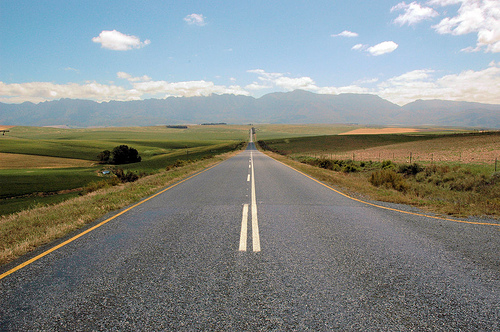
\includegraphics[width=0.5\textwidth]{photos/roadby_cornstaruk_flickr.jpg}
\end{center}
\end{Investigation}
  \label{m38791**end}
         \subsection*{Acceleration}
    \nopagebreak
            \label{m38794} $ \hspace{-5pt}\begin{array}{cccccccccccc}   
\includegraphics[width=0.75cm]{col11305.imgs/summary_fullmarks.png} &   
\includegraphics[width=0.75cm]{col11305.imgs/summary_video.png} &   \end{array} $ \hspace{2 pt}\raisebox{-5 pt}{} {(section shortcode: P10100 )} \par 
\Definition{ Acceleration } {Acceleration is the rate of change of velocity.} 
      \end{tabular*}
      \end{definition}
      \label{m38794*id67562}Acceleration (symbol $a$) is the rate of change of velocity. It is a measure of how fast the velocity of an object changes in time. If we have a change in velocity ($\Delta v$) over a time interval ($\Delta t$), then the acceleration ($a$) is defined as:\par 
      \label{m38794*id67610}\nopagebreak\noindent{}
        
    \begin{equation}
    \mathsf{acceleration}\phantom{\rule{4pt}{0ex}}\left(\mathsf{in}\phantom{\rule{4pt}{0ex}}\mathsf{m}\ensuremath{\cdot}{\mathsf{s}}^{-2}\right)=\frac{\mathsf{change}\phantom{\rule{4pt}{0ex}}\mathsf{in}\phantom{\rule{4pt}{0ex}}\mathsf{velocity}\phantom{\rule{4pt}{0ex}}\left(\mathsf{in}\phantom{\rule{4pt}{0ex}}\mathsf{m}\ensuremath{\cdot}{\mathsf{s}}^{-1}\right)}{\mathsf{change}\phantom{\rule{4pt}{0ex}}\mathsf{in}\phantom{\rule{4pt}{0ex}}\mathsf{time}\phantom{\rule{4pt}{0ex}}\left(\mathsf{in}\phantom{\rule{4pt}{0ex}}\mathsf{s}\right)}
      \end{equation}
      \label{m38794*id67742}\nopagebreak\noindent{}
        
    \begin{equation}
    a=\frac{\Delta v}{\Delta t}
      \end{equation}
      \label{m38794*id67769}Since velocity is a vector, acceleration is also a vector. Acceleration does not provide any information about a motion, but only about how the motion changes. It is not possible to tell how fast an object is moving or in which direction from the acceleration.\par 
      \label{m38794*id67775}Like velocity, acceleration can be negative or positive. We see that when the sign of the acceleration and the velocity are the same, the object is speeding up. If both velocity and acceleration are positive, the object is speeding up in a positive direction. If both velocity and acceleration are negative, the object is speeding up in a negative direction.
If velocity is positive and acceleration is negative, then the object is slowing down. Similarly, if the velocity is negative and the acceleration is positive the object is slowing down. This is illustrated in the following worked example.\par \vspace{-1cm}
\begin{wex}{Acceleration}
{A car accelerates uniformly from and initial velocity of 2 m$\cdot$s$^{-1}$ to a final velocity of 10 m$\cdot$s$^1$ in 8 seconds. It then slows down uniformly to a final velocity of 4 m$\cdot$s$^{-1}$ in 6 seconds. Calculate the acceleration of the car during the first 8 seconds and during the last 6 seconds.}
{
\westep{Identify what information is given and what is asked for:}
Consider the motion of the car in two parts: the first 8 seconds and the last 6 seconds.\\
\\
\begin{minipage}{0.5\textwidth}
\center{For the first 8 seconds:}
\begin{eqnarray*}
v_i &=& 2~\mathsf{m}\cdot \mathsf{s}^{-1}\\
v_f &=& 10~\mathsf{m}\cdot \mathsf{s}^{-1}\\
t_i &=& 0~\mathsf{s}\\
t_f &=& 8~\mathsf{s}
\end{eqnarray*}
\end{minipage}
\begin{minipage}{0.5\textwidth}
\center{For the last 6 seconds:}
\begin{eqnarray*}
v_i &=& 10~\mathsf{m}\cdot \mathsf{s}^{-1}\\
v_f &=& 4~\mathsf{m}\cdot \mathsf{s}^{-1}\\
t_i &=& 8~\mathsf{s}\\
t_f &=& 14~\mathsf{s}
\end{eqnarray*}
\end{minipage}\\

\westep{Calculate the acceleration.}
\begin{minipage}{0.5\textwidth}
\center{For the first 8 seconds:}
\begin{eqnarray*}
a &=& \frac{\Delta v}{\Delta t}\\
&=& \frac{10\textrm{ \ms} - 2\textrm{ \ms}}{8\textrm{ s} - 0\textrm{ s}}\\
&=& 1~\mathsf{m}\cdot \mathsf{s}^{-2}
\end{eqnarray*}
\end{minipage}
\begin{minipage}{0.5\textwidth}
\center{For the next 6 seconds:}
\begin{eqnarray*}
a &=& \frac{\Delta v}{\Delta t}\\
&=& \frac{4\textrm{ \ms} - 10\textrm{ \ms}}{14\textrm{ s} - 8\textrm{ s}}\\
&=& -1~\mathsf{m}\cdot \mathsf{s}^{-2}
\end{eqnarray*}
\end{minipage}\\
During the first 8 seconds the car had a positive acceleration. This means that its velocity increased. The velocity is positive so the car is speeding up.
During the next 6 seconds the car had a negative acceleration. This means that its velocity decreased. The velocity is positive so the car is slowing down.}
\end{wex}
    \noindent
\label{m38794*notfhsst!!!underscore!!!id1812}
\Tip{Acceleration does not tell us about the direction of the motion. Acceleration only tells us how the velocity changes.}
\Tip{Avoid the use of the word \textsl{deceleration} to refer to a negative acceleration. This word usually means \textsl{slowing down} and it is possible for an object to slow down with both a positive and negative acceleration, because the sign of the velocity of the object must also be taken into account to determine whether the body is slowing down or not.}
	\par
\label{m38794*secfhsst!!!underscore!!!id1815}
\begin{exercises}{Acceleration }
            \nopagebreak \noindent
      \label{m38794*id62523}\begin{enumerate}[noitemsep, label=\textbf{\arabic*}. ] 
            \label{m38794*uid78}\item An athlete is accelerating uniformly from an initial velocity of 0 m$\ensuremath{\cdot}$s${}^{-1}$to a final velocity of 4 m$\ensuremath{\cdot}$s${}^{-1}$in 2 seconds. Calculate his acceleration. Let the direction that the athlete is running in be the positive direction.\newline
\label{m38794*uid79}\item A bus accelerates uniformly from an initial velocity of 15 m$\ensuremath{\cdot}$s${}^{-1}$to a final velocity of 7~m$\ensuremath{\cdot}$s${}^{-1}$in 4 seconds. Calculate the acceleration of the bus. Let the direction of motion of the bus be the positive direction.\newline
\label{m38794*uid80}\item An aeroplane accelerates uniformly from an initial velocity of 200 m$\ensuremath{\cdot}$s${}^{-1}$to a velocity of 100 m$\ensuremath{\cdot}$s${}^{-1}$in 10 seconds. It then accelerates uniformly to a final velocity of 240 m$\ensuremath{\cdot}$s${}^{-1}$in 20 seconds. Let the direction of motion of the aeroplane be the positive direction.
\label{m38794*id68889}\begin{enumerate}[noitemsep, label=\textbf{\alph*}. ] 
            \label{m38794*uid81}\item Calculate the acceleration of the aeroplane during the first 10 seconds of the motion.
\label{m38794*uid82}\item Calculate the acceleration of the aeroplane during the next 14 seconds of its motion.
\end{enumerate}
                \end{enumerate}
  \label{m38794**end}
\par \raisebox{-5 pt}{
\includegraphics[width=0.5cm]{col11305.imgs/summary_www.png}} Find the answers with the shortcodes:
 \par \begin{tabular}[h]{cccccc}
 (1.) l1k  &  (2.) l10  &  (3.) l18  & \end{tabular}
\end{exercises}
\label{m38794*eip-307}The following video provides a summary of distance, velocity and acceleration. Note that in this video a different convention for writing units is used. You should not use this convention when writing units in physics.
    \setcounter{subfigure}{0}
	\begin{figure}[H] % horizontal\label{m38794*motion-1}
    \textnormal{Khan academy video on motion - 1}\vspace{.1in} \nopagebreak
  \label{m38794*yt-media1}\label{m38794*yt-video1}
            \raisebox{-5 pt}{ 
\includegraphics[width=0.5cm]{col11305.imgs/summary_www.png}} { (Video:  P10101 )}
      \vspace{2pt}
    \vspace{.1in}
 \end{figure}       \par 
%NTS CAPS says that instantaneous speed and velocity must only be covered now and not be covered where they currently are
         \section{Description of motion}
%NTS this section needs a formal project on acceleration
    \nopagebreak
            \label{m38795} $ \hspace{-5pt}\begin{array}{cccccccccccc}   
\includegraphics[width=0.75cm]{col11305.imgs/summary_fullmarks.png} &   
\includegraphics[width=0.75cm]{col11305.imgs/summary_simulation.png} &   \end{array} $ \hspace{2 pt}\raisebox{-5 pt}{} {(section shortcode: P10102 )} \par 
            \label{m38795*id68951}The purpose of this chapter is to describe motion, and now that we understand the definitions of displacement, distance, velocity, speed and acceleration, we are ready to start using these ideas to describe how an object is moving. There are many ways of describing motion:\par 
      \label{m38795*id68956}\begin{enumerate}[noitemsep, label=\textbf{\arabic*}. ] 
            \label{m38795*uid84}\item words
\label{m38795*uid85}\item diagrams
\label{m38795*uid86}\item graphs
\end{enumerate}
      \label{m38795*id68997}These methods will be described in this section.\par 
      \label{m38795*id69001}We will consider three types of motion: when the object is not moving (stationary object), when the object is moving at a constant velocity (uniform motion) and when the object is moving at a constant acceleration (motion at constant acceleration).\par 
      \label{m38795*uid87}
            \subsection*{Stationary Object}
            \nopagebreak
        \label{m38795*id69015}The simplest motion that we can come across is that of a stationary object. A stationary object does not move and so its position does not change, for as long as it is standing still.
An example of this situation is when someone is waiting for something without moving.
The person remains in the same position.\par 
        \label{m38795*id69021}Lesedi is waiting for a taxi. He is standing two metres from a stop street at $t$ = 0 s. After one minute, at $t$ = 60 $\mathsf{s}$, he is still 2 metres from the stop street and after two minutes, at $t$~=~120~$\mathsf{s}$, also 2 metres from the stop street. His position has not changed. His displacement is zero (because his position is the same), his velocity is zero (because his displacement is zero) and his acceleration is also zero (because his velocity is not changing).\par 
    \setcounter{subfigure}{0}
\begin{figure}[H]
\begin{center}
%Lesedi at t=0s. Stationary.
\scalebox{1} % Change this value to rescale the drawing.
{
\begin{pspicture}(0,-1.24)(8.404062,1.22)
\pspolygon[linewidth=0.04](4.5679913,1.2)(4.7965627,0.9714286)(4.7965627,0.62857145)(4.5679913,0.4)(4.225134,0.4)(3.9965625,0.62857145)(3.9965625,0.9714286)(4.225134,1.2)
\psline[linewidth=0.08cm](4.3765626,0.42)(4.3765626,-0.92)
\psline[linewidth=0.04cm,tbarsize=0.07055555cm 5.0]{|-|}(4.3565626,-0.88)(1.1965625,-0.9)
\usefont{T1}{ptm}{m}{n}
\rput(4.37,0.795){\footnotesize STOP}
\usefont{T1}{ptm}{m}{n}
\rput(2.671875,-1.09){2 m}
\usefont{T1}{ptm}{m}{n}
\rput(0.44859374,-0.09){t = 0 s}
\rput(0.44859374,-0.49){t = 60 s}
\rput(0.44859374,-0.89){t = 120 s}
\psellipse[linewidth=0.04,dimen=outer](1.1965625,0.39)(0.18,0.31)
\psline[linewidth=0.04cm](1.1965625,0.1)(1.1965625,-0.42)
\psline[linewidth=0.04cm](1.1965625,-0.4)(1.2765625,-0.7)
\psline[linewidth=0.04cm](1.2765625,-0.68)(1.2765625,-0.88)
\psline[linewidth=0.04cm](1.2765625,-0.86)(1.3365625,-0.86)
\psline[linewidth=0.04cm](1.1965625,-0.4)(1.1165625,-0.7)
\psline[linewidth=0.04cm](1.1165625,-0.7)(1.1165625,-0.9)
\psline[linewidth=0.04cm](1.1165625,-0.9)(1.0365624,-0.88)
\psline[linewidth=0.04cm](1.2165625,-0.02)(1.2565625,-0.28)
\psline[linewidth=0.04cm](1.2565625,-0.28)(1.2965626,-0.12)
\psline[linewidth=0.04cm](1.1965625,0.0)(1.1165625,-0.38)
\psline[linewidth=0.04cm](1.1165625,-0.38)(1.0765625,-0.18)
\psdots[dotsize=0.108](1.2565625,0.48)
\psdots[dotsize=0.108](1.1365625,0.48)
\pscustom[linewidth=0.04,fillstyle=solid]
{
\newpath
\moveto(1.0765625,0.32)
\lineto(1.1065625,0.29)
\curveto(1.1215625,0.275)(1.1615624,0.26)(1.1865625,0.26)
\curveto(1.2115625,0.26)(1.2515625,0.27)(1.2665625,0.28)
\curveto(1.2815624,0.29)(1.3015625,0.305)(1.3165625,0.32)
}
\pscustom[linewidth=0.04,fillstyle=solid]
{
\newpath
\moveto(1.3365625,0.5)
\lineto(1.3665625,0.49)
\curveto(1.3815625,0.485)(1.3865625,0.465)(1.3565625,0.42)
}
\pscustom[linewidth=0.04,fillstyle=solid]
{
\newpath
\moveto(1.0365624,0.52)
\lineto(1.0165625,0.49)
\curveto(1.0065625,0.475)(1.0065625,0.45)(1.0365624,0.42)
}
\psdots[dotsize=0.08](1.1965625,0.36)
\usefont{T1}{ptm}{m}{n}
\rput[l](6,0.81){displacement = 0 m}
\usefont{T1}{ptm}{m}{n}
\rput[l](6,0.23){velocity = 0 \ms}
\usefont{T1}{ptm}{m}{n}
\rput[l](6,-0.35){acceleration = 0 \mss}
\end{pspicture} 
}
\end{center}
\end{figure}      
        \label{m38795*id69081}We can now draw graphs of position vs. time ($x$ vs. $t$), velocity vs. time ($v$ vs. $t$) and acceleration vs. time ($a$ vs. $t$) for a stationary object. The graphs are shown in Figure~20.16.
Lesedi's position is 2~metres from the stop street. If the stop street is taken as the reference point, his position remains at 2~metres for 120~seconds. The graph is a horizontal line at 2~m.
The velocity and acceleration graphs are also shown. They are both horizontal lines on the $x$-axis. Since his position is not changing, his velocity is $0\phantom{\rule{2pt}{0ex}}\mathsf{m}\ensuremath{\cdot}\mathsf{s}{}^{-1}$ and since velocity is not changing, acceleration is $0\phantom{\rule{2pt}{0ex}}\mathsf{m}\ensuremath{\cdot}\mathsf{s}{}^{-2}$.\par 
    \setcounter{subfigure}{0}
\begin{figure}[H]
\begin{center}
\scalebox{1} % Change this value to rescale the drawing.
{
\begin{pspicture}(0,-2.3034375)(15.0207815,2.3034375)
\usefont{T1}{ptm}{m}{n}
\rput(9.671615,2.3734374){   }
\psline[linewidth=0.04cm,arrowsize=0.05291667cm 2.0,arrowlength=1.4,arrowinset=0.4]{->}(0.79578125,-1.1865625)(0.79578125,1.8134375)
\psline[linewidth=0.04cm,arrowsize=0.05291667cm 2.0,arrowlength=1.4,arrowinset=0.4]{->}(0.79578125,-1.1865625)(3.7957811,-1.1865625)
\psline[linewidth=0.04cm,arrowsize=0.05291667cm 2.0,arrowlength=1.4,arrowinset=0.4]{->}(5.795781,-1.1865625)(5.795781,1.8134375)
\psline[linewidth=0.04cm,arrowsize=0.05291667cm 2.0,arrowlength=1.4,arrowinset=0.4]{->}(5.795781,-1.1865625)(8.795781,-1.1865625)
\psline[linewidth=0.04cm,arrowsize=0.05291667cm 2.0,arrowlength=1.4,arrowinset=0.4]{->}(10.795781,-1.1865625)(10.795781,1.8134375)
\psline[linewidth=0.04cm,arrowsize=0.05291667cm 2.0,arrowlength=1.4,arrowinset=0.4]{->}(10.795781,-1.1865625)(13.795781,-1.1865625)
\psline[linewidth=0.09cm](10.795781,-1.1865625)(12.795781,-1.1865625)
\psline[linewidth=0.09cm](5.795781,-1.1865625)(7.795781,-1.1865625)
\psline[linewidth=0.09cm](0.79578125,0.8134375)(2.7957811,0.8134375)
\usefont{T1}{ptm}{m}{n}
\rput(1.7615625,-1.4765625){60}
\usefont{T1}{ptm}{m}{n}
\rput(2.8382812,-1.4765625){120}
\usefont{T1}{ptm}{m}{n}
\rput(0.574375,0.8234375){2}
\usefont{T1}{ptm}{m}{n}
\rput(0.54265624,-0.1765625){1}
\usefont{T1}{ptm}{m}{n}
\rput(0.5728125,-1.2765625){0}
\usefont{T1}{ptm}{m}{n}
\rput(7.838281,-1.4765625){120}
\usefont{T1}{ptm}{m}{n}
\rput(12.738281,-1.4765625){120}
\psline[linewidth=0.04cm](1.7957813,-1.0865625)(1.7957813,-1.1865625)
\psline[linewidth=0.04cm](2.7957811,-1.0865625)(2.7957811,-1.1865625)
\psline[linewidth=0.04cm](6.795781,-1.0865625)(6.795781,-1.1865625)
\psline[linewidth=0.04cm](7.795781,-1.0865625)(7.795781,-1.1865625)
\psline[linewidth=0.04cm](11.795781,-1.0865625)(11.795781,-1.1865625)
\psline[linewidth=0.04cm](12.795781,-1.0865625)(12.795781,-1.1865625)
\psline[linewidth=0.04cm](0.69578123,-0.1865625)(0.8957813,-0.1865625)
\psline[linewidth=0.04cm](0.69578123,0.8134375)(0.79578125,0.8134375)
\usefont{T1}{ptm}{m}{n}
\rput(4.4365625,-1.1765625){time (s)}
\usefont{T1}{ptm}{m}{n}
\rput(9.436563,-1.1765625){time (s)}
\usefont{T1}{ptm}{m}{n}
\rput(14.436563,-1.1765625){time (s)}
\usefont{T1}{ptm}{m}{n}
\rput{-270.0}(0.571875,0.2365625){\rput(0.16890626,0.4234375){position $x$ (m)}}
\usefont{T1}{ptm}{m}{n}
\rput{-270.0}(5.9035935,-5.0960937){\rput(5.496719,0.4234375){velocity $v$ (\ms)}}
\usefont{T1}{ptm}{m}{n}
\rput{-270.0}(10.958906,-10.150469){\rput(10.541875,0.4234375){acceleration $a$ (\mss)}}
\usefont{T1}{ptm}{m}{n}
\rput(5.6728125,-1.2765625){0}
\usefont{T1}{ptm}{m}{n}
\rput(10.672812,-1.2765625){0}
\usefont{T1}{ptm}{m}{n}
\rput(6.7615623,-1.4765625){60}
\usefont{T1}{ptm}{m}{n}
\rput(11.761562,-1.4765625){60}
\usefont{T1}{ptm}{m}{n}
\rput(1.9809375,-2.0765624){(a)}
\usefont{T1}{ptm}{m}{n}
\rput(6.9909377,-2.0765624){(b)}
\usefont{T1}{ptm}{m}{n}
\rput(11.980938,-2.0765624){(c)}
\psline[linewidth=0.04cm,linestyle=dashed,dash=0.16cm 0.16cm](2.7957811,0.8134375)(2.7957811,-1.0865625)
\end{pspicture} 
}
\caption{Graphs for a stationary object (a) position vs. time (b) velocity vs. time (c) acceleration vs. time.}
\label{fig:pr:stationary}
\end{center}
\end{figure}      
\par
\Definition{ Gradient } {The gradient of a line can be calculated by dividing the change in the $y$-value by the change in the $x$-value. $m = \frac{\Delta y}{\Delta x}$ \par  } 
        \label{m38795*id69281}Since we know that velocity is the rate of change of position, we can confirm the value for the velocity vs. time graph, by calculating the gradient of the $x$ vs. $t$ graph.\par 
\label{m38795*notfhsst!!!underscore!!!id1870}
\Tip{The gradient of a position vs. time graph gives the velocity.}
	\par
        \label{m38795*id69310}If we calculate the gradient of the $x$ vs. $t$ graph for a stationary object we get:\par 
        \label{m38795*id69332}\nopagebreak\noindent{}
    \begin{equation}
    \begin{array}{cccc}\hfill v& =& \frac{\Delta x}{\Delta t}\hfill & \\ & =& \frac{{x}_{f}-{x}_{i}}{{t}_{f}-{t}_{i}}\hfill & \\ & =& \frac{2\phantom{\rule{3.33333pt}{0ex}}\mathsf{m}-2\phantom{\rule{3.33333pt}{0ex}}\mathsf{m}}{120\phantom{\rule{3.33333pt}{0ex}}\mathsf{s}-60\phantom{\rule{3.33333pt}{0ex}}\mathsf{s}}\hfill & \left(\mathsf{initial\; position}=\mathsf{final\; position}\right)\hfill \\ & =& 0\phantom{\rule{4pt}{0ex}}\phantom{\rule{0.166667em}{0ex}}\mathsf{m}\ensuremath{\cdot}{\mathsf{s}}^{-1}\hfill & \left(\mathsf{for\; the\; time\; that\; Lesedi\; is\; stationary}\phantom{\rule{2pt}{0ex}}\right)\hfill \end{array}
      \end{equation}
        \label{m38795*id69558}Similarly, we can confirm the value of the acceleration by calculating the gradient of the velocity vs. time graph.\par 
\label{m38795*notfhsst!!!underscore!!!id2005}
\Tip{The gradient of a velocity vs. time graph gives the acceleration.}
	\par
        \label{m38795*id69571}If we calculate the gradient of the $v$ vs. $t$ graph for a stationary object we get:\par 
        \label{m38795*id69594}\nopagebreak\noindent{}
          
    \begin{equation}
    \begin{array}{ccc}\hfill a& =& \frac{\Delta v}{\Delta t}\hfill \\ & =& \frac{{v}_{f}-{v}_{i}}{{t}_{f}-{t}_{i}}\hfill \\ & =& \frac{0\phantom{\rule{4pt}{0ex}}\phantom{\rule{0.166667em}{0ex}}\mathsf{m}\ensuremath{\cdot}{\mathsf{s}}^{-1}-0\phantom{\rule{4pt}{0ex}}\phantom{\rule{0.166667em}{0ex}}\mathsf{m}\ensuremath{\cdot}{\mathsf{s}}^{-1}}{120\phantom{\rule{3.33333pt}{0ex}}\mathsf{s}-60\phantom{\rule{3.33333pt}{0ex}}\mathsf{s}}\hfill \\ & =& 0\phantom{\rule{4pt}{0ex}}\phantom{\rule{0.166667em}{0ex}}\mathsf{m}\ensuremath{\cdot}{\mathsf{s}}^{-2}\hfill \end{array}
      \end{equation}
        \label{m38795*id69809}Additionally, because the velocity vs. time graph is related to the position vs. time graph, we can use the area under the velocity vs. time graph to calculate the displacement of an object.\par 
\label{m38795*notfhsst!!!underscore!!!id2134}
\Tip{The area under the velocity vs. time graph gives the displacement.}
	\par
        \label{m38795*id69821}The displacement of the object is given by the area under the graph, which is $0\phantom{\rule{2pt}{0ex}}\mathsf{m}$. This is obvious, because the object is not moving.\par 
      \label{m38795*uid90}
            \subsection*{Motion at Constant Velocity}
            \nopagebreak
        \label{m38795*id69835}Motion at a constant velocity or \textsl{uniform motion} means that the position of the object is changing at the same rate.\par 
        \label{m38795*id69845}Assume that Lesedi takes $100\phantom{\rule{2pt}{0ex}}\mathsf{s}$ to walk the $100\phantom{\rule{2pt}{0ex}}\mathsf{m}$ to the taxi-stop every morning. If we assume that Lesedi's house is the origin, then Lesedi's velocity is:\par 
        \label{m38795*id69850}\nopagebreak\noindent{}
          
    \begin{equation}
    \begin{array}{ccc}\hfill v& =& \frac{\Delta x}{\Delta t}\hfill \\ & =& \frac{{x}_{f}-{x}_{i}}{{t}_{f}-{t}_{i}}\hfill \\ & =& \frac{100\phantom{\rule{4pt}{0ex}}\mathsf{m}-0\phantom{\rule{4pt}{0ex}}\mathsf{m}}{100\phantom{\rule{4pt}{0ex}}\mathsf{s}-0\phantom{\rule{4pt}{0ex}}\mathsf{s}}\hfill \\ & =& 1\phantom{\rule{4pt}{0ex}}\phantom{\rule{0.166667em}{0ex}}\mathsf{m}\ensuremath{\cdot}{\mathsf{s}}^{-1}\hfill \end{array}
      \end{equation}
        \label{m38795*id70029}Lesedi's velocity is 1 m$\ensuremath{\cdot}$s${}^{-1}$. This means that he walked $1\phantom{\rule{2pt}{0ex}}\mathsf{m}$ in the first second, another metre in the second second, and another in the third second, and so on. For example, after $50\phantom{\rule{2pt}{0ex}}\mathsf{s}$ he will be $50\phantom{\rule{2pt}{0ex}}\mathsf{m}$ from home. His position increases by $1\phantom{\rule{2pt}{0ex}}\mathsf{m}$ every $1\phantom{\rule{2pt}{0ex}}\mathsf{s}$. A diagram of Lesedi's position is shown in Figure~\ref{fig:pr:diagram:uniform}.\par 
    \setcounter{subfigure}{0}
	\begin{figure}[H] % horizontal\label{m38795*uid91}
\begin{center}
\scalebox{1} % Change this value to rescale the drawing.
{
\begin{pspicture}(0,-1.57375)(9.02,1.53375)
\psline[linewidth=0.04cm,arrowsize=0.05291667cm 2.0,arrowlength=1.4,arrowinset=0.4]{->}(2.0,-0.46625)(9.0,-0.46625)
\psframe[linewidth=0.04,dimen=outer](2.0,0.53375)(0.0,-0.46625)
\pstriangle[linewidth=0.04,dimen=outer](1.0,0.53375)(2.0,1.0)
\psframe[linewidth=0.04,dimen=outer](1.2,0.23375)(0.8,-0.46625)
\psframe[linewidth=0.04,dimen=outer](1.8,0.23375)(1.4,-0.06625)
\psframe[linewidth=0.04,dimen=outer](0.6,0.23375)(0.2,-0.06625)
\psellipse[linewidth=0.04,dimen=outer](2.15,0.53375)(0.15,0.2)
\psline[linewidth=0.04cm](2.1,0.33375)(2.1,0.33375)
\psline[linewidth=0.051999997cm](2.14,0.37375)(2.14,-0.02625)
\psline[linewidth=0.04cm](2.14,-0.02625)(2.24,-0.24625)
\psline[linewidth=0.04cm](2.24,-0.24625)(2.2,-0.42625)
\psline[linewidth=0.04cm](2.2,-0.42625)(2.3,-0.42625)
\psline[linewidth=0.04cm](2.12,-0.00625)(2.1,-0.26625)
\psline[linewidth=0.04cm](2.1,-0.26625)(2.02,-0.42625)
\psline[linewidth=0.04cm](2.02,-0.42625)(2.12,-0.42625)
\psline[linewidth=0.04cm](2.12,0.27375)(2.04,0.03375)
\psline[linewidth=0.04cm](2.04,0.03375)(2.22,0.15375)
\psline[linewidth=0.04cm](2.12,0.21375)(2.24,-0.02625)
\psline[linewidth=0.04cm](2.24,-0.02625)(2.32,0.03375)
\psdots[dotsize=0.04](2.2,0.59375)
\pscustom[linewidth=0.04]
{
\newpath
\moveto(2.12,0.51375)
\lineto(2.17,0.47375)
\curveto(2.195,0.45375)(2.225,0.43875)(2.24,0.45375)
}
\pscustom[linewidth=0.04]
{
\newpath
\moveto(2.24,0.69375)
\lineto(2.19,0.70375)
\curveto(2.165,0.70875)(2.12,0.70875)(2.1,0.70375)
\curveto(2.08,0.69875)(2.05,0.67875)(2.04,0.66375)
\curveto(2.03,0.64875)(2.015,0.62875)(2.0,0.61375)
}
\pscustom[linewidth=0.04]
{
\newpath
\moveto(2.0,0.61375)
\lineto(2.03,0.64375)
\curveto(2.045,0.65875)(2.08,0.67875)(2.1,0.68375)
\curveto(2.12,0.68875)(2.165,0.69375)(2.19,0.69375)
\curveto(2.215,0.69375)(2.245,0.68375)(2.26,0.65375)
}
\pscustom[linewidth=0.04]
{
\newpath
\moveto(2.14,0.71375)
\lineto(2.1,0.67375)
\curveto(2.08,0.65375)(2.055,0.61875)(2.04,0.57375)
}
\usefont{T1}{ptm}{m}{n}
\rput[l](8,-1.05625){$x$ = 100 m}
\usefont{T1}{ptm}{m}{n}
\rput[l](2,-0.73625){t = 0 s}
\usefont{T1}{ptm}{m}{n}
\rput[l](5,-0.73625){t = 50 s}
\usefont{T1}{ptm}{m}{n}
\rput[l](8,-0.73625){t = 100 s}
\usefont{T1}{ptm}{m}{n}
\rput[l](5,-1.05625){$x$ = 50 m}
\usefont{T1}{ptm}{m}{n}
\rput[l](2,-1.05625){$x$ = 0 m}
\psline[linewidth=0.04cm,linestyle=dashed,dash=0.16cm 0.16cm](5.0,1.07375)(5.0,-0.44625)
\psline[linewidth=0.04cm,linestyle=dashed,dash=0.16cm 0.16cm](7.98,1.05375)(7.98,-0.46625)
\psellipse[linewidth=0.04,dimen=outer](5.17,0.51375)(0.15,0.2)
\psline[linewidth=0.04cm](5.12,0.31375)(5.12,0.31375)
\psline[linewidth=0.051999997cm](5.16,0.35375)(5.16,-0.04625)
\psline[linewidth=0.04cm](5.16,-0.04625)(5.26,-0.26625)
\psline[linewidth=0.04cm](5.26,-0.26625)(5.22,-0.44625)
\psline[linewidth=0.04cm](5.14,-0.02625)(5.12,-0.28625)
\psline[linewidth=0.04cm](5.12,-0.28625)(5.04,-0.44625)
\psline[linewidth=0.04cm](5.14,0.25375)(5.06,0.01375)
\psline[linewidth=0.04cm](5.06,0.01375)(5.24,0.13375)
\psline[linewidth=0.04cm](5.14,0.19375)(5.26,-0.04625)
\psline[linewidth=0.04cm](5.26,-0.04625)(5.34,0.01375)
\psdots[dotsize=0.04](5.22,0.57375)
\pscustom[linewidth=0.04]
{
\newpath
\moveto(5.14,0.49375)
\lineto(5.19,0.45375)
\curveto(5.215,0.43375)(5.245,0.41875)(5.26,0.43375)
}
\pscustom[linewidth=0.04]
{
\newpath
\moveto(5.26,0.67375)
\lineto(5.21,0.68375)
\curveto(5.185,0.68875)(5.14,0.68875)(5.12,0.68375)
\curveto(5.1,0.67875)(5.07,0.65875)(5.06,0.64375)
\curveto(5.05,0.62875)(5.035,0.60875)(5.02,0.59375)
}
\pscustom[linewidth=0.04]
{
\newpath
\moveto(5.02,0.59375)
\lineto(5.05,0.62375)
\curveto(5.065,0.63875)(5.1,0.65875)(5.12,0.66375)
\curveto(5.14,0.66875)(5.185,0.67375)(5.21,0.67375)
\curveto(5.235,0.67375)(5.265,0.66375)(5.28,0.63375)
}
\pscustom[linewidth=0.04]
{
\newpath
\moveto(5.16,0.69375)
\lineto(5.12,0.65375)
\curveto(5.1,0.63375)(5.075,0.59875)(5.06,0.55375)
}
\psellipse[linewidth=0.04,dimen=outer](8.13,0.55375)(0.15,0.2)
\psline[linewidth=0.04cm](8.08,0.35375)(8.08,0.35375)
\psline[linewidth=0.051999997cm](8.12,0.39375)(8.12,-0.00625)
\psline[linewidth=0.04cm](8.1,0.01375)(8.08,-0.24625)
\psline[linewidth=0.04cm](8.1,0.29375)(8.02,0.05375)
\psline[linewidth=0.04cm](8.02,0.05375)(8.2,0.17375)
\psline[linewidth=0.04cm](8.1,0.23375)(8.22,-0.00625)
\psline[linewidth=0.04cm](8.22,-0.00625)(8.3,0.05375)
\psdots[dotsize=0.04](8.18,0.61375)
\pscustom[linewidth=0.04]
{
\newpath
\moveto(8.1,0.53375)
\lineto(8.15,0.49375)
\curveto(8.175,0.47375)(8.205,0.45875)(8.22,0.47375)
}
\pscustom[linewidth=0.04]
{
\newpath
\moveto(8.22,0.71375)
\lineto(8.17,0.72375)
\curveto(8.145,0.72875)(8.1,0.72875)(8.08,0.72375)
\curveto(8.06,0.71875)(8.03,0.69875)(8.02,0.68375)
\curveto(8.01,0.66875)(7.995,0.64875)(7.98,0.63375)
}
\pscustom[linewidth=0.04]
{
\newpath
\moveto(7.98,0.63375)
\lineto(8.01,0.66375)
\curveto(8.025,0.67875)(8.06,0.69875)(8.08,0.70375)
\curveto(8.1,0.70875)(8.145,0.71375)(8.17,0.71375)
\curveto(8.195,0.71375)(8.225,0.70375)(8.24,0.67375)
}
\pscustom[linewidth=0.04]
{
\newpath
\moveto(8.12,0.73375)
\lineto(8.08,0.69375)
\curveto(8.06,0.67375)(8.035,0.63875)(8.02,0.59375)
}
\psline[linewidth=0.04cm,linestyle=dashed,dash=0.16cm 0.16cm](8.14,-0.44625)(8.22,-0.44625)
\psline[linewidth=0.04cm,linestyle=dashed,dash=0.16cm 0.16cm](8.02,-0.44625)(8.1,-0.44625)
\psline[linewidth=0.04cm](8.12,-0.00625)(8.22,-0.22625)
\psline[linewidth=0.04cm](8.08,-0.22625)(8.02,-0.44625)
\psline[linewidth=0.04cm](8.22,-0.20625)(8.14,-0.44625)
\psline[linewidth=0.04cm](5.02,-0.42625)(5.12,-0.42625)
\psline[linewidth=0.04cm](5.2,-0.42625)(5.28,-0.42625)
\usefont{T1}{ptm}{m}{n}
\rput[l](5,-1.37625){$v$ = 1\ms}
\usefont{T1}{ptm}{m}{n}
\rput[l](8,-1.39625){$v$ = 1\ms}
\end{pspicture} 
}
\end{center}
\caption{Diagram showing Lesedi's motion at a constant velocity of 1 \ms}
\label{fig:pr:diagram:uniform}
\end{figure}     
        \label{m38795*id70106}We can now draw graphs of position vs.time ($x$ vs. $t$), velocity vs.time ($v$ vs. $t$) and acceleration vs.time ($a$ vs. $t$) for Lesedi moving at a constant velocity. The graphs are shown in Figure~\ref{fig:pr:uniform}. \\ 
    \setcounter{subfigure}{0}
\begin{figure}[H]
\begin{center}
\scalebox{1} % Change this value to rescale the drawing.
{
\begin{pspicture}(0,-2.3034375)(15.220781,2.3034375)
\definecolor{color1158b}{rgb}{0.8,0.8,0.8}
\usefont{T1}{ptm}{m}{n}
\rput(9.871614,2.3734374){   }
\psline[linewidth=0.04cm,arrowsize=0.05291667cm 2.0,arrowlength=1.4,arrowinset=0.4]{->}(0.99578124,-1.1865625)(0.99578124,1.8134375)
\psline[linewidth=0.04cm,arrowsize=0.05291667cm 2.0,arrowlength=1.4,arrowinset=0.4]{->}(0.99578124,-1.1865625)(3.9957812,-1.1865625)
\psline[linewidth=0.04cm,arrowsize=0.05291667cm 2.0,arrowlength=1.4,arrowinset=0.4]{->}(5.9957814,-1.1865625)(5.9957814,1.8134375)
\psline[linewidth=0.04cm,arrowsize=0.05291667cm 2.0,arrowlength=1.4,arrowinset=0.4]{->}(5.9957814,-1.1865625)(8.995781,-1.1865625)
\psline[linewidth=0.04cm,arrowsize=0.05291667cm 2.0,arrowlength=1.4,arrowinset=0.4]{->}(10.995781,-1.1865625)(10.995781,1.8134375)
\psline[linewidth=0.04cm,arrowsize=0.05291667cm 2.0,arrowlength=1.4,arrowinset=0.4]{->}(10.995781,-1.1865625)(13.995781,-1.1865625)
\psline[linewidth=0.09cm](10.995781,-1.1865625)(12.995781,-1.1865625)
\psline[linewidth=0.09cm](5.9957814,-0.1865625)(7.9957814,-0.1865625)
\psline[linewidth=0.09cm](0.99578124,-1.1865625)(2.9957812,0.8134375)
\usefont{T1}{ptm}{m}{n}
\rput(1.9607812,-1.4765625){50}
\usefont{T1}{ptm}{m}{n}
\rput(3.0382812,-1.4765625){100}
\usefont{T1}{ptm}{m}{n}
\rput(0.53828126,0.8234375){100}
\usefont{T1}{ptm}{m}{n}
\rput(0.66078126,-0.1765625){50}
\usefont{T1}{ptm}{m}{n}
\rput(0.7728125,-1.2765625){0}
\usefont{T1}{ptm}{m}{n}
\rput(8.038281,-1.4765625){100}
\usefont{T1}{ptm}{m}{n}
\rput(12.938281,-1.4765625){100}
\psline[linewidth=0.04cm](1.9957813,-1.0865625)(1.9957813,-1.1865625)
\psline[linewidth=0.04cm](2.9957812,-1.0865625)(2.9957812,-1.1865625)
\psline[linewidth=0.04cm](6.9957814,-1.0865625)(6.9957814,-1.1865625)
\psline[linewidth=0.04cm](7.9957814,-1.0865625)(7.9957814,-1.1865625)
\psline[linewidth=0.04cm](11.995781,-1.0865625)(11.995781,-1.1865625)
\psline[linewidth=0.04cm](12.995781,-1.0865625)(12.995781,-1.1865625)
\psline[linewidth=0.04cm](0.8957813,-0.1865625)(1.0957812,-0.1865625)
\psline[linewidth=0.04cm](0.8957813,0.8134375)(0.99578124,0.8134375)
\usefont{T1}{ptm}{m}{n}
\rput(4.6365623,-1.1765625){time (s)}
\usefont{T1}{ptm}{m}{n}
\rput(9.636562,-1.1765625){time (s)}
\usefont{T1}{ptm}{m}{n}
\rput(14.636562,-1.1765625){time (s)}
\usefont{T1}{ptm}{m}{n}
\rput{-270.0}(0.571875,0.2365625){\rput(0.16890626,0.4234375){position $x$ (m)}}
\usefont{T1}{ptm}{m}{n}
\rput{-270.0}(5.8035936,-4.9960938){\rput(5.396719,0.4234375){velocity $v$ (\ms)}}
\usefont{T1}{ptm}{m}{n}
\rput{-270.0}(11.158906,-10.350469){\rput(10.741875,0.4234375){acceleration $a$ (\mss)}}
\usefont{T1}{ptm}{m}{n}
\rput(5.8728123,-1.2765625){0}
\usefont{T1}{ptm}{m}{n}
\rput(10.872812,-1.2765625){0}
\usefont{T1}{ptm}{m}{n}
\rput(6.960781,-1.4765625){50}
\usefont{T1}{ptm}{m}{n}
\rput(11.960781,-1.4765625){50}
\usefont{T1}{ptm}{m}{n}
\rput(2.1809375,-2.0765624){(a)}
\usefont{T1}{ptm}{m}{n}
\rput(7.1909375,-2.0765624){(b)}
\usefont{T1}{ptm}{m}{n}
\rput(12.180938,-2.0765624){(c)}
\psline[linewidth=0.04cm,linestyle=dashed,dash=0.16cm 0.16cm](2.9957812,0.8134375)(2.9957812,-1.0865625)
\usefont{T1}{ptm}{m}{n}
\rput(5.742656,-0.1765625){1}
\psline[linewidth=0.04cm](5.895781,-0.1865625)(6.0957813,-0.1865625)
\psline[linewidth=0.04cm,linestyle=dashed,dash=0.16cm 0.16cm](2.8957813,0.8134375)(0.99578124,0.8134375)
\psline[linewidth=0.04cm,linestyle=dashed,dash=0.16cm 0.16cm](7.9957814,-0.1865625)(7.9957814,-1.1865625)
\psframe[linewidth=0.02,linecolor=color1158b,dimen=outer,fillstyle=solid,fillcolor=color1158b](7.9757814,-0.2265625)(6.0157814,-1.1465625)
\psline[linewidth=0.03cm,linestyle=dashed,dash=0.16cm 0.16cm](2.5757813,0.3534375)(2.5757813,-0.5865625)
\psline[linewidth=0.03cm,linestyle=dashed,dash=0.16cm 0.16cm](2.5757813,-0.5865625)(1.6357813,-0.5865625)
\usefont{T1}{ptm}{m}{n}
\rput[l](2.7,-0.1365625){$\Delta$x}
\usefont{T1}{ptm}{m}{n}
\rput(2.2054687,-0.7315625){\footnotesize $\Delta$t}
\end{pspicture} 
}
\caption{Graphs for motion at constant velocity (a) position vs. time (b) velocity vs. time (c) acceleration vs. time. The area of the shaded portion in the $v$ vs. $t$ graph corresponds to the object's displacement.}
\label{fig:pr:uniform}
\end{center}
\end{figure}      
        \label{m38795*id70200}In the evening Lesedi walks $100\phantom{\rule{2pt}{0ex}}\mathsf{m}$ from the bus stop to his house in $100\phantom{\rule{2pt}{0ex}}\mathsf{s}$. Assume that Lesedi's house is the origin. The following graphs can be drawn to describe the motion.\par 
    \setcounter{subfigure}{0}
\begin{figure}[H]
\begin{center}
\scalebox{1} % Change this value to rescale the drawing.
{
\begin{pspicture}(0,-2.3034375)(15.220781,2.3034375)
\definecolor{color1158b}{rgb}{0.8,0.8,0.8}
\usefont{T1}{ptm}{m}{n}
\rput(9.871614,2.3734374){   }
\psline[linewidth=0.04cm,arrowsize=0.05291667cm 2.0,arrowlength=1.4,arrowinset=0.4]{->}(0.99578124,-1.1865625)(0.99578124,1.8134375)
\psline[linewidth=0.04cm,arrowsize=0.05291667cm 2.0,arrowlength=1.4,arrowinset=0.4]{->}(0.99578124,-1.1865625)(3.9957812,-1.1865625)
\psline[linewidth=0.04cm,arrowsize=0.05291667cm 2.0,arrowlength=1.4,arrowinset=0.4]{<->}(6.0110865,1.8133594)(5.980476,-1.1864845)
\psline[linewidth=0.04cm,arrowsize=0.05291667cm 2.0,arrowlength=1.4,arrowinset=0.4]{->}(5.9957814,0.8134375)(8.995781,0.8134375)
\psline[linewidth=0.04cm,arrowsize=0.05291667cm 2.0,arrowlength=1.4,arrowinset=0.4]{->}(10.995781,-1.1865625)(10.995781,1.8134375)
\psline[linewidth=0.04cm,arrowsize=0.05291667cm 2.0,arrowlength=1.4,arrowinset=0.4]{->}(10.995781,-1.1865625)(13.995781,-1.1865625)
\psline[linewidth=0.09cm](10.995781,-1.1865625)(12.995781,-1.1865625)
\psline[linewidth=0.09cm](5.9957814,-0.1865625)(7.9957814,-0.1865625)
\psline[linewidth=0.09cm](0.97578126,0.8134375)(2.9957812,-1.1865625)
\usefont{T1}{ptm}{m}{n}
\rput(1.9607812,-1.4765625){50}
\usefont{T1}{ptm}{m}{n}
\rput(3.0382812,-1.4765625){100}
\usefont{T1}{ptm}{m}{n}
\rput(0.53828126,0.8234375){100}
\usefont{T1}{ptm}{m}{n}
\rput(0.66078126,-0.1765625){50}
\usefont{T1}{ptm}{m}{n}
\rput(0.7728125,-1.2765625){0}
\usefont{T1}{ptm}{m}{n}
\rput(7.938281,1.0234375){100}
\usefont{T1}{ptm}{m}{n}
\rput(12.938281,-1.4765625){100}
\psline[linewidth=0.04cm](1.9957813,-1.0865625)(1.9957813,-1.1865625)
\psline[linewidth=0.04cm](2.9957812,-1.0865625)(2.9957812,-1.1865625)
\psline[linewidth=0.04cm](6.9957814,0.9134375)(6.9957814,0.8134375)
\psline[linewidth=0.04cm](7.9957814,0.9134375)(7.9957814,0.8134375)
\psline[linewidth=0.04cm](11.995781,-1.0865625)(11.995781,-1.1865625)
\psline[linewidth=0.04cm](12.995781,-1.0865625)(12.995781,-1.1865625)
\psline[linewidth=0.04cm](0.8957813,-0.1865625)(1.0957812,-0.1865625)
\psline[linewidth=0.04cm](0.8957813,0.8134375)(0.99578124,0.8134375)
\usefont{T1}{ptm}{m}{n}
\rput(4.6365623,-1.1765625){time (s)}
\usefont{T1}{ptm}{m}{n}
\rput(9.536563,0.8234375){time (s)}
\usefont{T1}{ptm}{m}{n}
\rput(14.636562,-1.1765625){time (s)}
\usefont{T1}{ptm}{m}{n}
\rput{-270.0}(0.571875,0.2365625){\rput(0.16890626,0.4234375){position $x$ (m)}}
\usefont{T1}{ptm}{m}{n}
\rput{-270.0}(5.8035936,-4.9960938){\rput(5.396719,0.4234375){velocity $v$ (\ms)}}
\usefont{T1}{ptm}{m}{n}
\rput{-270.0}(11.158906,-10.350469){\rput(10.741875,0.4234375){acceleration $a$ (\mss)}}
\usefont{T1}{ptm}{m}{n}
\rput(5.7728124,0.8234375){0}
\usefont{T1}{ptm}{m}{n}
\rput(10.872812,-1.2765625){0}
\usefont{T1}{ptm}{m}{n}
\rput(6.960781,1.0234375){50}
\usefont{T1}{ptm}{m}{n}
\rput(11.960781,-1.4765625){50}
\usefont{T1}{ptm}{m}{n}
\rput(2.1809375,-2.0765624){(a)}
\usefont{T1}{ptm}{m}{n}
\rput(7.1909375,-2.0765624){(b)}
\usefont{T1}{ptm}{m}{n}
\rput(12.180938,-2.0765624){(c)}
\usefont{T1}{ptm}{m}{n}
\rput(5.7164063,-0.1765625){-1}
\psline[linewidth=0.04cm](5.895781,-0.1865625)(6.0957813,-0.1865625)
\psline[linewidth=0.04cm,linestyle=dashed,dash=0.16cm 0.16cm](7.9957814,0.8134375)(7.9957814,-0.1865625)
\psframe[linewidth=0.02,linecolor=color1158b,dimen=outer,fillstyle=solid,fillcolor=color1158b](7.9757814,0.7734375)(6.0157814,-0.1465625)
\psline[linewidth=0.03cm,linestyle=dashed,dash=0.16cm 0.16cm](2.5757813,0.1534375)(2.5757813,-0.7865625)
\psline[linewidth=0.03cm,linestyle=dashed,dash=0.16cm 0.16cm](2.5757813,0.2134375)(1.6357813,0.2134375)
\usefont{T1}{ptm}{m}{n}
\rput(2.7920313,-0.2315625){\footnotesize $\Delta$x}
\usefont{T1}{ptm}{m}{n}
\rput(2.2854688,0.3684375){\footnotesize $\Delta$t}
\end{pspicture} 
}
\caption{Graphs for motion with a constant negative velocity (a) position vs. time (b) velocity vs. time (c) acceleration vs. time. The area of the shaded portion in the $v$ vs.$t$ graph corresponds to the object's displacement.}
\label{fig:pr:uniform:negative}
\end{center}
\end{figure}      
        \label{m38795*id70236}We see that the $v$ vs. $t$ graph is a horisontal line. If the velocity vs. time graph is a horisontal line, it means that the velocity is \textsl{constant} (not changing). Motion at a constant velocity is known as \textsl{uniform motion}.\par 
        \label{m38795*id70269}We can use the $x$ vs. $t$ to calculate the velocity by finding the gradient of the line.\par 
        \label{m38795*id70291}\nopagebreak\noindent{}
          
    \begin{equation}
    \begin{array}{ccc}\hfill v& =& \frac{\Delta x}{\Delta t}\hfill \\ & =& \frac{{x}_{f}-{x}_{i}}{{t}_{f}-{t}_{i}}\hfill \\ & =& \frac{0\phantom{\rule{3.33333pt}{0ex}}\mathsf{m}-100\phantom{\rule{3.33333pt}{0ex}}\mathsf{m}}{100\phantom{\rule{3.33333pt}{0ex}}\mathsf{s}-0\phantom{\rule{3.33333pt}{0ex}}\mathsf{s}}\hfill \\ & =& -1\phantom{\rule{4pt}{0ex}}\phantom{\rule{0.166667em}{0ex}}\mathsf{m}\ensuremath{\cdot}{\mathsf{s}}^{-1}\hfill \end{array}
      \end{equation}
        \label{m38795*id70472}Lesedi has a velocity of $-1\phantom{\rule{2pt}{0ex}}\mathsf{m}\ensuremath{\cdot}\mathsf{s}{}^{-1}$, or $1\phantom{\rule{2pt}{0ex}}\mathsf{m}\ensuremath{\cdot}\mathsf{s}{}^{-1}$ towards his house. You will notice that the $v$~vs.~$t$ graph is a horisontal line corresponding to a velocity of $-1\phantom{\rule{2pt}{0ex}}\mathsf{m}\ensuremath{\cdot}\mathsf{s}{}^{-1}$. The horizontal line means that the velocity stays the same (remains constant) during the motion. This is uniform velocity.\par 
        \label{m38795*id70573}We can use the $v$ vs. $t$ to calculate the acceleration by finding the gradient of the line.\par 
        \label{m38795*id70595}\nopagebreak\noindent{}
          
    \begin{equation}
    \begin{array}{ccc}\hfill a& =& \frac{\Delta v}{\Delta t}\hfill \\ & =& \frac{{v}_{f}-{v}_{i}}{{t}_{f}-{t}_{i}}\hfill \\ & =& \frac{1\phantom{\rule{3.33333pt}{0ex}}\mathsf{m}\ensuremath{\cdot}{\mathsf{s}}^{-1}-1\phantom{\rule{3.33333pt}{0ex}}\mathsf{m}\ensuremath{\cdot}{\mathsf{s}}^{-1}}{100\phantom{\rule{3.33333pt}{0ex}}\mathsf{s}-0\phantom{\rule{3.33333pt}{0ex}}\mathsf{s}}\hfill \\ & =& 0\phantom{\rule{4pt}{0ex}}\phantom{\rule{0.166667em}{0ex}}\mathsf{m}\ensuremath{\cdot}{\mathsf{s}}^{-2}\hfill \end{array}
      \end{equation}
        \label{m38795*id70807}Lesedi has an acceleration of $0\phantom{\rule{2pt}{0ex}}\mathsf{m}\ensuremath{\cdot}\mathsf{s}{}^{-2}$. You will notice that the graph of $a$ vs.$t$ is a horisontal line corresponding to an acceleration value of $0\phantom{\rule{2pt}{0ex}}\mathsf{m}\ensuremath{\cdot}\mathsf{s}{}^{-2}$. There is no acceleration during the motion because his velocity does not change.\par 
        \label{m38795*id70880}We can use the $v$ vs. $t$ to calculate the displacement by finding the area under the graph.\par 
        \label{m38795*id70902}\nopagebreak\noindent{}
          
    \begin{equation}
    \begin{array}{ccc}\hfill v& =& \mathsf{Area}\phantom{\rule{3.33333pt}{0ex}}\mathsf{under}\phantom{\rule{3.33333pt}{0ex}}\mathsf{graph}\hfill \\ & =& \ell \ensuremath{\times}\phantom{\rule{3.33333pt}{0ex}}b\hfill \\ & =& 100\ensuremath{\times}\phantom{\rule{3.33333pt}{0ex}}\left(-1\right)\hfill \\ & =& -100\phantom{\rule{3.33333pt}{0ex}}\mathsf{m}\hfill \end{array}
      \end{equation}
        \label{m38795*id71010}This means that Lesedi has a displacement of $100\phantom{\rule{2pt}{0ex}}\mathsf{m}$ towards his house.\par 
\label{m38795*secfhsst!!!underscore!!!id2587}
\begin{exercises}{Velocity and acceleration }
            \nopagebreak
        \label{m38795*id71023}\begin{enumerate}[noitemsep, label=\textbf{\arabic*}. ] 
            \label{m38795*uid94}\item Use the graphs in Figure~\ref{fig:pr:uniform} to calculate each of the following:
\label{m38795*id71044}\begin{enumerate}[noitemsep, label=\textbf{\alph*}. ] 
            \label{m38795*uid95}\item Calculate Lesedi's velocity between $50\phantom{\rule{2pt}{0ex}}\mathsf{s}$ and $100\phantom{\rule{2pt}{0ex}}\mathsf{s}$ using the $x$ vs. $t$ graph. Hint: Find the gradient of the line.
\label{m38795*uid96}\item Calculate Lesedi's acceleration during the whole motion using the $v$ vs. $t$ graph.
\label{m38795*uid97}\item Calculate Lesedi's displacement during the whole motion using the $v$ vs. $t$ graph.
\end{enumerate}
                \label{m38795*uid98}\item Thandi takes $200\phantom{\rule{2pt}{0ex}}\mathsf{s}$ to walk $100\phantom{\rule{2pt}{0ex}}\mathsf{m}$ to the bus stop every morning. In the evening Thandi takes $200\phantom{\rule{2pt}{0ex}}\mathsf{s}$ to walk $100\phantom{\rule{2pt}{0ex}}\mathsf{m}$ from the bus stop to her home.\label{m38795*id7103444}\begin{enumerate}[noitemsep, label=\textbf{\alph*}. ] 
            \label{m38795*uid9523}\item  Draw a graph of Thandi's position as a function of time for the morning (assuming that Thandi's home is the reference point). Use the gradient of the $x$ vs. $t$ graph to draw the graph of velocity vs. time. Use the gradient of the $v$ vs. $t$ graph to draw the graph of acceleration vs. time.
\label{m38795*uid99}\item  Draw a graph of Thandi's position as a function of time for the evening (assuming that Thandi's home is the origin). Use the gradient of the $x$ vs. $t$ graph to draw the graph of velocity vs. time. Use the gradient of the $v$ vs. $t$ graph to draw the graph of acceleration vs. time.
\label{m38795*uid100}\item Discuss the differences between the two sets of graphs in questions 2 and 3.\end{enumerate}
        \end{enumerate}
\label{m38795*secfhsst!!!underscore!!!id2603}
\par \raisebox{-5 pt}{
\includegraphics[width=0.5cm]{col11305.imgs/summary_www.png}} Find the answers with the shortcodes:
 \par \begin{tabular}[h]{cccccc}
 (1.) l19  &  (2.) l19  & \end{tabular}
\end{exercises}
\begin{g_experiment}{Motion at constant velocity }
            \nopagebreak
\textbf{Aim:}\\
To measure the position and time during motion at constant velocity and determine the average velocity as the gradient of a ``Position vs. Time" graph.\par 
        \label{m38795*id71286}\noindent{}\textbf{Apparatus:}\\
 A battery operated toy car, stopwatch, meter stick or measuring tape.\par 
        \label{m38795*id71301}\noindent{}\textbf{Method}\\
        \label{m38795*id71310}\begin{enumerate}[noitemsep, label=\textbf{\arabic*}. ] 
            \label{m38795*uid101}\item Work with a friend. Copy the table below into your workbook.
\label{m38795*uid102}\item Complete the table by timing the car as it travels each distance.
\label{m38795*uid103}\item Time the car twice for each distance and take the average value as your accepted time.
\label{m38795*uid104}\item Use the distance and average time values to plot a graph of ``Distance vs. Time" \textbf{onto graph paper}. Stick the graph paper into your workbook. (Remember that ``A vs. B" always means ``y vs. x").
\label{m38795*uid105}\item Insert all axis labels and units onto your graph.
\label{m38795*uid106}\item Draw the best straight line through your data points.
\label{m38795*uid107}\item Find the gradient of the straight line. This is the average velocity.
\end{enumerate}
        \par 
        \label{m38795*id71410}\noindent{}\textbf{Results:}
\begin{center}
\begin{tabular}{|c|p{0.5cm}|p{0.5cm}|p{0.5cm}|}\hline
\multirow{2}{*}{Distance (m)}&\multicolumn{3}{c|}{Time (s)}\\\cline{2-4}
&1&2&Ave.\\\hline
0&&&\\\hline
0,5&&&\\\hline
1,0&&&\\\hline
1,5&&&\\\hline
2,0&&&\\\hline
2,5&&&\\\hline
3,0&&&\\\hline
\end{tabular}
\end{center}
    \par
        \label{m38795*id71722}\noindent{}\textbf{Conclusions:}\\
Answer the following questions in your workbook:
        \label{m38795*id71746}\begin{enumerate}[noitemsep, label=\textbf{\arabic*}. ] 
            \label{m38795*uid108}\item Did the car travel with a constant velocity?
\label{m38795*uid109}\item How can you tell by looking at the ``Distance vs. Time" graph if the velocity is constant?
\label{m38795*uid110}\item How would the ``Distance vs. Time" look for a car with a faster velocity?
\label{m38795*uid111}\item How would the ``Distance vs. Time" look for a car with a slower velocity?
\end{enumerate}
\end{g_experiment}
        \par 
      \label{m38795*uid112}
            \subsection*{Motion at Constant Acceleration}
            \nopagebreak
        \label{m38795*id71822}The final situation we will be studying is motion at constant acceleration. We know that acceleration is the rate of change of velocity. So, if we have a constant acceleration, this means that the velocity changes at a constant rate.\par 
        \label{m38795*id71827}Let's look at our first example of Lesedi waiting at the taxi stop again. A taxi arrived and Lesedi got in. The taxi stopped at the stop street and then accelerated as follows: After $1\phantom{\rule{2pt}{0ex}}\mathsf{s}$ the taxi covered a distance of $2,5\phantom{\rule{2pt}{0ex}}\mathsf{m}$, after $2\phantom{\rule{2pt}{0ex}}\mathsf{s}$ it covered $10\phantom{\rule{2pt}{0ex}}\mathsf{m}$, after $3\phantom{\rule{2pt}{0ex}}\mathsf{s}$ it covered $22,5\phantom{\rule{2pt}{0ex}}\mathsf{m}$ and after $4\phantom{\rule{2pt}{0ex}}\mathsf{s}$ it covered $40\phantom{\rule{2pt}{0ex}}\mathsf{m}$. The taxi is covering a larger distance every second. This means that it is accelerating.\par 
    \setcounter{subfigure}{0}
\begin{figure}[H]
%taxi at constant acceleration
\begin{center}
\scalebox{1} % Change this value to rescale the drawing.
{
\begin{pspicture}(0,-2.8925)(10.3475,-0.5)
\psline[linewidth=0.04cm,arrowsize=0.05291667cm 2.0,arrowlength=1.4,arrowinset=0.4]{->}(1.7,-2.0475)(10.0,-2.0475)
\psline[linewidth=0.06cm](1.7,-1.1475)(1.7,-2.0475)
\psline[linewidth=0.04cm](4.3,2.8525)(4.3,2.8525)
\pscircle[linewidth=0.04,dimen=outer](0.55,-1.8975){0.15}
\pscircle[linewidth=0.04,dimen=outer](1.25,-1.8975){0.15}
\psline[linewidth=0.04cm](0.7,-1.9475)(1.1,-1.9475)
\psline[linewidth=0.04cm](1.4,-1.9475)(1.7,-1.9475)
\psline[linewidth=0.04cm](1.7,-1.9475)(1.7,-1.6475)
\psline[linewidth=0.04cm](1.7,-1.6475)(1.5,-1.2475)
\psline[linewidth=0.04cm](1.5,-1.2475)(0.1,-1.2475)
\psline[linewidth=0.04cm](0.1,-1.2475)(0.0,-1.6475)
\psline[linewidth=0.04cm](0.0,-1.6475)(0.0,-1.9475)
\psline[linewidth=0.04cm](0.0,-1.9475)(0.4,-1.9475)
\psframe[linewidth=0.04,dimen=outer](0.5,-1.3475)(0.2,-1.6475)
\psframe[linewidth=0.04,dimen=outer](0.9,-1.3475)(0.6,-1.6475)
\psframe[linewidth=0.04,dimen=outer](1.3,-1.3475)(1.0,-1.6475)
\psline[linewidth=0.04cm](1.4,-1.6475)(1.6,-1.6475)
\psline[linewidth=0.04cm](1.6,-1.6475)(1.4,-1.3475)
\psline[linewidth=0.04cm](1.4,-1.3475)(1.4,-1.6475)
\psline[linewidth=0.04cm](2.2,-1.9475)(2.2,-2.1475)
\psline[linewidth=0.04cm](2.9,-1.9475)(2.9,-2.1475)
\psline[linewidth=0.04cm](6.2,-1.9475)(6.2,-2.1475)
\psline[linewidth=0.04cm](9.7,-1.9475)(9.7,-2.1475)
\pspolygon[linewidth=0.04](1.6,-1.1475)(1.6,-1.1475)(1.6,-1.1475)(1.8,-1.1475)(2.0,-0.9475)(2.0,-0.7475)(1.8,-0.5475)(1.6,-0.5475)(1.4,-0.7475)(1.4,-0.9475)
\usefont{T1}{ptm}{m}{n}
\rput(3.748125,-2.3375){10 m}
\usefont{T1}{ptm}{m}{n}
\rput(9.766406,-2.3375){40 m}
\usefont{T1}{ptm}{m}{n}
\rput(2.3153124,-2.3375){2,5 m}
\usefont{T1}{ptm}{m}{n}
\rput(6.5053124,-2.3375){22,5 m}
\usefont{T1}{ptm}{m}{n}
\rput(2.3520312,-2.7375){t = 1 s}
\usefont{T1}{ptm}{m}{n}
\rput(3.8520312,-2.7375){t = 2 s}
\usefont{T1}{ptm}{m}{n}
\rput(6.352031,-2.7375){t = 3 s}
\usefont{T1}{ptm}{m}{n}
\rput(9.852032,-2.7375){t = 4 s}
\psline[linewidth=0.04cm,linestyle=dashed,dash=0.16cm 0.16cm](2.7,-1.9475)(3.1,-1.9475)
\psline[linewidth=0.04cm,linestyle=dashed,dash=0.16cm 0.16cm](3.4,-1.9475)(3.7,-1.9475)
\psline[linewidth=0.04cm,linestyle=dashed,dash=0.16cm 0.16cm](6.3,-1.9475)(6.3,-1.6475)
\psline[linewidth=0.04cm,linestyle=dashed,dash=0.16cm 0.16cm](3.7,-1.6475)(3.5,-1.2475)
\psline[linewidth=0.04cm,linestyle=dashed,dash=0.16cm 0.16cm](2.4,-1.9475)(2.0,-1.9475)
\psline[linewidth=0.04cm,linestyle=dashed,dash=0.16cm 0.16cm](2.0,-1.9475)(2.0,-1.6475)
\psline[linewidth=0.04cm,linestyle=dashed,dash=0.16cm 0.16cm](2.0,-1.6475)(2.1,-1.2475)
\psline[linewidth=0.04cm,linestyle=dashed,dash=0.16cm 0.16cm](2.1,-1.2475)(3.5,-1.2475)
\pscircle[linewidth=0.04,linestyle=dashed,dash=0.16cm 0.16cm,dimen=outer](2.55,-1.8975){0.15}
\pscircle[linewidth=0.04,linestyle=dashed,dash=0.16cm 0.16cm,dimen=outer](3.25,-1.8975){0.15}
\psframe[linewidth=0.04,linestyle=dashed,dash=0.16cm 0.16cm,dimen=outer](2.5,-1.3475)(2.2,-1.6475)
\psframe[linewidth=0.04,linestyle=dashed,dash=0.16cm 0.16cm,dimen=outer](2.9,-1.3475)(2.6,-1.6475)
\psframe[linewidth=0.04,linestyle=dashed,dash=0.16cm 0.16cm,dimen=outer](3.3,-1.3475)(3.0,-1.6475)
\psline[linewidth=0.04cm,linestyle=dashed,dash=0.16cm 0.16cm](3.4,-1.3475)(3.4,-1.6475)
\psline[linewidth=0.04cm,linestyle=dashed,dash=0.16cm 0.16cm](3.4,-1.6475)(3.6,-1.6475)
\psline[linewidth=0.04cm,linestyle=dashed,dash=0.16cm 0.16cm](3.6,-1.6475)(3.4,-1.3475)
\psline[linewidth=0.04cm,linestyle=dashed,dash=0.16cm 0.16cm](5.3,-1.9475)(5.7,-1.9475)
\psline[linewidth=0.04cm,linestyle=dashed,dash=0.16cm 0.16cm](6.0,-1.9475)(6.3,-1.9475)
\psline[linewidth=0.04cm,linestyle=dashed,dash=0.16cm 0.16cm](6.3,-1.6475)(6.1,-1.2475)
\psline[linewidth=0.04cm,linestyle=dashed,dash=0.16cm 0.16cm](5.0,-1.9475)(4.6,-1.9475)
\psline[linewidth=0.04cm,linestyle=dashed,dash=0.16cm 0.16cm](4.6,-1.9475)(4.6,-1.6475)
\psline[linewidth=0.04cm,linestyle=dashed,dash=0.16cm 0.16cm](4.6,-1.6475)(4.7,-1.2475)
\psline[linewidth=0.04cm,linestyle=dashed,dash=0.16cm 0.16cm](4.7,-1.2475)(6.1,-1.2475)
\pscircle[linewidth=0.04,linestyle=dashed,dash=0.16cm 0.16cm,dimen=outer](5.15,-1.8975){0.15}
\pscircle[linewidth=0.04,linestyle=dashed,dash=0.16cm 0.16cm,dimen=outer](5.85,-1.8975){0.15}
\psframe[linewidth=0.04,linestyle=dashed,dash=0.16cm 0.16cm,dimen=outer](5.1,-1.3475)(4.8,-1.6475)

\psframe[linewidth=0.04,linestyle=dashed,dash=0.16cm 0.16cm,dimen=outer](5.5,-1.3475)(5.2,-1.6475)
\psframe[linewidth=0.04,linestyle=dashed,dash=0.16cm 0.16cm,dimen=outer](5.9,-1.3475)(5.6,-1.6475)
\psline[linewidth=0.04cm,linestyle=dashed,dash=0.16cm 0.16cm](6.0,-1.3475)(6.0,-1.6475)
\psline[linewidth=0.04cm,linestyle=dashed,dash=0.16cm 0.16cm](6.0,-1.6475)(6.2,-1.6475)
\psline[linewidth=0.04cm,linestyle=dashed,dash=0.16cm 0.16cm](6.2,-1.6475)(6.0,-1.3475)
\psline[linewidth=0.04cm](3.6,-1.9475)(3.6,-2.1475)
\psline[linewidth=0.04cm,linestyle=dashed,dash=0.16cm 0.16cm](5.4,-2.0475)(5.8,-2.0475)
\psline[linewidth=0.04cm,linestyle=dashed,dash=0.16cm 0.16cm](6.1,-2.0475)(6.4,-2.0475)
\psline[linewidth=0.04cm,linestyle=dashed,dash=0.16cm 0.16cm](3.7,-1.9475)(3.7,-1.6475)
\psline[linewidth=0.04cm](9.7,-1.9475)(9.7,-2.1475)
\psline[linewidth=0.04cm,linestyle=dashed,dash=0.16cm 0.16cm](9.8,-1.9475)(9.8,-1.6475)
\psline[linewidth=0.04cm,linestyle=dashed,dash=0.16cm 0.16cm](8.8,-1.9475)(9.2,-1.9475)
\psline[linewidth=0.04cm,linestyle=dashed,dash=0.16cm 0.16cm](9.5,-1.9475)(9.8,-1.9475)
\psline[linewidth=0.04cm,linestyle=dashed,dash=0.16cm 0.16cm](9.8,-1.6475)(9.6,-1.2475)
\psline[linewidth=0.04cm,linestyle=dashed,dash=0.16cm 0.16cm](8.5,-1.9475)(8.1,-1.9475)
\psline[linewidth=0.04cm,linestyle=dashed,dash=0.16cm 0.16cm](8.1,-1.9475)(8.1,-1.6475)
\psline[linewidth=0.04cm,linestyle=dashed,dash=0.16cm 0.16cm](8.1,-1.6475)(8.2,-1.2475)
\psline[linewidth=0.04cm,linestyle=dashed,dash=0.16cm 0.16cm](8.2,-1.2475)(9.6,-1.2475)
\pscircle[linewidth=0.04,linestyle=dashed,dash=0.16cm 0.16cm,dimen=outer](8.65,-1.8975){0.15}
\pscircle[linewidth=0.04,linestyle=dashed,dash=0.16cm 0.16cm,dimen=outer](9.35,-1.8975){0.15}
\psframe[linewidth=0.04,linestyle=dashed,dash=0.16cm 0.16cm,dimen=outer](8.6,-1.3475)(8.3,-1.6475)
\psframe[linewidth=0.04,linestyle=dashed,dash=0.16cm 0.16cm,dimen=outer](9.0,-1.3475)(8.7,-1.6475)
\psframe[linewidth=0.04,linestyle=dashed,dash=0.16cm 0.16cm,dimen=outer](9.4,-1.3475)(9.1,-1.6475)
\psline[linewidth=0.04cm,linestyle=dashed,dash=0.16cm 0.16cm](9.5,-1.3475)(9.5,-1.6475)
\psline[linewidth=0.04cm,linestyle=dashed,dash=0.16cm 0.16cm](9.5,-1.6475)(9.7,-1.6475)
\psline[linewidth=0.04cm,linestyle=dashed,dash=0.16cm 0.16cm](9.7,-1.6475)(9.5,-1.3475)
\usefont{T1}{ptm}{m}{n}
\rput(1.7004688,-0.8625){\tiny STOP}
\end{pspicture} 
}
\end{center}
\end{figure}       
        \label{m38795*id71842}To calculate the velocity of the taxi you need to calculate the gradient of the line at each second:\par 
        \label{m38795*id71847}
          \label{m38795*id71853}\nopagebreak\noindent{}
            
    \begin{equation}
    \begin{array}{ccc}\hfill {v}_{1s}& =& \frac{\Delta x}{\Delta t}\hfill \\ & =& \frac{{x}_{f}-{x}_{i}}{{t}_{f}-{t}_{i}}\hfill \\ & =& \frac{5\phantom{\rule{3.33333pt}{0ex}}\mathsf{m}-0\phantom{\rule{3.33333pt}{0ex}}\mathsf{m}}{1,5\phantom{\rule{3.33333pt}{0ex}}\mathsf{s}-0,5\phantom{\rule{3.33333pt}{0ex}}\mathsf{s}}\hfill \\ & =& 5\phantom{\rule{4pt}{0ex}}\phantom{\rule{0.166667em}{0ex}}\mathsf{m}\ensuremath{\cdot}{\mathsf{s}}^{-1}\hfill \end{array}
      \end{equation}
          \label{m38795*id72062}\nopagebreak\noindent{}
            
    \begin{equation}
    \begin{array}{ccc}\hfill {v}_{2s}& =& \frac{\Delta x}{\Delta t}\hfill \\ & =& \frac{{x}_{f}-{x}_{i}}{{t}_{f}-{t}_{i}}\hfill \\ & =& \frac{15\phantom{\rule{3.33333pt}{0ex}}\mathsf{m}-5\phantom{\rule{3.33333pt}{0ex}}\mathsf{m}}{2,5\phantom{\rule{3.33333pt}{0ex}}\mathsf{s}-1,5\phantom{\rule{3.33333pt}{0ex}}\mathsf{s}}\hfill \\ & =& 10\phantom{\rule{4pt}{0ex}}\phantom{\rule{0.166667em}{0ex}}\mathsf{m}\ensuremath{\cdot}{\mathsf{s}}^{-1}\hfill \end{array}
      \end{equation}
          \label{m38795*id72272}\nopagebreak\noindent{}
            
    \begin{equation}
    \begin{array}{ccc}\hfill {v}_{3s}& =& \frac{\Delta x}{\Delta t}\hfill \\ & =& \frac{{x}_{f}-{x}_{i}}{{t}_{f}-{t}_{i}}\hfill \\ & =& \frac{30\phantom{\rule{3.33333pt}{0ex}}\mathsf{m}-15\phantom{\rule{3.33333pt}{0ex}}\mathsf{m}}{3,5\phantom{\rule{3.33333pt}{0ex}}\mathsf{s}-2,5\phantom{\rule{3.33333pt}{0ex}}\mathsf{s}}\hfill \\ & =& 15\phantom{\rule{4pt}{0ex}}\phantom{\rule{0.166667em}{0ex}}\mathsf{m}\ensuremath{\cdot}{\mathsf{s}}^{-1}\hfill \end{array}
      \end{equation}
        \par 
        \label{m38795*id72478}From these velocities, we can draw the velocity-time graph which forms a straight line.\par 
        \label{m38795*id72482}The acceleration is the gradient of the $v$ vs. $t$ graph and can be calculated as follows:\par 
        \label{m38795*id72504}\nopagebreak\noindent{}
          
    \begin{equation}
    \begin{array}{ccc}\hfill a& =& \frac{\Delta v}{\Delta t}\hfill \\ & =& \frac{{v}_{f}-{v}_{i}}{{t}_{f}-{t}_{i}}\hfill \\ & =& \frac{15\phantom{\rule{0.166667em}{0ex}}\mathsf{m}\ensuremath{\cdot}{\mathsf{s}}^{-1}-5\phantom{\rule{0.166667em}{0ex}}\mathsf{m}\ensuremath{\cdot}{\mathsf{s}}^{-1}}{3\phantom{\rule{3.33333pt}{0ex}}\mathsf{s}-1\phantom{\rule{3.33333pt}{0ex}}\mathsf{s}}\hfill \\ & =& 5\phantom{\rule{4pt}{0ex}}\phantom{\rule{0.166667em}{0ex}}\mathsf{m}\ensuremath{\cdot}{\mathsf{s}}^{-2}\hfill \end{array}
      \end{equation}
        \label{m38795*id72716}The acceleration does not change during the motion (the gradient stays constant). This is motion at constant or uniform acceleration.\par 
        \label{m38795*id72723}The graphs for this situation are shown in Figure~\ref{fig:pr:acceleration:uniform}.\par 
    \setcounter{subfigure}{0}
	\begin{figure}[H] % horizontal\label{m38795*uid114}
\begin{center}
\scalebox{1} % Change this value to rescale the drawing.
{
\begin{pspicture}(0,-2.5784376)(15.220781,2.5584376)
\definecolor{color1977b}{rgb}{0.8,0.8,0.8}
\usefont{T1}{ptm}{m}{n}
\rput(9.871614,2.0984375){   }
\psline[linewidth=0.04cm,arrowsize=0.05291667cm 2.0,arrowlength=1.4,arrowinset=0.4]{->}(0.99578124,-1.4615625)(0.99578124,2.5384376)
\psline[linewidth=0.04cm,arrowsize=0.05291667cm 2.0,arrowlength=1.4,arrowinset=0.4]{->}(0.99578124,-1.4615625)(4.895781,-1.4615625)
\psline[linewidth=0.04cm,arrowsize=0.05291667cm 2.0,arrowlength=1.4,arrowinset=0.4]{->}(5.9957814,-1.4615625)(5.9957814,1.9384375)
\psline[linewidth=0.04cm,arrowsize=0.05291667cm 2.0,arrowlength=1.4,arrowinset=0.4]{->}(5.9957814,-1.4615625)(9.495781,-1.4615625)
\psline[linewidth=0.04cm,arrowsize=0.05291667cm 2.0,arrowlength=1.4,arrowinset=0.4]{->}(10.995781,-1.4615625)(10.995781,1.5384375)
\psline[linewidth=0.04cm,arrowsize=0.05291667cm 2.0,arrowlength=1.4,arrowinset=0.4]{->}(10.995781,-1.4615625)(13.995781,-1.4615625)
\psline[linewidth=0.09cm](10.995781,-0.3615625)(12.995781,-0.3615625)
\psline[linewidth=0.09cm](5.9957814,-1.4615625)(8.995781,1.5384375)
\usefont{T1}{ptm}{m}{n}
\rput(1.9426563,-1.7515625){1}
\usefont{T1}{ptm}{m}{n}
\rput(2.974375,-1.7515625){2}
\usefont{T1}{ptm}{m}{n}
\rput(0.56,0.8684375){22,5}
\usefont{T1}{ptm}{m}{n}
\rput(0.62828124,-0.4715625){10}
\usefont{T1}{ptm}{m}{n}
\rput(0.7728125,-1.5515625){0}
\usefont{T1}{ptm}{m}{n}
\rput(7.974375,-1.7315625){2}
\usefont{T1}{ptm}{m}{n}
\rput(12.974375,-1.7515625){2}
\psline[linewidth=0.04cm](1.9957813,-1.3615625)(1.9957813,-1.4615625)
\psline[linewidth=0.04cm](2.9957812,-1.3615625)(2.9957812,-1.4615625)
\psline[linewidth=0.04cm](6.9957814,-1.3615625)(6.9957814,-1.5615625)
\psline[linewidth=0.04cm](7.9957814,-1.3615625)(7.9957814,-1.5615625)
\psline[linewidth=0.04cm](11.995781,-1.3615625)(11.995781,-1.4615625)
\psline[linewidth=0.04cm](12.995781,-1.3615625)(12.995781,-1.4615625)
\psline[linewidth=0.04cm](0.8957813,-0.4615625)(1.0957812,-0.4615625)
\psline[linewidth=0.04cm](0.91578126,0.8384375)(1.0957812,0.8384375)
\usefont{T1}{ptm}{m}{n}
\rput(4.8365626,-1.6515625){time (s)}
\usefont{T1}{ptm}{m}{n}
\rput(9.636562,-1.6515625){time (s)}
\usefont{T1}{ptm}{m}{n}
\rput(14.636562,-1.4515625){time (s)}
\usefont{T1}{ptm}{m}{n}
\rput{-270.0}(0.396875,0.0615625){\rput(0.16890626,0.2484375){position $x$ (m)}}
\usefont{T1}{ptm}{m}{n}
\rput{-270.0}(5.5285935,-5.271094){\rput(5.396719,0.1484375){velocity $v$ (\ms)}}
\usefont{T1}{ptm}{m}{n}
\rput{-270.0}(10.683907,-10.305469){\rput(10.481875,0.2084375){acceleration $a$ (\mss)}}
\usefont{T1}{ptm}{m}{n}
\rput(5.8728123,-1.5515625){0}
\usefont{T1}{ptm}{m}{n}
\rput(10.872812,-1.5515625){0}
\usefont{T1}{ptm}{m}{n}
\rput(6.942656,-1.7315625){1}
\usefont{T1}{ptm}{m}{n}
\rput(11.9426565,-1.7515625){1}
\usefont{T1}{ptm}{m}{n}
\rput(2.1809375,-2.3515625){(a)}
\usefont{T1}{ptm}{m}{n}
\rput(7.1909375,-2.3515625){(b)}
\usefont{T1}{ptm}{m}{n}
\rput(12.180938,-2.3515625){(c)}
\psline[linewidth=0.04cm,linestyle=dashed,dash=0.16cm 0.16cm](4.295781,0.7384375)(4.295781,-1.1615624)
\psline[linewidth=0.04cm,](4.295781,0.7384375)(2.2957811,-1.0615625)
\psline[linewidth=0.04cm,linestyle=dashed,dash=0.16cm 0.16cm](2.4957812,-1.0615625)(4.375781,-1.0615625)
\usefont{T1}{ptm}{m}{n}
\rput(3.7340624,-0.2915625){$\Delta$ x}
\psline[linewidth=0.04cm,linestyle=dashed,dash=0.16cm 0.16cm](7.9957814,0.5384375)(7.9757814,-0.4415625)
\psline[linewidth=0.04cm,linestyle=dashed,dash=0.16cm 0.16cm](7.9757814,-0.4415625)(6.9957814,-0.4615625)
\usefont{T1}{ptm}{m}{n}
\rput(8.714531,0.0684375){$\Delta$ v}
\usefont{T1}{ptm}{m}{n}
\rput(7.4965625,-0.7115625){$\Delta$ t}
\usefont{T1}{ptm}{m}{n}
\rput(3.4165626,-0.9115625){$\Delta$ t}
\psline[linewidth=0.04cm,linestyle=dotted,dotsep=0.16cm](7.9957814,0.4584375)(7.9957814,-1.4615625)
\psline[linewidth=0.04cm,linestyle=dotted,dotsep=0.16cm](7.9957814,0.5384375)(6.0157814,0.5384375)
\usefont{T1}{ptm}{m}{n}
\rput(5.648281,0.5484375){10}
\psline[linewidth=0.04cm](5.895781,0.5384375)(6.0957813,0.5384375)
\usefont{T1}{ptm}{m}{n}
\rput(10.765312,-0.3515625){5}
\psline[linewidth=0.04cm](5.895781,1.5384375)(6.0957813,1.5384375)
\psline[linewidth=0.04cm](5.895781,-0.4615625)(6.0957813,-0.4615625)
\usefont{T1}{ptm}{m}{n}
\rput(5.6653123,-0.4515625){5}
\usefont{T1}{ptm}{m}{n}
\rput(5.6428127,1.5484375){15}
\usefont{T1}{ptm}{m}{n}
\rput(8.963437,-1.7315625){3}
\psline[linewidth=0.04cm](8.995781,-1.5615625)(8.995781,-1.3615625)
\psline[linewidth=0.04cm](3.9957812,-1.3615625)(3.9957812,-1.4615625)
\usefont{T1}{ptm}{m}{n}
\rput(3.9634376,-1.7515625){3}
\psdots[dotsize=0.1](2.9957812,-0.4615625)
\psdots[dotsize=0.1](3.9957812,0.8384375)
\psdots[dotsize=0.1](1.9957813,-1.1615624)
\pscustom[linewidth=0.04]
{
\newpath
\moveto(4.9957814,2.5384376)
\lineto(4.795781,2.0884376)
\curveto(4.695781,1.8634375)(4.4957814,1.4634376)(4.395781,1.2884375)
\curveto(4.295781,1.1134375)(4.020781,0.7134375)(3.8457813,0.4884375)
\curveto(3.6707811,0.2634375)(3.2207813,-0.1865625)(2.9457812,-0.4115625)
\curveto(2.6707811,-0.6365625)(2.1957812,-1.0115625)(1.9957813,-1.1615624)
\curveto(1.7957813,-1.3115625)(1.5457813,-1.4615625)(1.4957813,-1.4615625)
\curveto(1.4457812,-1.4615625)(1.3207812,-1.4615625)(1.0957812,-1.4615625)
}
\psline[linewidth=0.04cm,linestyle=dashed,dash=0.16cm 0.16cm](12.995781,-0.3615625)(12.995781,-1.4615625)
\psframe[linewidth=0.04,linecolor=color1977b,dimen=outer,fillstyle=solid,fillcolor=color1977b](13,-0.4)(11.03,-1.435)
\end{pspicture} 
}
\caption{Graphs for motion with a constant acceleration (a) position vs. time (b) velocity vs. time (c) acceleration vs. time.}
\label{fig:pr:acceleration:uniform}
\end{center}
 \end{figure}       
        \label{m38795*uid115}
\subsubsection*{Velocity from Acceleration vs. Time Graphs}
            \nopagebreak
          \label{m38795*id72754}Just as we used velocity vs. time graphs to find displacement, we can use acceleration vs. time graphs to find the velocity of an object at a given moment in time. We simply calculate the area under the acceleration vs. time graph, at a given time. In the graph below, showing an object at a constant positive acceleration, the increase in velocity of the object after 2 seconds corresponds to the shaded portion.\par 
          \label{m38795*id72760}\nopagebreak\noindent{}
            
    \begin{equation}
    \begin{array}{ccc}\hfill v=\mathsf{area}\phantom{\rule{4pt}{0ex}}\mathsf{of}\phantom{\rule{4pt}{0ex}}\mathsf{rectangle}& =& a\ensuremath{\times}\Delta t\hfill \\ & =& 5\phantom{\rule{4pt}{0ex}}\phantom{\rule{0.166667em}{0ex}}\mathsf{m}\ensuremath{\cdot}{\mathsf{s}}^{-2}\ensuremath{\times}2\phantom{\rule{4pt}{0ex}}\mathsf{s}\hfill \\ & =& 10\phantom{\rule{0.166667em}{0ex}}\mathsf{m}\ensuremath{\cdot}{\mathsf{s}}^{-1}\hfill \end{array}
      \end{equation}
          \label{m38795*id72897}The velocity of the object at $t=2\mathsf{s}$ is therefore $10\phantom{\rule{2pt}{0ex}}\mathsf{m}\ensuremath{\cdot}\mathsf{s}{}^{-1}$. This corresponds with the values obtained in Figure~\ref{fig:pr:acceleration:uniform}.\par 
    \label{m38795*cid8}
            \subsection*{Summary of Graphs}
            \nopagebreak
            \label{m38795*id73116}The relation between graphs of position, velocity and acceleration as functions of time is summarised in Figure~\ref{fig:relation}.\par 
    \setcounter{subfigure}{0}
\begin{figure}[H] %use a figure to group them all and give one caption and label
\begin{center}
\begin{tabular}{p{2cm}ccc}
Stationary Object &
\begin{pspicture*}(-0.75,-0.2)(3.1,3.5) %asterisk means clipping is on!
\psset{unit=0.75}\psaxes[labels=none]{->}(3,3)
\psline[linewidth=2pt](0,1.5)(2.5,1.5)
\uput[u](0,3){$x$ (m)}
\uput[r](3,0){$t$ (s)}
\end{pspicture*}
&
\begin{pspicture*}(-0.75,-0.2)(3.1,3.5) %asterisk means clipping is on!
\psset{unit=0.75}\psaxes[labels=none]{->}(3,3)
\psline[linewidth=2pt](0,0)(2.5,0)
\uput[u](0,3){$v$ (\ms)}
\uput[r](3,0){$t$ (s)}
\end{pspicture*}
&
\begin{pspicture*}(-0.75,-0.2)(3.1,3.5) %asterisk means clipping is on!
\psset{unit=0.75}\psaxes[labels=none]{->}(3,3)
\psline[linewidth=2pt](0,0)(2.5,0)
\uput[u](0,3){$a$ (\mss)}
\uput[r](3,0){$t$ (s)}
\end{pspicture*}
\\
Uniform Motion &
\begin{pspicture*}(-0.75,-0.2)(3.1,3.5) %asterisk means clipping is on!
\psset{unit=0.75}\psaxes[labels=none]{->}(3,3)
\psline[linewidth=2pt](0,0)(2.5,2.5)
\uput[u](0,3){$x$ (m)}
\uput[r](3,0){$t$ (s)}
\end{pspicture*}
&
\begin{pspicture*}(-0.75,-0.2)(3.1,3.5) %asterisk means clipping is on!
\psset{unit=0.75}\psaxes[labels=none]{->}(3,3)
\psline[linewidth=2pt](0,1)(2.5,1)
\uput[u](0,3){$v$ (\ms)}
\uput[r](3,0){$t$ (s)}
\end{pspicture*}
&
\begin{pspicture*}(-0.75,-0.2)(3.1,3.5) %asterisk means clipping is on!
\psset{unit=0.75}\psaxes[labels=none]{->}(3,3)
\psline[linewidth=2pt](0,0)(2.5,0)
\uput[u](0,3){$a$ (\mss)}
\uput[r](3,0){$t$ (s)}
\end{pspicture*}
\\
Motion with constant acceleration&
\begin{pspicture*}(-0.75,-0.2)(3.1,3.5) %asterisk means clipping is on!
%\psgrid
\psset{unit=0.75}\psaxes[labels=none]{->}(3,3)
\psplot[plotstyle=curve,linewidth=2pt]{0}{1.7}{x x mul}
\uput[u](0,3){$x$ (m)}
\uput[r](3,0){$t$ (s)}
\end{pspicture*}
&
\begin{pspicture*}(-0.75,-0.2)(3.1,3.5) %asterisk means clipping is on!
%\psgrid
\psset{unit=0.75}\psaxes[labels=none]{->}(3,3)
\psline[linewidth=2pt](0,0)(2.5,2.5)
\uput[u](0,3){$v$ (\ms)}
\uput[r](3,0){$t$ (s)}
\end{pspicture*}
&
\begin{pspicture*}(-0.75,-0.2)(3.1,3.5) %asterisk means clipping is on!
%\psgrid
\psset{unit=0.75}\psaxes[labels=none]{->}(3,3)
\psline[linewidth=2pt](0,1)(2.5,1)
\uput[u](0,3){$a$ (\mss)}
\uput[r](3,0){$t$ (s)}
\end{pspicture*}
\end{tabular}
\caption{Position-time, velocity-time and acceleration-time graphs.}
\label{fig:relation}
\end{center}
\end{figure}       
\Tip{\label{m38795*uid3458732}Often you will be required to describe the motion of an object that is presented as a graph of either position, velocity or acceleration as functions of time. The description of the motion represented by a graph should include the following (where possible):\par 
      \label{m38795*id73260}\begin{enumerate}[noitemsep, label=\textbf{\arabic*}. ] 
            \label{m38795*uid122}\item whether the object is moving in the positive or negative direction
\label{m38795*uid123}\item whether the object is at rest, moving at constant velocity or moving at constant positive acceleration (speeding up) or constant negative acceleration (slowing down)
\end{enumerate}
      \label{m38795*id73290}You will also often be required to draw graphs based on a description of the motion in words or from a diagram. Remember that these are just different methods of presenting the same information. If you keep in mind the general shapes of the graphs for the different types of motion, there should not be any difficulty with explaining what is happening.}
	\par
    \label{m38795*eip-774}
\begin{g_experiment}{Position versus time using a ticker timer}
            \nopagebreak
            \label{m38795*id71968}\noindent{}\textbf{Aim:}\\
To measure the position and time during motion and to use that data to plot a ``Position vs. Time" graph.\par 
        \label{m38795*id71236}\noindent{}\textbf{Apparatus:}\\
Trolley, ticker tape apparatus, tape, graph paper, ruler, ramp\par 
        \label{m38795*id713131}\noindent{}\textbf{Method:}
        \label{m38795*id713199}\begin{enumerate}[noitemsep, label=\textbf{\arabic*}. ] 
            \label{m38795*id1972}\item Work with a friend. Copy the table below into your workbook.
\label{m38795*uid1051}\item Attach a length of tape to the trolley.
\label{m38795*id7254233}\item Run the other end of the tape through the ticker timer.
\label{m38795*id76313512}\item Start the ticker timer going and roll the trolley down the ramp.
\label{m38795*uid14402}\item Repeat steps 1 - 3.
\label{m38795*uid10333}\item On each piece of tape, measure the distance between successive dots. Note these distances in the table below.
\label{m38795*id752232}\item Use the frequency of the ticker timer to work out the time intervals between successive dots. Note these times in the table below,
\label{m38795*id614396}\item Work out the average values for distance and time. 
\label{m38795*uid13404}\item Use the average distance and average time values to plot a graph of ``Distance vs. Time" \textbf{onto graph paper}. Stick the graph paper into your workbook. (Remember that ``A vs. B" always means ``y vs. x").
\label{m38795*uid10584}\item Insert all axis labels and units onto your graph.
\label{m38795*uid10653}\item Draw the best straight line through your data points.
\end{enumerate}
        \par 
        \label{m38795*id7141045}
          \textbf{Results:}\\
        \par 
    % \textbf{m38795*id7141349}\par
          \begin{table}[H]
    % \begin{table}[H]
    % \\ '' '0'
        \begin{center}
      \label{m38795*id7141349}
      \begin{tabular}{|l|l|l|l|l|l|}\hline
    % My position: 0
    % my spanname: 
    % my ct of spanspec: 0
    % my column-count: 3
    \multicolumn{3}{|c|}{Distance (m)}
     &
      % My position: 1
    % my spanname: 
    % my ct of spanspec: 0
    % my column-count: 3
    \multicolumn{3}{c|}{Time (s)}
     \\ \hline
        1 &
        2 &
        Ave. &
        1 &
        2 &
        Ave. \\ \hline
         &
         &
         &
         &
         &
      \\ \hline
         &
         &
         &
         &
         &
       \\ \hline
         &
         &
         &
         &
         &
       \\ \hline
         &
         &
         &
         &
         &
        \\ \hline
         &
         &
         &
         &
         &
        \\ \hline
         &
         &
         &
         &
         &
       \\ \hline
         &
         &
         &
         &
         &
      \\ \hline
    \end{tabular}
      \end{center}
\end{table}
    \par
        \label{m38795*id7172254}\noindent{}\textbf{Discussion:}\\
Describe the motion of the trolley down the ramp. 
\end{g_experiment}
\par \label{m38795*cid9}
%NTS should these be included in the text?
            \subsection*{Worked Examples}
            \nopagebreak
      \label{m38795*id73306}The worked examples in this section demonstrate the types of questions that can be asked about graphs.\par 
\begin{wex}{Description of motion based on a position-time graph}
{The position vs. time graph for the motion of a car is given below. Draw the corresponding velocity vs. time and acceleration vs. time graphs, and then describe the motion of the car.
\begin{center}
\begin{pspicture*}(-0.6,-0.6)(7.4,6.6)
%\psgrid[gridcolor=lightgray]
\psaxes[dx=1,Dx=1]{->}(0,0)(6.5,6)
\rput(2,0){\psline[linewidth=1pt]{-}(-2,0)(0,0)
\psplot[linewidth=1pt,plotstyle=curve]{0}{2}{x 2 exp}
\psline[linewidth=1pt]{-}(2,4)(4,5)
\psline[linewidth=1pt,linestyle=dashed]{-}(0,0)(0,0)
\psline[linewidth=1pt,linestyle=dashed]{-}(4,0)(4,5)
\psline[linewidth=1pt,linestyle=dashed]{-}(2,0)(2,4)}
\uput[u](0,6){$x$ (m)}
\uput[r](6.5,0){$t$ (s)}
\end{pspicture*}
\end{center}}
{
\westep{Identify what information is given and what is asked for}
The question gives a position vs. time graph and the following three things are required:
\begin{enumerate}[label=\textbf{\arabic*}.]
\item Draw a $v$ vs. $t$ graph.
\item Draw an $a$ vs. $t$ graph.
\item Describe the motion of the car.
\end{enumerate}
To answer these questions, break the motion up into three sections: 0 -- 2 seconds, 2 -- 4 seconds and 4 -- 6 seconds.\\

\westep{Velocity vs. time graph for 0 -- 2 seconds}
For the first 2 seconds we can see that the displacement remains constant - so the object is not moving, thus it has zero velocity during this time. We can reach this conclusion by another path too: remember that the gradient of a displacement vs. time graph is the velocity. For the first 2 seconds we can see that the displacement vs. time graph is a horizontal line, ie. it has a gradient of zero. Thus the velocity during this time is zero and the object is stationary.\\

\westep{Velocity vs. time graph for 2 -- 4 seconds}
For the next 2 seconds, displacement is increasing with time so the object is moving. Looking at the gradient of the displacement graph we can see that it is not constant. In fact, the slope is getting steeper (the gradient is increasing) as time goes on. Thus, remembering that the gradient of a displacement vs. time graph is the velocity, the velocity must be increasing with time during this phase.\\

\westep{Velocity vs. time graph for 4 -- 6 seconds}
For the final 2 seconds we see that displacement is still increasing with time, but this time the gradient is constant, so we know that the object is now travelling at a constant velocity, thus the velocity vs. time graph will be a horizontal line during this stage. We can now draw the graphs:

%\pagebreak[4]
So our velocity vs. time graph looks like this one below. Because we haven't been given any values on the vertical axis of the displacement vs. time graph, we cannot figure out what the exact gradients are and therefore what the values of the velocities are. In this type of question it is just important to show whether velocities are positive or negative, increasing, decreasing or constant.

\begin{center}
\begin{pspicture*}(-0.8,-0.2)(7.4,4)
\rput(2,1){\psset{yunit=0.5cm}
\psaxes[dx=1,Dx=1,dy=10,Dy=1]{->}(-2,-1)(4.5,5)
\psline[linewidth=2pt]{-}(-2,-1)(0,-1)
\psline[linewidth=1pt]{-}(0,-1)(2,3)
\psline[linewidth=1pt]{-}(2,3)(4,3)
\psline[linewidth=1pt,linestyle=dashed]{-}(4,-1)(4,3)
\psline[linewidth=1pt,linestyle=dashed]{-}(2,-1)(2,3)
\uput[u](-2,4.7){$v$ (\ms)}
\uput[r](4.5,-1){$t$ (s)}}
\end{pspicture*}
\end{center}

Once we have the velocity vs. time graph its much easier to get the acceleration vs. time graph as we know that the gradient of a velocity vs. time graph is the just the acceleration.\\

\westep{Acceleration vs. time graph for 0 -- 2 seconds}
For the first 2 seconds the velocity vs. time graph is horisontal and has a value of zero, thus it has a gradient of zero and there is no acceleration during this time. (This makes sense because we know from the displacement time graph that the object is stationary during this time, so it can't be accelerating).\\

\westep{Acceleration vs. time graph for 2 -- 4 seconds}
For the next 2 seconds the velocity vs. time graph has a positive gradient. This gradient is not changing (i.e. its constant) throughout these 2 seconds so there must be a constant positive acceleration.\\

\westep{Acceleration vs. time graph for 4 -- 6 seconds}
For the final 2 seconds the object is traveling with a constant velocity. During this time the gradient of the velocity vs. time graph is once again zero, and thus the object is not accelerating.
The acceleration vs. time graph looks like this:

\begin{center}
\begin{pspicture}(-2.8,-1)(6,3)
\psset{yunit=0.5cm}
\psaxes[labels=none]{->}(-2,-1)(5,5)
\psline[linewidth=2pt]{-}(-2,-1)(0,-1)
\psline[linewidth=1pt]{-}(0,2)(2,2)
\psline[linewidth=2pt]{-}(2,-1)(4,-1)
\psline[linewidth=1pt,linestyle=dashed]{-}(0,-1)(0,2)
\psline[linewidth=1pt,linestyle=dashed]{-}(2,-1)(2,2)
\uput[u](-2,4.8){$a$ (\mss)}
\uput[r](5,-1){$t$ (s)}
\rput(-2,-1.5){0}
\rput(0,-1.5){2}
\rput(2,-1.5){4}
\rput(4,-1.5){6}
\end{pspicture}
\end{center}

\westep{A description of the object's motion}
A brief description of the motion of the object could read something like this: At $t=0$ s and object is stationary at some position and remains stationary until $t=2$ s when it begins accelerating. It accelerates in a positive direction for 2 seconds until $t=4$ s and then travels at a constant velocity for a further 2 seconds.
\end{wex}}
    \noindent \vspace{-2cm}
\begin{wex}{Calculations from a velocity vs. time graph}
{The velocity vs. time graph of a truck is plotted below. Calculate the distance and displacement of the truck after 15 seconds.
\begin{center}
\begin{pspicture}(-1,-2.4)(13,5)
\psset{xunit=0.75}
\psaxes[dx=1,dy=1,Dx=1,Dy=1]{<->}(0,0)(0,-2.4)(16,4.4)
\psline[linewidth=2pt](0,0)(5,4)(12,4)(15,-2)
\psline[linewidth=1pt,linestyle=dashed](5,0)(5,4)
\psline[linewidth=1pt,linestyle=dashed](12,0)(12,4)
\psline[linewidth=1pt,linestyle=dashed](15,0)(15,-2)
\psline[linewidth=1pt,linestyle=dashed](0,-2)(15,-2)
\uput[u](0,4.4){$v$ (m$\cdot$s$^{-1}$)}
\uput[r](16,0){$t$ (s)}
\end{pspicture}
\end{center}}
{\westep{Decide how to tackle the problem}
We are asked to calculate the distance and displacement of the car. All we need to remember here is that we can use the area between the velocity vs. time graph and the time axis to determine the distance and displacement.\\
\westep{Determine the area under the velocity vs. time graph}
Break the motion up: 0 -- 5 seconds, 5 -- 12 seconds, 12 -- 14 seconds and 14 -- 15 seconds.\\
\\
\begin{minipage}{0.4\textwidth}
For 0 -- 5 seconds: The displacement is equal to the area of the triangle on the left:
\begin{eqnarray*}
\mathsf{Area}_{\triangle} &=& \frac{1}{2}~b \times h\\
&=& \frac{1}{2} \times 5\mathsf{~s}\ \times 4 \ems  \\
&=&10\ \mathsf{m}\\
\end{eqnarray*}
\end{minipage}
\begin{minipage}{0.05\textwidth}
\begin{center}
\end{center}
\end{minipage}
\begin{minipage}{0.4\textwidth}
For 5 -- 12 seconds: The displacement is equal to the area of the rectangle:\\
\\
\begin{eqnarray*}
\mathsf{Area}_{\Box} &=& \ell \times b\\
&=&7\mathsf{~s}\ \times 4 \ems\ \\
&=&28\ \mathsf{m}^2\\
\end{eqnarray*}
\end{minipage}

\begin{minipage}{0.4\textwidth}
For 12 -- 14 seconds the displacement is equal to the area of the triangle above the time axis on the right:
\begin{eqnarray*}
\mathsf{Area}_{\triangle} &=& \frac{1}{2}~b \times h\\
&=& \frac{1}{2} \times 2\mathsf{~s}\ \times 4 \ems \ \\
&=&4\ \mathsf{m}\\
\end{eqnarray*}
\end{minipage}
\begin{minipage}{0.05\textwidth}
\begin{center}
\end{center}
\end{minipage}
\begin{minipage}{0.4\textwidth}
For 14 -- 15 seconds the displacement is equal to the area of the triangle below the time axis:
\begin{eqnarray*}
\mathsf{Area}_{\triangle} &=& \frac{1}{2}~b \times h\\
&=& \frac{1}{2} \times 1\mathsf{~s}\ \times 2 \ems\ \\
&=&1\ \mathsf{m}\\
\end{eqnarray*}
\end{minipage}
\\
\westep{Determine the total distance of the car}
Now the total distance of the car is the sum of all of these areas:
\begin{eqnarray*}
\Delta x&=&10\mathsf{~m} + 28\mathsf{~m} + 4\mathsf{~m} + 1\mathsf{~m}\\
&=&43\ \mathsf{m}
\end{eqnarray*}
\\
\westep{Determine the total displacement of the car}
Now the total displacement of the car is just the sum of all of these areas. HOWEVER, because in the last second (from $t=14$ s to $t=15$ s) the velocity of the car is negative, it means that the car was going in the opposite direction, i.e. back where it came from! So, to find the total displacement, we have to add the first 3 areas (those with positive displacements) and subtract the last one (because it is a displacement in the opposite direction).
\begin{eqnarray*}
\Delta x&=&10\mathsf{~m} +28\mathsf{~m} +4\mathsf{~m} -1\mathsf{~m}\\
&=&41\ \mathsf{m}\ \mbox{in the positive direction}
\end{eqnarray*}}
\end{wex}
    \noindent
\par
\begin{wex}{Velocity from a position vs. time graph}
{The position vs. time graph below describes the motion of an athlete.
\begin{enumerate}[label=\textbf{\arabic*}.]
\item What is the velocity of the athlete during the first 4 seconds?
\item What is the velocity of the athlete from $t=4$ s to $t=7$ s?
\end{enumerate}

\begin{center}
\begin{pspicture*}(-0.6,-0.6)(8.2,5)
%\psgrid[gridcolor=lightgray]
\psaxes[dx=1,dy=1]{->}(0,0)(7.3,4.4)
\psline[linewidth=2pt](0,0)(4,4)(7,4)
\psline[linewidth=1pt,linestyle=dashed](4,0)(4,4)
\psline[linewidth=1pt,linestyle=dashed](7,0)(7,4)
\uput[u](0,4.4){$x$ (m)}
\uput[r](7.3,0){$t$ (s)}
\end{pspicture*}
\end{center}}
{
\westep{The velocity during the first 4 seconds}
The velocity is given by the gradient of a position vs. time graph. During the first 4 seconds, this is
\begin{eqnarray*}
{v}&=&\frac{\Delta x}{\Delta t}\\
&=&\frac{4\mathsf{~m} - 0\mathsf{~m}}{4\mathsf{~s} - 0\mathsf{~s}}\\
&=&1\ \ems
\end{eqnarray*}
\westep{The velocity during the last 3 seconds}
For the last 3 seconds we can see that the displacement stays constant. The graph shows a horisontal line and therefore the gradient is zero. Thus ${v}=0\ \ems$.}
\end{wex} \pagebreak
    \noindent 
\begin{wex}{Drawing a $v$ vs. $t$ graph from an $a$ vs. $t$ graph}
{The acceleration vs. time graph for a car starting from rest, is given below. Calculate the velocity of the car and hence draw the velocity vs. time graph.
\begin{center}
\begin{pspicture*}(-0.8,-2.4)(7.4,3)
\psaxes[dx=1,dy=1]{<->}(0,0)(0,-2.4)(6.4,2.4)
\psline[linewidth=2pt]{-}(0,2)(2,2)
\psline[linewidth=2pt]{-}(2,0)(4,0)
\psline[linewidth=2pt]{-}(4,-2)(6,-2)
\psline[linewidth=1pt,linestyle=dashed]{-}(2,0)(2,2)
\psline[linewidth=1pt,linestyle=dashed]{-}(4,0)(4,-2)
\psline[linewidth=1pt,linestyle=dashed]{-}(6,0)(6,-2)
\uput[u](0,2.4){$a$ (\mss)}
\uput[r](6.4,0){$t$ (s)}
\end{pspicture*}
\end{center}}
{\westep{Calculate the velocity values by using the area under each part of the graph.}
The motion of the car can be divided into three time sections: 0 -- 2 seconds; 2~--~4 seconds and 4 -- 6 seconds. To be able to draw the velocity vs. time graph, the velocity for each time section needs to be calculated. The velocity is equal to the area of the square under the graph:\\
\\
\begin{minipage}{0.3\textwidth}
For 0 -- 2 seconds:
\begin{eqnarray*}
\mathsf{Area}_{\square} &=& \ell \times b\\
&=& 2\mathsf{~s}\ \times 2\emss\ \\
&=&4\ \ems\\
\end{eqnarray*}
The velocity of the car is 4~m$\cdot$s$^{-1}$ at t = 2s.\\
\\
\\
\\
\end{minipage}
\begin{minipage}{0.03\textwidth}
\begin{center}
\end{center}
\end{minipage}
\begin{minipage}{0.3\textwidth}
For 2 -- 4 seconds:
\begin{eqnarray*}
\mathsf{Area}_{\square} &=& \ell \times b\\
&=& 2\mathsf{~s}\ \times 0\emss\\
&=&0\ \ems\\
\end{eqnarray*}
The velocity of the car is 0~\ms ~from $t=2$ s to $t=4$ s.\\
\\
\\
\end{minipage}
\begin{minipage}{0.03\textwidth}
\begin{center}
\end{center}
\end{minipage}
\begin{minipage}{0.3\textwidth}
For 4 -- 6 seconds:
\begin{eqnarray*}
\mathsf{Area}_{\square} &=& \ell \times b\\
&=& 2\mathsf{~s}\ \times -2\emss\ \\
&=&-4\ \ems
\end{eqnarray*}
The acceleration had a negative value, which means that the velocity is decreasing. It starts at a velocity of 4~\ms ~and decreases to 0~\ms.\\
\end{minipage}
\westep{Now use the values to draw the velocity vs. time graph.}
\begin{minipage}{0.3\textwidth}
The velocity vs. time graph looks like this:
\end{minipage}
\begin{minipage}{0.7\textwidth}
\begin{center}
\begin{pspicture*}(-0.8,-0.6)(7.2,5)
\psaxes[dx=1,dy=1]{->}(0,0)(6.4,4.4)
\psline[linewidth=2pt](0,0)(2,4)(4,4)(6,0)
\psline[linewidth=1pt,linestyle=dashed]{-}(0,4)(2,4)
\psline[linewidth=1pt,linestyle=dashed]{-}(2,0)(2,4)
\psline[linewidth=1pt,linestyle=dashed]{-}(4,0)(4,4)
\uput[u](0,4.4){$v$ (\ms)}
\uput[r](6.4,0){$t$ (s)}
\end{pspicture*}
\end{center}
\end{minipage}
}
\end{wex}
    \noindent
   \label{m38795*secfhsst!!!underscore!!!id3332}
\begin{exercises}{Graphs }
            \nopagebreak \noindent
          \label{m38795*id72955}\begin{enumerate}[noitemsep, label=\textbf{\arabic*}. ] 
            \label{m38795*uid116}\item A car is parked $10\phantom{\rule{2pt}{0ex}}\mathsf{m}$ from home for 10 minutes. Draw a displacement-time, velocity-time and acceleration-time graphs for the motion. Label all the axes.\newline
\label{m38795*uid117}\item A bus travels at a constant velocity of $12\phantom{\rule{2pt}{0ex}}\mathsf{m}\ensuremath{\cdot}\mathsf{s}{}^{-1}$for 6 seconds. Draw the displacement-time, velocity-time and acceleration-time graph for the motion. Label all the axes.\newline
\label{m38795*uid118}\item An athlete runs with a constant acceleration of $1\phantom{\rule{2pt}{0ex}}\mathsf{m}\ensuremath{\cdot}\mathsf{s}{}^{-2}$ for $4\phantom{\rule{2pt}{0ex}}\mathsf{s}$. Draw the acceleration-time, velocity-time and displacement time graphs for the motion. Accurate values are only needed for the acceleration-time and velocity-time graphs.\newline
\label{m38795*uid119}\item The following velocity-time graph describes the motion of a car. Draw the displacement-time graph and the acceleration-time graph and explain the motion of the car according to the three graphs.
    \setcounter{subfigure}{0}
	\begin{figure}[H] % horizontal\label{m38795*id73065}
\begin{center}
\begin{pspicture}(0,0)(3,3)
%\psgrid
\psframe[fillstyle=solid](0,0)(2,1)
\psaxes[labels=none, ticks=none]{->}(3,2.5)
\psline[linewidth=1pt]{-}(0,1)(2.8,1)
%\psline[linewidth=1pt,linestyle=dashed]{-}(2,0)(2,1)
\rput(-0.2,1){6}
\rput(2,-0.2){2}
\uput[l](0,0){0}
\uput[u](0,2.5){$v$ (\ms)}
\uput[r](3,0){$t$ (s)}
\end{pspicture}
\end{center}
 \end{figure}               \label{m38795*uid120}\item The following velocity-time graph describes the motion of a truck. Draw the displacement-time graph and the acceleration-time graph and explain the motion of the truck according to the three graphs.
    \setcounter{subfigure}{0}
	\begin{figure}[H] % horizontal\label{m38795*id73089}
\begin{center}
\begin{pspicture}(0,0)(3,3)
%\psgrid
\psaxes[labels=none, ticks=none]{->}(3,2.5)
%\psline[linewidth=1pt]{-}(0,1)(2.8,1)
\psline[linewidth=1pt](0,0)(2,2)
\psline[linewidth=1pt,linestyle=dashed]{-}(2,0)(2,2)
\psline[linewidth=1pt,linestyle=dashed]{-}(0,2)(2,2)
\rput(-0.2,2){8}
\rput(2,-0.2){4}
\uput[l](0,0){0}
\uput[u](0,2.5){$v$ (\ms)}
\uput[r](3,0){$t$ (s)}
\end{pspicture}
\end{center}
 \end{figure}               \end{enumerate}

\par \raisebox{-5 pt}{
\includegraphics[width=0.5cm]{col11305.imgs/summary_www.png}} Find the answers with the shortcodes:
 \par \begin{tabular}[h]{cccccc}
 (1.) l1I  &  (2.) l15  &  (3.) l1N  &  (4.) l1R  &  (5.) l1n  & \end{tabular}
\end{exercises}
\label{m38795*eip-842}This simulation allows you the opportunity to plot graphs of motion and to see how the graphs of motion change when you move the man.
    \setcounter{subfigure}{0}
	\begin{figure}[H] % horizontal\label{m38806*transverse-waves}
    \textnormal{Phet simulation for motion}\vspace{.1in} \nopagebreak
  \label{m38806*phet!!!underscore!!!sim}\label{m38806*phet-simulation}
            \raisebox{-5 pt}{ 
\includegraphics[width=0.5cm]{col11305.imgs/summary_www.png}} { (Simulation:  lb8 )}
      \vspace{2pt}
    \vspace{.1in}
 \end{figure}           \par 
  \label{m38795**end}
         \subsection*{ Equations of motion}
    \nopagebreak
            \label{m38796} $ \hspace{-5pt}\begin{array}{cccccccccccc}   
\includegraphics[width=0.75cm]{col11305.imgs/summary_fullmarks.png} &   \end{array} $ \hspace{2 pt}\raisebox{-5 pt}{} {(section shortcode: P10103 )} \par 
      \label{m38796*id75595}In this chapter we will look at the third way to describe motion. We have looked at describing motion in terms of graphs and words. In this section we examine equations that can be used to describe motion.\par 
      \label{m38796*id75600}This section is about solving problems relating to uniformly accelerated motion. In other words, motion at constant acceleration.\par 
      \label{m38796*id75605}The following are the variables that will be used in this section:\par 
      \label{m38796*id75611}\nopagebreak\noindent{}
\begin{eqnarray*}
v_i &=& \mbox{initial velocity (\ms) at $t$ = 0 s} \\
v_f &=& \mbox{final velocity (\ms) at time $t$}\\
\Delta x &=& \mbox{displacement (m)} \\
t &=& \mbox{time (s)} \\
\Delta t &=& \mbox{time interval (s)} \\
a &=& \mbox{acceleration (\mss)}
\end{eqnarray*}
      \label{m38796*eip-506}\nopagebreak\noindent{}
\begin{eqnarray}
v_f &=& v_i + at \label{eq:eq1}\\
\Delta x &=& \frac{(v_i + v_f)}{2} t\label{eq:eq2}\\
\Delta x &=& v_it + \frac{1}{2}at^2 \label{eq:eq3}\\
v_f^2 &=& v_i^2 + 2a \Delta x \label{eq:eq4}
\end{eqnarray}
      \label{m38796*id76069}The questions can vary a lot, but the following method for answering them will always work. Use this when attempting a question that involves motion with constant acceleration. You need any three known quantities (${v}_{i}$, ${v}_{f}$, $\Delta x$, $t$ or $a$) to be able to calculate the fourth one.\par 
      \label{m38796*id76133}\begin{enumerate}[noitemsep, label=\textbf{\arabic*}. ] 
            \label{m38796*uid130}\item Read the question carefully to identify the quantities that are given. Write them down.
\label{m38796*uid131}\item Identify the equation to use. \textsl{Write it down!!!}\label{m38796*uid132}\item Ensure that all the values are in the correct unit and fill them in your equation.
\label{m38796*uid133}\item Calculate the answer and fill in its unit.
\end{enumerate}
\IFact{Galileo Galilei of Pisa, Italy,
was the first to determined the correct mathematical law for
acceleration: the total distance covered, starting from rest, is
proportional to the square of the time. He also concluded that
objects retain their velocity unless a force -- often friction --
acts upon them, refuting the accepted Aristotelian hypothesis that
objects "naturally" slow down and stop unless a force acts upon
them. This principle was incorporated into Newton's laws of motion
(1st law).}
	\par
      \label{m38796*uid134}
%Should this next section be out?
            \subsection*{Finding the Equations of Motion}
            \nopagebreak
        \label{m38796*id76225}The following does not form part of the syllabus and can be considered additional information.\par 
        \label{m38796*uid135}
            \subsubsection*{Derivation of \ref{eq:eq1}}
            \nopagebreak
          \label{m38796*id76242}According to the definition of acceleration:\par 
          \label{m38796*id76246}\nopagebreak\noindent{}
            
    \begin{equation}
    a=\frac{\Delta v}{t}
      \end{equation}
          \label{m38796*id76270}where $\Delta v$ is the change in velocity, i.e. $\Delta v={v}_{f}$ - ${v}_{i}$.
Thus we have\par 
          \label{m38796*id76324}\nopagebreak\noindent{}
            
    \begin{equation}
    \begin{array}{ccc}\hfill a& =& \frac{{v}_{f}-{v}_{i}}{t}\hfill \\ \hfill {v}_{f}& =& {v}_{i}+at\hfill \end{array}
      \end{equation}
        \label{m38796*uid136}
            \subsubsection*{Derivation of \ref{eq:eq2}}
            \nopagebreak
          \label{m38796*id76415}We have seen that displacement can be calculated from the area under a velocity vs. time graph. For \textsl{uniformly accelerated motion} the most complicated velocity vs. time graph we can have is a straight line. Look at the graph below - it represents an object with a starting velocity of \textsl{${v}_{i}$}, accelerating to a final velocity \textsl{${v}_{f}$} over a total time \textsl{$t$}.\par 
          \label{m38796*id76474}
    \setcounter{subfigure}{0}
	\begin{figure}[H] % horizontal\label{m38796*id76477}
\begin{center}
\begin{pspicture*}(-0.8,-0.6)(4,3.6)
%\psgrid[gridcolor=lightgray]
\pspolygon[fillcolor=lightgray,fillstyle=solid](0,0)(0,1)(2,2)(2,0)
\psaxes[labels=none,ticks=none]{->}(0,0)(3,3)
\psline[linewidth=2pt](0,1)(2,2)
\psline[linewidth=1pt,linestyle=dashed]{-}(0,1)(2,1)
\psline[linewidth=1pt,linestyle=dashed]{-}(2,0)(2,2)
\psline[linewidth=1pt,linestyle=dashed]{-}(0,2)(2,2)
\uput[u](0,3){$v$ (\ms)}
\uput[r](3,0){$t$ (s)}
\uput[l](0,1){\emph{$v_i$}}
\uput[l](0,2){\emph{$v_f$}}
\uput[d](2,0){\emph{$t$}}
\end{pspicture*}
\end{center}
 \end{figure}       
          \par 
          \label{m38796*id76483}To calculate the final displacement we must calculate the area under the graph - this is just the area of the rectangle added to the area of the triangle. This portion of the graph has been shaded for clarity.\par 
          \label{m38796*id76488}\nopagebreak\noindent{}
            
    \begin{equation}
    \begin{array}{ccc}\hfill {\mathsf{Area}}_{▵}& =& \frac{1}{2}b\ensuremath{\times}h\hfill \\ & =& \frac{1}{2}t\ensuremath{\times}\left({v}_{f}-{v}_{i}\right)\hfill \\ & =& \frac{1}{2}{v}_{f}t-\frac{1}{2}{v}_{i}t\hfill \end{array}
      \end{equation}
          \label{m38796*id76620}\nopagebreak\noindent{}
            
    \begin{equation}
    \begin{array}{ccc}\hfill {\mathsf{Area}}_{\square }& =& \ell \ensuremath{\times}b\hfill \\ & =& t\ensuremath{\times}{v}_{i}\hfill \\ & =& {v}_{i}t\hfill \end{array}
      \end{equation}
          \label{m38796*id76700}\nopagebreak\noindent{}
            
    \begin{equation}
    \begin{array}{ccc}\hfill \mathsf{Displacement}& =& {\mathsf{Area}}_{\square }+{\mathsf{Area}}_{▵}\hfill \\ \hfill \Delta x& =& {v}_{i}t+\frac{1}{2}{v}_{f}t-\frac{1}{2}{v}_{i}t\hfill \\ \hfill \Delta x& =& \frac{\left({v}_{i}+{v}_{f}\right)}{2}t\hfill \end{array}
      \end{equation}
        \label{m38796*uid137}
            \subsubsection*{Derivation of \ref{eq:eq3}}
            \nopagebreak
          \label{m38796*id76865}This equation is simply derived by eliminating the final velocity ${v}_{f}$ in  \ref{eq:eq2}. Remembering from   \ref{eq:eq1} that\par 
          \label{m38796*id76891}\nopagebreak\noindent{}
            
    \begin{equation}
    {v}_{f}={v}_{i}+at
      \end{equation}
          \label{m38796*id76925}then  \ref{eq:eq2} becomes\par 
          \label{m38796*id76932}\nopagebreak\noindent{}
            
    \begin{equation}
    \begin{array}{ccc}\hfill \Delta x& =& \frac{{v}_{i}+{v}_{i}+at}{2}t\hfill \\ & =& \frac{2{v}_{i}t+a{t}^{2}}{2}\hfill \\ \hfill \Delta x& =& {v}_{i}t+\frac{1}{2}a{t}^{2}\hfill \end{array}
      \end{equation}
        \label{m38796*uid138}
            \subsubsection*{Derivation of  \ref{eq:eq4}}
            \nopagebreak
          \label{m38796*id77086}This equation is just derived by eliminating the time variable in the above equation. From   \ref{eq:eq1} we know\par 
          \label{m38796*id77095}\nopagebreak\noindent{}
            
    \begin{equation}
    t=\frac{{v}_{f}-{v}_{i}}{a}
      \end{equation}
          \label{m38796*id77132}Substituting this into  \ref{eq:eq3} gives\par 
          \label{m38796*uid139}\nopagebreak\noindent{}
            
    \begin{equation}
    \begin{array}{ccc}\hfill \Delta x& =& {v}_{i}\left(\frac{{v}_{f}-{v}_{i}}{a}\right)+\frac{1}{2}a{\left(\frac{{v}_{f}-{v}_{i}}{a}\right)}^{2}\hfill \\ & =& \frac{{v}_{i}{v}_{f}}{a}-\frac{v_{i}^{2}}{a}+\frac{1}{2}a\left(\frac{v_{f}^{2}-2{v}_{i}{v}_{f}+v_{i}^{2}}{{a}^{2}}\right)\hfill \\ & =& \frac{{v}_{i}{v}_{f}}{a}-\frac{v_{i}^{2}}{a}+\frac{v_{f}^{2}}{2a}-\frac{{v}_{i}{v}_{f}}{a}+\frac{v_{i}^{2}}{2a}\hfill \\ \hfill 2a\Delta x& =& -2v_{i}^{2}+v_{f}^{2}+v_{i}^{2}\hfill \\ \hfill v_{f}^{2}& =& v_{i}^{2}+2a\Delta x\hfill \end{array}
      \end{equation}
          \label{m38796*id77586}This gives us the final velocity in terms of the initial velocity, acceleration and displacement and is independent of the time variable.\par 
\label{m38796*secfhsst!!!underscore!!!id4852}\vspace{.5cm} 
      \noindent
\begin{wex}{Equations of motion}{A racing car is travelling north. It accelerates uniformly  covering a distance of 725 m in 10 s. If it has an initial velocity of 10 \ms, find its acceleration.}
{\westep{Identify what information is given and what is asked for} We are given:
\begin{eqnarray*}
v_i&=&10\ \mathsf{m} \cdot \mathsf{s}^{-1}\\
\Delta x&=&725\ \mathsf{m}\\
t&=&10\ \mathsf{s}\\
a&=&?
\end{eqnarray*}
\westep{Find an equation of motion relating the given information to the acceleration}
If you struggle to find the correct equation, find the quantity that is not given and then look for an equation that has this quantity in it.\\
We can use equation \ref{eq:eq3}
\begin{displaymath}
\Delta x=v_it +\frac{1}{2}at^2
\end{displaymath}
\westep{Substitute your values in and find the answer}
\begin{eqnarray*}
\Delta x &=& v_it +\frac{1}{2}at^2\\
725\mathsf{~m} &=& (10\ems \times 10\mathsf{~s}) + \frac{1}{2} \mathsf{a} \times (10\mathsf{~s})^2\\
725\mathsf{~m} - 100\mathsf{~m} &=& (50\mathsf{~s}^2)~ \mathsf{a}\\
a &=& 12,5~ \mathsf{m} \cdot\mathsf{s}^{-2}
\end{eqnarray*}
\westep{Quote the final answer}
The racing car is accelerating at 12,5 m$\cdot$s$^{-2}$ north.}
\end{wex}
    \noindent
\label{m38796*secfhsst!!!underscore!!!id5126}\vspace{.5cm} 
      \noindent
\begin{wex}
{Equations of motion}{A motorcycle, travelling east, starts from rest, moves in a straight line with a constant acceleration and covers a distance of 64 m in 4 s. Calculate
\begin{itemize}
\item its acceleration
\item its final velocity
\item at what time the motorcycle had covered half the total distance
\item what distance the motorcycle had covered in half the total time.
\end{itemize}}
{\westep{Identify what information is given and what is asked for}
We are given:
\begin{eqnarray*}
v_i&=&0\ \ems \mbox{(because the object starts from rest.)}\\
\Delta x&=&64\ \mathsf{m}\\
t&=&4\ \mathsf{s}\\
a&=&?\\
v_f&=&?\\
t&=&?\ \mbox{at half the distance $\Delta x$~=~32~m.}\\
\Delta x&=&?\ \mbox{at half the time $t$~=~2~s.}
\end{eqnarray*}
All quantities are in SI units.

\westep{\underline{Acceleration}: Find a suitable equation to calculate the acceleration}
We can use equations \ref{eq:eq3}
\begin{displaymath}
\Delta x = v_it +\frac{1}{2}at^2
\end{displaymath}

\westep{Substitute the values and calculate the acceleration}
\begin{eqnarray*}
\Delta x &=& v_it +\frac{1}{2}at^2\\
64\ \mathsf{m} &=& (0\ \ems \times 4\ \mathsf{s}) + \frac{1}{2} a \times (4\ \mathsf{s})^2\\
64\ \mathsf{m} &=& (8\ \mathsf{s}^2) \mathsf{a}\\
a &=&8\ \emss~\mathsf{east}
\end{eqnarray*}

\westep{\underline{Final velocity}: Find a suitable equation to calculate the final velocity} We can use equation \ref{eq:eq1} - remember we now also know the acceleration of the object.
\begin{displaymath}
v_f = v_i + at
\end{displaymath}
\westep{Substitute the values and calculate the final velocity}
\begin{eqnarray*}
v_f &=& v_i + at\\
v_f &=& 0\ \ems +(8\ \emss)(4\ \mathsf{s})\\
&=&32\ \ems~\mathsf{east}
\end{eqnarray*}
\westep{\underline{Time at half the distance}: Find an equation to calculate the time}
We can use equation \ref{eq:eq3}:
\begin{eqnarray*}
\Delta x &=& v_i + \frac{1}{2}at^2\\
32\ \mathsf{m} &=& (0\ \ems)t + \frac{1}{2}(8\ \emss)(t)^2\\
32\ \mathsf{m} &=& 0 + (4\ \emss)t^2\\
8\ \mathsf{s}^2 &=& t^2\\
t &=& 2,83~\mathsf{s}
\end{eqnarray*}
\westep{\underline{Distance at half the time}: Find an equation to relate the distance and time}
Half the time is 2 s, thus we have $v_i$, $a$ and $t$ - all in the correct units. We can use equation \ref{eq:eq3} to get the distance:
\begin{eqnarray*}
\Delta x&=&v_it+\frac{1}{2}at^2\\
&=&(0)(2)+\frac{1}{2}(8)(2)^2\\
&=&16\ \emm~\mathsf{east}
\end{eqnarray*}
}
\end{wex}
    \noindent
\label{m38796*secfhsst!!!underscore!!!id5845}
\begin{exercises}{Equations of motion}
            \nopagebreak \noindent
          \label{m38796*id79517}\begin{enumerate}[noitemsep, label=\textbf{\arabic*}. ] 
            \label{m38796*uid144}\item A car starts off at 10 m$\ensuremath{\cdot}$s${}^{-1}$ and accelerates at 1 m$\ensuremath{\cdot}$s${}^{-2}$ for 10 s. What is its final velocity?\newline
\label{m38796*uid145}\item A train starts from rest, and accelerates at 1 m$\ensuremath{\cdot}$s${}^{-2}$ for 10 s. How far does it move?\newline
\label{m38796*uid146}\item A bus is going 30 m$\ensuremath{\cdot}$s${}^{-1}$ and stops in 5~s. What is its stopping distance for this speed?\newline
\label{m38796*uid147}\item A racing car going at 20 m$\ensuremath{\cdot}$s${}^{-1}$ stops in a distance of 20~m. What is its acceleration?\newline
\label{m38796*uid148}\item A ball has a uniform acceleration of 4~m$\ensuremath{\cdot}$s${}^{-1}$. Assume the ball starts from rest. Determine the velocity and displacement at the end of 10~s.\newline
\label{m38796*uid149}\item A motorcycle has a uniform acceleration of 4~m$\ensuremath{\cdot}$s${}^{-1}$. Assume the motorcycle has an initial velocity of 20~m$\ensuremath{\cdot}$s${}^{-1}$. Determine the velocity and displacement at the end of 12~s.\newline
\label{m38796*uid150}\item An aeroplane accelerates uniformly such that it goes from rest to 144 km$\ensuremath{\cdot}$hr${}^{-1}$in 8~s. Calculate the acceleration required and the total distance that it has traveled in this time.\newline
\end{enumerate}
    \label{m38796*cid11}
\par \raisebox{-5 pt}{
\includegraphics[width=0.5cm]{col11305.imgs/summary_www.png}} Find the answers with the shortcodes:
 \par \begin{tabular}[h]{cccccc}
 (1.) l1Q  &  (2.) l1U  &  (3.) l1P  &  (4.) l1m  &  (5.) l1y  &  (6.) l1V  & \end{tabular}
\end{exercises}
\subsection*{Applications in the Real-World}
            \nopagebreak
      \label{m38796*id79860}What we have learnt in this chapter can be directly applied to road safety. We can analyse the relationship between speed and stopping distance. The following worked example illustrates this application.\par 
\label{m38796*secfhsst!!!underscore!!!id5870}\vspace{.5cm} 
      \noindent
\begin{wex}{Stopping distance}{A truck is travelling at a constant velocity of 10 \ms when the driver sees a child 50 m in front of him in the road. He hits the brakes to stop the truck. The truck accelerates at a rate of -1.25 \mss. His reaction time to hit the brakes is 0,5 seconds. Will the truck hit the child?}{
\westep{Analyse the problem and identify what information is given}
It is useful to draw a timeline like this one:
\begin{center}
\scalebox{1.5} % Change this value to rescale the drawing.
{
\begin{pspicture}(0,-1.7620312)(5.3028126,1.7620312)
\psline[linewidth=0.02cm](0.1375,-0.71828127)(5.1375,-0.71828127)
\usefont{T1}{ptm}{m}{n}
\rput{-90.0}(-0.47734374,0.70390624){\rput(0.10265625,0.57671875){\footnotesize driver sees child}}
\usefont{T1}{ptm}{m}{n}
\rput{-90.0}(1.0889063,2.4701562){\rput(1.7689062,0.6767188){\footnotesize driver hits brakes}}
\usefont{T1}{ptm}{m}{n}
\rput(1.0214063,-0.93328124){\scriptsize constant v}
\usefont{T1}{ptm}{m}{n}
\rput(3.6060936,-0.93328124){\scriptsize negative acceleration}
\usefont{T1}{ptm}{m}{n}
\rput{-90.0}(4.7589064,5.5401564){\rput(5.1385937,0.37671876){\footnotesize child is here}}
\usefont{T1}{ptm}{m}{n}
\rput(0.15,-0.5232813){\footnotesize A}
\usefont{T1}{ptm}{m}{n}
\rput(1.7328125,-0.5232813){\footnotesize B}
\usefont{T1}{ptm}{m}{n}
\rput(5.132969,-0.5232813){\footnotesize C}
\psdots[dotsize=0.08](0.1375,-0.71828127)
\psdots[dotsize=0.12](1.7375,-0.71828127)
\psdots[dotsize=0.12](5.1375,-0.71828127)
\psdots[dotsize=0.12](0.1375,-0.71828127)
\psline[linewidth=0.02cm,tbarsize=0.07055555cm 5.0]{|-|}(0.1375,-1.4182812)(5.1375,-1.4182812)
\usefont{T1}{ptm}{m}{n}
\rput(2.6225,-1.6232812){\footnotesize 50 m}
\psline[linewidth=0.02cm,arrowsize=0.05291667cm 2.0,arrowlength=1.4,arrowinset=0.4]{<->}(0.2375,-0.41828126)(1.6375,-0.41828126)
\usefont{T1}{ptm}{m}{n}
\rput(1.0020312,-0.23328125){\scriptsize 0,5 s}
\usefont{T1}{ptm}{m}{n}
\rput(0.9459375,0.06671875){\scriptsize v = 10 \ms}
\end{pspicture} 
}
\end{center}
We need to know the following:
\begin{itemize}
\item What distance the driver covers before hitting the brakes.
\item How long it takes the truck to stop after hitting the brakes.
\item What total distance the truck covers to stop.
\end{itemize}
\westep{Calculate the distance AB}
Before the driver hits the brakes, the truck is travelling at constant velocity. There is no acceleration and therefore the equations of motion are not used. To find the distance traveled, we use:
\begin{eqnarray*}
v &=& \frac{d}{t}\\
10 &=& \frac{d}{0,5}\\
d &=& 5~\mathsf{m}
\end{eqnarray*}
The truck covers 5 m before the driver hits the brakes.\\
\westep{Calculate the time BC}
We have the following for the motion between B and C:
\begin{eqnarray*}
v_i &=& 10 \ems\\
v_f &=& 0 \ems\\
a &=& -1,25 \emss\\
t &=& ?
\end{eqnarray*}
We can use equation \ref{eq:eq1}
\begin{eqnarray*}
v_f &=& v_i + at\\
0 &=& 10 + (-1,25)t\\
-10 &=& -1,25t\\
t &=& 8~\mathsf{s}
\end{eqnarray*}
\westep{Calculate the distance BC}
For the distance we can use equation \ref{eq:eq2} or equation \ref{eq:eq3}. We will use equation \ref{eq:eq2}:
\begin{eqnarray*}
\Delta x &=& \frac{(v_i + v_f)}{2}t\\
\Delta x &=& \frac{10 + 0}{s}(8)\\
\Delta x &=& 40~\mathsf{m}
\end{eqnarray*}
\westep{Write the final answer}
The total distance that the truck covers is $d_{AB}$ + $d_{BC}$ = 5 + 40 = 45 meters.
The child is 50 meters ahead. The truck will not hit the child.
}
\end{wex}
    \noindent
    \label{m38796*cid12}
            \subsection{ Summary}
            \nopagebreak
      \label{m38796*id80622}\begin{itemize}[noitemsep]
            \label{m38796*uid154}\item A reference point is a point from where you take your measurements.
\label{m38796*uid155}\item A frame of reference is a reference point with a set of directions.
\label{m38796*uid156}\item Your position is where you are located with respect to your reference point.
\label{m38796*uid157}\item The displacement of an object is how far it is from the reference point. It is the shortest distance between the object and the reference point. It has magnitude and direction because it is a vector.
\label{m38796*uid158}\item The distance of an object is the length of the path travelled from the starting point to the end point. It has magnitude only because it is a scalar.
\label{m38796*uid159}\item A vector is a physical quantity with magnitude and direction.
\label{m38796*uid160}\item A scalar is a physical quantity with magnitude only.
\label{m38796*uid161}\item Speed ($s$) is the distance covered ($D$) divided by the time taken ($\Delta t$):
\label{m38796*id80758}\nopagebreak\noindent{}
    \begin{equation}
    s=\frac{D}{\Delta t}
      \end{equation}
    \label{m38796*uid162}\item Average velocity ($v$) is the displacement ($\Delta x$) divided by the time taken ($\Delta t$):
\label{m38796*id80827}\nopagebreak\noindent{}
    \begin{equation}
    v=\frac{\Delta x}{\Delta t}
      \end{equation}
    \label{m38796*uid163}\item Instantaneous speed is the speed at a specific instant in time.
\label{m38796*uid164}\item Instantaneous velocity is the velocity at a specific instant in time.
\label{m38796*uid165}\item Acceleration ($a$) is the change in velocity ($\Delta x$) over a time interval ($\Delta t$):
\label{m38796*id80925}\nopagebreak\noindent{}
    \begin{equation}
    a=\frac{\Delta v}{\Delta t}
      \end{equation}
    \label{m38796*uid166}\item The gradient of a position - time graph ($x$ vs. $t$) give the velocity.
\label{m38796*uid167}\item The gradient of a velocity - time graph ($v$ vs. $t$) give the acceleration.
\label{m38796*uid168}\item The area under a velocity - time graph ($v$ vs. $t$) give the displacement.
\label{m38796*uid169}\item The area under an acceleration - time graph ($a$ vs. $t$) gives the velocity.
\label{m38796*uid170}\item The graphs of motion are summarised in .
\label{m38796*uid171}\item The equations of motion are used where constant acceleration takes place:
\label{m38796*id81101}\nopagebreak\noindent{}
    \begin{equation}
    \begin{array}{ccc}\hfill {v}_{f}& =& {v}_{i}+at\hfill \\ \hfill \Delta x& =& \frac{\left({v}_{i}+{v}_{f}\right)}{2}t\hfill \\ \hfill \Delta x& =& {v}_{i}t+\frac{1}{2}a{t}^{2}\hfill \\ \hfill v_{f}^{2}& =& v_{i}^{2}+2a\Delta x\hfill \end{array}
      \end{equation}
    \end{itemize}
    \label{m38796*cid13}
\begin{eocexercises}{Motion in One Dimension}
            \nopagebreak \noindent
      \label{m38796*id81294}\begin{enumerate}[noitemsep, label=\textbf{\arabic*}. ] 
            \label{m38796*uid172}\item Give one word/term for the following descriptions.
\label{m38796*id81309}\begin{enumerate}[noitemsep, label=\textbf{\alph*}. ] 
            \label{m38796*uid173}\item The shortest path from start to finish.
\label{m38796*uid174}\item A physical quantity with magnitude and direction.
\label{m38796*uid175}\item The quantity defined as a change in velocity over a time period.
\label{m38796*uid176}\item The point from where you take measurements.
\label{m38796*uid177}\item The distance covered in a time interval.
\label{m38796*uid178}\item The velocity at a specific instant in time.
\end{enumerate}
                \label{m38796*uid179}\item Choose an item from column B that match the description in column A. Write down only the letter next to the question number. You may use an item from column B more than once.
    % \textbf{m38796*uid180}\par
          \begin{table}[H]
    % \begin{table}[H]
    % \\ 'id3020097' '1'
        \begin{center}
      \label{m38796*uid180}
    \noindent
      \begin{tabular}{|l|l|}\hline
        Column A &
        Column B \\ \hline
        a. The area under a velocity - time graph &
        gradient \\ \hline
        b. The gradient of a velocity - time graph &
        area \\ \hline
        c. The area under an acceleration - time graph &
        velocity \\ \hline
        d. The gradient of a displacement - time graph &
        displacement \\ \hline
         &
        acceleration \\ \hline
         &
        slope \\ \hline
    \end{tabular}
      \end{center}
\end{table}
    \par
          \label{m38796*uid181}\item Indicate whether the following statements are TRUE or FALSE. Write only 'true' or 'false'. If the statement is false, write down the correct statement.
\label{m38796*id81564}\begin{enumerate}[noitemsep, label=\textbf{\alph*}. ] 
            \label{m38796*uid182}\item A scalar is the displacement of an object over a time interval.
\label{m38796*uid183}\item The position of an object is where it is located.
\label{m38796*uid184}\item The sign of the velocity of an object tells us in which direction it is travelling.
\label{m38796*uid185}\item The acceleration of an object is the change of its displacement over a period in time.
\end{enumerate}
\item{[SC 2003/11] A body accelerates uniformly from rest for $t_0$ seconds after which it continues with a constant velocity. Which graph is the correct representation of the body's motion?

\begin{center}
\begin{tabular}{cccc}
\begin{pspicture}(-0.4,-0.6)(2.2,2.2)
\SpecialCoor
%\psgrid[gridcolor=lightgray]
\psline{<->}(0,2)(0,0)(2,0)
\psplot[plotstyle=curve]{0}{1}{x 2 exp}
\psplot[plotstyle=curve]{1}{2.1}{1}
\uput[d](2,0){$t$}
\uput[l](0,2){$x$}
\psline[linestyle=dashed](1,1)(1,0)
\uput[d](1,0){$t_0$}
\end{pspicture}
&
\begin{pspicture}(-0.4,-0.6)(2.2,2.2)
\SpecialCoor
%\psgrid[gridcolor=lightgray]
\psline{<->}(0,2)(0,0)(2,0)
\psplot[plotstyle=curve]{0}{1}{x 2 exp}
\psplot[plotstyle=curve]{1}{1.4}{x 2 mul 1 sub}
\uput[d](2,0){$t$}
\uput[l](0,2){$x$}
\psline[linestyle=dashed](1,1)(1,0)
\uput[d](1,0){$t_0$}
\end{pspicture}
&
\begin{pspicture}(-0.4,-0.6)(2.2,2.2)
\SpecialCoor
%\psgrid[gridcolor=lightgray]
\psline{<->}(0,2)(0,0)(2,0)
\psplot[plotstyle=curve]{0}{1}{x}
\psplot[plotstyle=curve]{1}{2.1}{1}
\uput[d](2,0){$t$}
\uput[l](0,2){$x$}
\psline[linestyle=dashed](1,1)(1,0)
\uput[d](1,0){$t_0$}
\end{pspicture}
&
\begin{pspicture}(-0.4,-0.6)(2.2,2.2)
\SpecialCoor
%\psgrid[gridcolor=lightgray]
\psline{<->}(0,2)(0,0)(2,0)
\psplot[plotstyle=curve]{0}{1}{x}
\psplot[plotstyle=curve]{1}{2.1}{x 0.5 exp}
\uput[d](2,0){$t$}
\uput[l](0,2){$x$}
\psline[linestyle=dashed](1,1)(1,0)
\uput[d](1,0){$t_0$}
\end{pspicture}\\
(a)&(b)&(c)&(d)\\
\end{tabular}
\end{center}
}

\item{[SC 2003/11] The velocity-time graphs of two cars are represented by P and Q as shown
\begin{center}
\begin{pspicture}(-0.8,-0.6)(3.4,4.2)
\SpecialCoor
%\psgrid[gridcolor=lightgray]
\psaxes[dx=0.5,dy=0.5,Dy=1,Dx=1]{->}(0,0)(2.5,3.5)
\psline[linewidth=2pt](0,1.5)(2.5,1.5)
\psplot[plotstyle=curve]{0}{2.1}{x 1.5 mul}
\psline[linestyle=dashed](0,3)(2,3)(2,0)
\psline[linestyle=dashed](1,1.5)(1,0)
\uput[r](2.1,3){P}
\uput[r](2.5,1.5){Q}
\uput[r](2.5,0){$t$ (s)}
\uput[u](0,3.5){$v$ (\ms)}
\end{pspicture}
\end{center}
The difference in the distance travelled by the two cars (in m) after 4 s is $\ldots$
\begin{enumerate}
\item{12}
\item{6}
\item{2}
\item{0}
\end{enumerate}}

\item{[IEB 2005/11 HG] The graph that follows shows how the speed of an athlete varies with time as he sprints for 100~m.
\begin{center}
\begin{pspicture}(-1.2,-0.6)(7.4,2.1)
\SpecialCoor
%\psgrid[gridcolor=lightgray]
\psline{<->}(0,1.5)(0,0)(6,0)
\psline(0,0)(1,1)(5.5,1)
\psline[linestyle=dashed](5.5,1)(5.5,0)
\psline[linestyle=dashed](0,1)(1,1)
\psline[linestyle=dashed](1,0)(1,1)
\uput[u](0,1.5){speed (\ms)}
\uput[r](6,0){time (s)}
\uput[l](0,1){10}
\uput[d](1,0){$t$}
\uput[d](5.5,0){11}
\end{pspicture}
\end{center}
Which of the following equations can be used to correctly determine the time $t$ for which he accelerates?
\begin{enumerate}
\item{$100=(10)(11)-\frac{1}{2}(10)t$}
\item{$100=(10)(11)+\frac{1}{2}(10)t$}
\item{$100=10t+\frac{1}{2}(10)t^2$}
\item{$100=\frac{1}{2}(0)t+\frac{1}{2}(10)t^2$}
\end{enumerate}}

\item{[SC 2002/03 HG1]
In which one of the following cases will the distance covered and the magnitude of the displacement be the same?
\begin{enumerate}
\item{A girl climbs a spiral staircase.}
\item{An athlete completes one lap in a race.}
\item{A raindrop falls in still air.}
\item{A passenger in a train travels from Cape Town to Johannesburg.}
\end{enumerate}}

\item{[SC 2003/11] A car, travelling at constant velocity, passes a stationary motor cycle at a traffic light. As the car overtakes the motorcycle, the motorcycle accelerates uniformly from rest for 10 s. The following displacement-time graph represents the motions of both vehicles from the traffic light onwards.

\begin{center}
\begin{pspicture}(-0.8,-0.6)(5.2,5.4)
%\psgrid
\SpecialCoor
\psset{xunit=0.5,yunit=0.5}
\psaxes[dy=100,Dy=100,dx=100,Dx=2]{<->}(0,0)(9,9.5)
\psline[linestyle=dashed](4,2.4)(4,0)
\psline[linestyle=dashed](5,3.75)(5,0)
\psline[linestyle=dashed](0,3.75)(5,3.75)
\psline[linestyle=dashed](0,3)(5,3)
\uput[r](7,7){motorcycle}
\uput[r](7,4){car}
\uput[u](0,9.5){$x$ (m)}
\uput[r](9,0){$t$ (s)}
\uput[l](0,3.75){375}
\uput[l](0,3){300}
\uput[d](0,0){0}
\uput[d](2.5,0){5}
\uput[d](4,0){X}
\uput[d](5,0){10}
\uput[d](7.5,0){15}
\psplot[xunit=0.5,plotstyle=curve]{0}{16}{x 2 exp 0.0375 mul}
\psplot[xunit=0.5,plotstyle=curve]{0}{16}{0.3 x mul}
\end{pspicture}
\end{center}

\begin{enumerate}
\item{Use the graph to find the magnitude of the constant velocity of the car.}
\item{Use the information from the graph to show by means of calculation that the magnitude of the acceleration of the motorcycle, for the first 10 s of its motion is 7,5 \mss.}
\item{Calculate how long (in seconds) it will take the motorcycle to catch up with the car (point X on the time axis).}
\item{How far behind the motorcycle will the car be after 15 seconds?}
\end{enumerate}}

\item{[IEB 2005/11 HG] Which of the following statements is \textbf{true} of a body that accelerates uniformly?
\begin{enumerate}
\item{Its rate of change of position with time remains constant.}
\item{Its position changes by the same amount in equal time intervals.}
\item{Its velocity increases by increasing amounts in equal time intervals.}
\item{Its rate of change of velocity with time remains constant.}
\end{enumerate}}

\item{[IEB 2003/11 HG1] The velocity-time graph for a car moving along a straight horizontal road is shown below.

\begin{center}
\begin{pspicture}(0.2,0.4)(5.2,5)
%\psgrid[gridcolor=lightgray]
\psframe[fillcolor=lightgray,fillstyle=solid,linestyle=none](1,1)(4,3)
\pspolygon[fillcolor=lightgray,fillstyle=solid,linestyle=none](1,3)(4,3)(4,4)
\psline{->}(1,1)(4.4,1)
\psline{->}(1,1)(1,4.4)
\uput[r](4.4,1){$t$ (s)}
\uput[u](1,4.4){$v$ (\ms)}
\psline[linestyle=dashed](4,1)(4,4)
\psline[linestyle=dashed](1,4)(4,4)
\uput[l](1,4){20}
\psline[linestyle=dashed](1,3)(4,3)
\uput[l](1,3){12}
\uput[dl](1,1){0}
\uput[d](4,1){t}
\uput[u](3,3){Area A}
\uput[u](2.5,1.5){Area B}
\end{pspicture}
\end{center}

Which of the following expressions gives the magnitude of the average velocity of the car?

\begin{enumerate}
\item{$\frac{\mathsf{Area A}}{t}$}
\item{$\frac{\mathsf{Area A} \; + \; \mathsf{Area B}}{t}$}
\item{$\frac{\mathsf{Area B}}{t}$}
\item{$\frac{\mathsf{Area A} \; - \; \mathsf{Area B}}{t}$}
\end{enumerate}
}

\item{[SC 2002/11 SG] A car is driven at 25 \ms\ in a municipal area. When the driver sees a traffic officer at a speed trap, he realises he is travelling too fast. He immediately applies the brakes of the car while still 100 m away from the speed trap.
\begin{enumerate}
\item Calculate the magnitude of the minimum acceleration which the car must have to avoid exceeding the speed limit, if the municipal speed limit is 16.6 \ms.

\item Calculate the time from the instant the driver applied the brakes until he reaches the speed trap. Assume that the car's velocity, when reaching the trap, is 16.6 \ms.

\end{enumerate}}

\item A traffic officer is watching his speed trap equipment at the bottom of a valley. He can see cars as they enter the valley 1 km to his left until they leave the valley 1 km to his right. Nelson is recording the times of cars entering and leaving the valley for a school project.
Nelson notices a white Toyota enter the valley at 11:01:30 and leave the valley at 11:02:42. Afterwards, Nelson hears that the traffic officer recorded the Toyota doing 140 \kph.
\begin{enumerate}
\item What was the time interval (\dt) for the Toyota to travel through the valley?
\item What was the average speed of the Toyota?
\item Convert this speed to \kph.
\item Discuss whether the Toyota could have been travelling at 140\kph\ at the bottom of the valley.
\item Discuss the differences between the instantaneous speed (as measured by the speed trap) and average speed (as measured by Nelson).
\end{enumerate}

%\pagebreak[4]
\item{[IEB 2003/11HG] A velocity-time graph for a ball rolling along a track is shown below. The graph has been divided up into 3 sections, A, B and C for easy reference. (Disregard any effects of friction.)

\begin{center}
\begin{pspicture}(-1,-1.6)(13,4)
%\psgrid[gridcolor=lightgray]
\psset{yunit=4}
\psline{->}(0,0)(12.5,0)
\uput[r](12.5,0){time (s)}
\psline{->}(0,-0.4)(0,0.8)
\uput[u](0,0.8){velocity (\ms)}
\psline(0,0)(5,0.6)(10,0.6)(12,-0.2)
\pcline[linestyle=dashed](0,0.6)(5,0.6)
\aput{:U}{A}
\pcline[linestyle=none](5,0.6)(10,0.6)
\aput{:U}{B}
\pcline[linestyle=dashed](10,0.6)(12,0.6)
\aput{:U}{C}
\psline[linestyle=dashed](5,-0.2)(5,0.6)
\psline[linestyle=dashed](10,-0.2)(10,0.6)
\psline[linestyle=dashed](12,-0.2)(12,0.6)
\psline[linestyle=dashed](0,-0.2)(12,-0.2)
\uput[dr](12,0){12}
\uput[dr](10,0){10}
\uput[dr](5,0){5}
\uput[l](0,0){0}
\uput[l](0,-0.2){-0,2}
\uput[l](0,0.6){0,6}
\uput[dl](11.5,0){t$_1$}
\end{pspicture}
\end{center}

\begin{enumerate}
\item{Use the graph to determine the following:}
	\begin{enumerate}
	\item{the speed 5 s after the start}
	\item{the distance travelled in Section A}
	\item{the acceleration in Section C}
	\end{enumerate} 
\item{At time t$_1$ the velocity-time graph intersects the time axis. Use an appropriate equation of motion to calculate the value of time t$_1$ (in s).}
\item{Sketch a displacement-time graph for the motion of the ball for these 12 s. (You do not need to calculate the actual values of the displacement for each time interval, but do pay attention to the general shape of this graph during each time interval.)}
\end{enumerate}}


\item In towns and cities, the speed limit is 60 \kph. The length of the average car is 3.5 m, and the width of the average car is 2 m. In order to cross the road, you need to be able to walk further than the width of a car, before that car reaches you. To cross safely, you should be able to walk at least 2 m further than the width of the car (4 m in total), before the car reaches you.
\begin{enumerate}
\item If your walking speed is 4 \kph, what is your walking speed in \ms?
\item How long does it take you to walk a distance equal to the width of the average car?
\item What is the speed in \ms\ of a car travelling at the speed limit in a town?
\item How many metres does a car travelling at the speed limit travel, in the same time that it takes you to walk a distance equal to the width of car?
\item Why is the answer to the previous question important?
\item If you see a car driving toward you, and it is 28 m away (the same as the length of 8 cars), is it safe to walk across the road?
\item How far away must a car be, before you think it might be safe to cross? How many car-lengths is this distance?
\end{enumerate}

\item{A bus on a straight road starts from rest at a bus stop and accelerates at 2~\mss\ until it reaches a speed of 20~\ms. Then the bus travels for 20~s at a constant speed until the driver sees the next bus stop in the distance. The driver applies the brakes, stopping the bus in a uniform manner in 5~s.
\begin{enumerate}
\item How long does the bus take to travel from the first bus stop to the second bus stop?
\item What is the average velocity of the bus during the trip?
\end{enumerate}}
\end{enumerate}
\end{eocexercises}